\documentclass[12pt, a4paper, final]{report}
\usepackage[numbers]{natbib}
\usepackage[T1]{fontenc}
\usepackage{animate}
\usepackage{import}
\usepackage{mathrsfs}
\usepackage{url}
\usepackage{color}
\usepackage{amsmath}
\usepackage{amsfonts}
\usepackage{pifont}
\usepackage{booktabs}
%\usepackage{wrapfig}
\usepackage{shorttoc}

\usepackage[french]{babel}
\usepackage{listings}
\renewcommand{\lstlistingname}{Pseudo code}% Listing -> Algorithm
%\renewcommand{\lstlistlistingname}{List of \lstlistingname s}
\usepackage{xcolor}
\usepackage{bera}% optional: just to have a nice mono-spaced font
\usepackage{lipsum}
\usepackage{fancybox}
\usepackage{colortbl}
\usepackage{multirow}
\usepackage{newcent}
\usepackage{graphicx}
\usepackage{multirow}
\usepackage[bookmarks,hypertexnames=false,debug]{hyperref}
\usepackage{bookmark}
\usepackage{fancyhdr}
\usepackage{lastpage}
%\usepackage{natbib}
\usepackage[utf8]{inputenc}
\usepackage{graphicx}
\usepackage{pdfpages}
\usepackage{subfigure}
\usepackage[left=2cm,right=2cm,top=3cm,bottom=3cm]{geometry}
\usepackage{hyperref}
\usepackage{xcolor}
\usepackage[sc, big]{titlesec}
\usepackage[Conny]{fncychap}%Glenn- Rejne* Conny Sonny Lenny- Bjarne Bjornstrup
\makeatletter
\def\@makechapterhead#1{%
  \vspace*{0pt}% <------------- changemeent ici (était 50pt avant)
  {\parindent \z@ \raggedright \normalfont
    \ifnum \c@secnumdepth >\m@ne
      \if@mainmatter%%%%% Fix for frontmatter, mainmatter, and backmatter 040920
        \DOCH
      \fi
    \fi
    \interlinepenalty\@M
    \if@mainmatter%%%%% Fix for frontmatter, mainmatter, and backmatter 060424
      \DOTI{#1}%
    \else%
      \DOTIS{#1}%
    \fi
  }}
\makeatother
\usepackage{supertabular} % tableaux qui tiennent sur plusieurs pages

%\titlespacing{\chapter}{0pt}{*-5}{*5}
\usepackage{dirtytalk}
\hypersetup{
    colorlinks=true,
    linkcolor=black,
    filecolor=magenta,      
    urlcolor=cyan,
    pdftitle={D\'etection avec Apache Griffin et correction des problèmes de qualité dans le cadre du projet socle de données de la Digital Factory de Saham Assurance Maroc },
    citecolor = green,
    pdfauthor= {Aurel C\'ephas Ogoudjobi ATTERE},
   % pdfpagemode=FullScreen,
    }\setlength{\parskip}{0.1cm}
\setlength{\parindent}{0pt}
\usepackage{framed}
\usepackage{tikz}
\usepackage{titletoc}
\usepackage{etoolbox}
\frenchbsetup{StandardLists=true} % à inclure si on utilise \usepackage[french]{babel}
\usepackage{enumitem}
\usepackage{amssymb}
\usepackage{lmodern}
\usepackage{courier}
%\usepackage[acronym]{glossaries}


%\usepackage{geometry}
%\geometry{hmargin=1.5cm,vmargin=2.5cm}


%% Format JSON
\colorlet{punct}{red!60!black}
\definecolor{background}{HTML}{EEEEEE}
\definecolor{delim}{RGB}{20,105,176}
\colorlet{numb}{magenta!60!black}
\definecolor{string}{rgb}{0.64,0.08,0.08}

\lstdefinelanguage{json}{
    basicstyle=\normalfont\ttfamily\scriptsize,
    numbers=left,
    numberstyle=\scriptsize,
    stepnumber=1,
    numbersep=4pt,
    showstringspaces=false,
    breaklines=true,
    frame=lines,
    backgroundcolor=\color{background},
    literate=
     *{0}{{{\color{numb}0}}}{1}
      {1}{{{\color{numb}1}}}{1}
      {2}{{{\color{numb}2}}}{1}
      {3}{{{\color{numb}3}}}{1}
      {4}{{{\color{numb}4}}}{1}
      {5}{{{\color{numb}5}}}{1}
      {6}{{{\color{numb}6}}}{1}
      {7}{{{\color{numb}7}}}{1}
      {8}{{{\color{numb}8}}}{1}
      {9}{{{\color{numb}9}}}{1}
      {:}{{{\color{punct}{:}}}}{1}
      {,}{{{\color{punct}{,}}}}{1}
      {\{}{{{\color{delim}{\{}}}}{1}
      {\}}{{{\color{delim}{\}}}}}{1}
      {[}{{{\color{delim}{[}}}}{1}
      {]}{{{\color{delim}{]}}}}{1},
}
%\lstdefinelanguage{SQL}{
%    showspaces=false, 
%    basicstyle=\scriptsize,
%    numbers=none,
%    commentstyle=\color{green},
%    backgroundcolor=\color{background},
%    literate=
%     *{0}{{{\color{numb}0}}}{1}
%      {1}{{{\color{numb}1}}}{1}
%      {2}{{{\color{numb}2}}}{1}
%      {3}{{{\color{numb}3}}}{1}
%      {4}{{{\color{numb}4}}}{1}
%      {5}{{{\color{numb}5}}}{1}
%      {6}{{{\color{numb}6}}}{1}
%      {7}{{{\color{numb}7}}}{1}
%      {8}{{{\color{numb}8}}}{1}
%      {9}{{{\color{numb}9}}}{1}
%      {:}{{{\color{punct}{:}}}}{1}
%      {,}{{{\color{punct}{,}}}}{1}
%      {\{}{{{\color{delim}{\{}}}}{1}
%      {\}}{{{\color{delim}{\}}}}}{1}
%      {[}{{{\color{delim}{[}}}}{1}
%      {]}{{{\color{delim}{]}}}}{1},
%}


%%
 
 %%% Short TOC %%%%
 
 %\renewcommand*\contentsname{Table des matières}

 
\newcommand\MyBox[2]{
	\fbox{\lower0.75cm
		\vbox to 1.7cm{\vfil
			\hbox to 1.7cm{\hfil\parbox{1.7cm}{#1\\#2}\hfil}
			\vfil}
	}
}
\usepackage{setspace}
\onehalfspacing
\newcommand{\bigdata}{\textit{big data }}


%\usepackage{tocloft}
%\renewcommand\cftpartfont{\HUGE\bfseries}
%\renewcommand\cftsecfont{\large}

%\renewcommand\cftchappagefont{\LARGE\bfseries}
%\renewcommand\cftsecpagefont{\LARGE}

\usepackage{caption}
\captionsetup{justification=raggedright,singlelinecheck=false}

\usepackage{titling}

\usepackage{diagbox}
\usepackage{float}
\usepackage[para]{footmisc}
\renewcommand{\thefootnote}{% 
	\texttt{(\arabic{footnote})}}

%\titlespacing*{\chapter}{0cm}{-\topskip}{0pt}[0pt]

\usepackage[acronym,toc,nogroupskip]{glossaries}
%\makenoidxglossaries nopostdot,nogroupskip,style=super,nonumberlist,toc,automake,toc

\usepackage{lipsum}
\makeatletter

	\let\old@endpart\@endpart
\renewcommand\@endpart[1][]{%
	\begin{quote}#1\end{quote}%
	\old@endpart}

\hyphenation{con-cou-rent}
%\rhead{\includegraphics[width=1cm]{example-image-a}}

%\setlength{\headheight}{15.2pt}
\pagestyle{fancy}
\pagestyle{fancy}
\fancyhf{}
\rhead{ \flushright \scriptsize \hspace{1.5cm} D\'etection avec Apache Griffin et correction des problèmes de qualité de donn\'ees dans le cadre du projet socle de données de la Digital Factory de Saham Assurance Maroc }
\lhead{ 
\includegraphics[scale=0.10, height= 0.75cm]{Static/sanlam.jpeg}}
\lfoot{\scriptsize Aurel C\'ephas Ogoudjobi ATTERE}
\rfoot{\scriptsize Page \thepage}
\renewcommand{\footrulewidth}{0.4pt}% default is 0pt

\fancypagestyle{plain}{%
  \fancyhf{}%
  \fancyhead[L]{ 
\includegraphics[scale=0.10, height= 0.75cm]{Static/sanlam.jpeg}}
  \fancyhead[R]{ \flushright \scriptsize \hspace{1.5cm} D\'etection avec Apache Griffin et correction des problèmes de qualité de donn\'ees dans le cadre du projet socle de données de la Digital Factory de Saham Assurance Maroc }
  \fancyfoot[L]{\scriptsize Aurel C\'ephas Ogoudjobi ATTERE}%
  \fancyfoot[R]{\scriptsize Page \thepage}%
  \renewcommand{\headrulewidth}{0.4pt}% Line at the header invisible
  \renewcommand{\footrulewidth}{0.4pt}% Line at the footer visible
}

%%%%%%%%%%%%%%%% Tableau
\usepackage{lscape}
\usepackage{chngpage}
\usepackage[export]{adjustbox}
%\usepackage[table]{xcolor}
\usepackage{rotating}
\usepackage{tikz}


\newcommand\justify{%
  \let\\\@centercr
  \rightskip\z@skip
  \leftskip\z@skip}
\makeatother

%%%%%%%%%%%%% Tableau
\usepackage{longtable}

%%% PART %%%
%\usepackage{lettrine}

%\usepackage{libertine}
\makeatletter
\def\@part[#1]#2{%
    \ifnum \c@secnumdepth >-2\relax
      \refstepcounter{part}%
      \addcontentsline{toc}{part}{\thepart\hspace{1em}#1}%
    \else
      \addcontentsline{toc}{part}{#1}%
    \fi
    \markboth{}{}%
  \reset@font
  \parindent \z@ 
  \vspace*{5\p@}%
  \hbox{%
    \vbox{%
      \hsize=7mm%
      \begin{tabular}{@{}p{7mm}@{}}
        \makebox[7mm]{\scshape\strut\small\partname}\\
        \makebox[7mm]{\cellcolor{black}\Huge\color{white}\bfseries\strut\thepart\rule[-4cm]{0pt}{4cm}}%
      \end{tabular}%
      \makebox(0,0){\put(-10,-100){\fbox{\phantom{\rule[-4cm]{7mm}{4cm}}}}}
      }%
    \kern-2pt
    \vbox to 0pt{%
       \tabular[t]{@{}p{1cm}p{\dimexpr\hsize-2.1cm}@{}}\hline
          & \Huge\itshape\rule{0pt}{1.5\ht\strutbox}#1\endtabular}%
    }%
  \cleardoublepage
%  \vskip 100\p@
}


\makeatother

\makeatletter
\@addtoreset{chapter}{part}
\makeatother  

\usepackage{chngcntr}
\counterwithout{figure}{chapter}
\counterwithout{table}{chapter}


\newlist{Token}{enumerate}{2}
\setlist[Token,1]{label=Token \arabic*:}
%\setlist[exo,2]{label=Question \alph*)}
  

\usepackage[toc,page,title,titletoc,header]{appendix} % pour les annexes
\renewcommand\appendixname{\chapter{Annexe}}
\renewcommand{\appendixtocname}{\large ANNEXE} % indique le nom de la table des annexes dans la toc
\renewcommand{\appendixpagename}{\appendixname} % Nom du titre de la page des annexes
\usepackage{etoolbox}
%\AtBeginEnvironment{appendices}{\renewcommand{\thesection}{\Alph{section}}}


\makenoidxglossaries

%%%%%%%%%%%%%%%%%%% ACRONYMS %%%%%%%%%%%%%%%%%%%%%%%%%%%%%%%%%%%%%%

\newacronym{sql}{SQL}{\textit{Structured Query Language}}
\newacronym{spa}{SPA}{Sanlam Pan-Africa}
\newacronym{mcar}{MCAR}{\textit{Missing Completly At Random}}
\newacronym{mnar}{MNAR}{\textit{Missing Not At Random}}
\newacronym{mar}{MAR}{\textit{Missing At Random}}
\newacronym{ui_ux}{UI/UX}{\textit{User Interface/User Experience}}
\newacronym{mit}{MIT}{\textit{Massachusetts Institute of Technology}}
\newacronym{iso}{ISO}{\textit{International Organization for Standardization}}
\newacronym{niss}{NISS}{\textit{National Institute of Statistical Sciences}}
\newacronym{dama}{DAMA UK}{\textit{Data Administration Management Association of United Kingdom}}
\newacronym{nan}{NaN}{\textit{Not a Number}}
\newacronym{etl}{ETL}{\textit{Extract-Transform-Load}}
\newacronym{iu}{IU}{Interface Utilisateur}
\newacronym{ui}{UI}{User Interface}
\newacronym{aws}{AWS}{\textit{Amazon Web Service}}
\newacronym{jdbc}{JDBC}{\textit{Java DataBase Connectivity}}
\newacronym{hdfs}{HDFS}{\textit{Hadoop Distributed File System}}
\newacronym{json}{JSON}{\textit{JavaScript Object Notation}}
\newacronym{api}{API}{\textit{Application Programming Interface}}
\newacronym{http}{HTTP}{\textit{HyperText Transfer Protocol}}
\newacronym{rest}{REST}{\textit{REpresentational State Transfer}}
\newacronym{jdk}{JDK}{\textit{Java Development Kit}}
\newacronym{ram}{RAM}{\textit{Random Access Memory}}
\newacronym{hdd}{HDD}{\textit{Hard Disk Drive}}
\newacronym{ssd}{SSD}{\textit{Solid State Drive}}
\newacronym{cpu}{CPU}{\textit{Central Processing Unit}}
\newacronym{lts}{LTS}{\textit{Long-Term Support}}
\newacronym{yaml}{YAML}{\textit{Yet Another Markup Language}}
\newacronym{cors}{CORS}{\textit{Cross-Origin Resource Sharing}}
\newacronym{ip}{IP}{\textit{Internet Protocol}}
\newacronym{csv}{CSV}{\textit{Comma-Separated Values}}
\newacronym{tsv}{TSV}{\textit{Tabulation-Separated Values}}
\newacronym{orc}{ORC}{\textit{Optimized Row Columnar}}
\newacronym{bash}{bash}{\textit{bourne-again shell}}
\newacronym{fmp}{FMP}{Frais M\'edicaux et Pharmaceutiques}
\newacronym{ipp}{IPP}{Incapacité Permanente Partielle}
\newacronym{po}{PO}{Product Owner}
\newacronym{sm}{SM}{Scrum Master}
\newacronym{df}{DF}{Digital Factory}
\newacronym{em}{EM}{\textit{Expectation-Maximisation}}
\newacronym{idsi}{IDSI}{International Data Science Institute }
\newacronym{inp}{INP-HB}{Institut National Polytechnique Félix Houphouet-Boigny}
\newacronym{ensea}{ENSEA}{\'Ecole Nationale Supérieure de Statistique et d’Economie Appliquée}

%%%%%%%%%%%%%%%%%%%%%%%%%%%%%%%%%%%%%%%%%%%%%%%%%%%%%%%%%%%%%%%%%%%

\def\chapitre#1{\chapter{#1}\newpage}
\usepackage{titlesec}
\usepackage{longtable}

%\usepackage{titlesec, blindtext, color}
%\definecolor{gray75}{gray}{0.75}
%\newcommand{\hsp}{\hspace{20pt}}
%\titleformat{\chapter}[hang]{\Large\bfseries}{Chapitre \thechapter\hsp\textcolor{gray75}{|}\hsp}{0pt}{\Large\bfseries}


\titlespacing{\chapter}{0pt}{-32pt}{1cm}% <-- CHANGE DONE HERE!!
\pagenumbering{roman}


%\renewcommand{\listtablename}{My nice list of table}

\setcounter{tocdepth}{5}

\usepackage{etoolbox}
\makeatletter
\pretocmd{\part}{\addtocontents{toc}{\protect\addvspace{-20\p@}}}{}{}
\pretocmd{\chapter}{\addtocontents{toc}{\protect\addvspace{-10\p@}}}{}{}
\pretocmd{\section}{\addtocontents{toc}{\protect\addvspace{0\p@}}}{}{}
\makeatother

\begin{document}

%
\includepdf{../Page_de_garde/Page de garde V2 Aurel}

\includepdf{../Page_de_garde/PageDeGardeAurelV3}

\includepdf{../Page_de_garde/PageDeGardeAurelV3}
%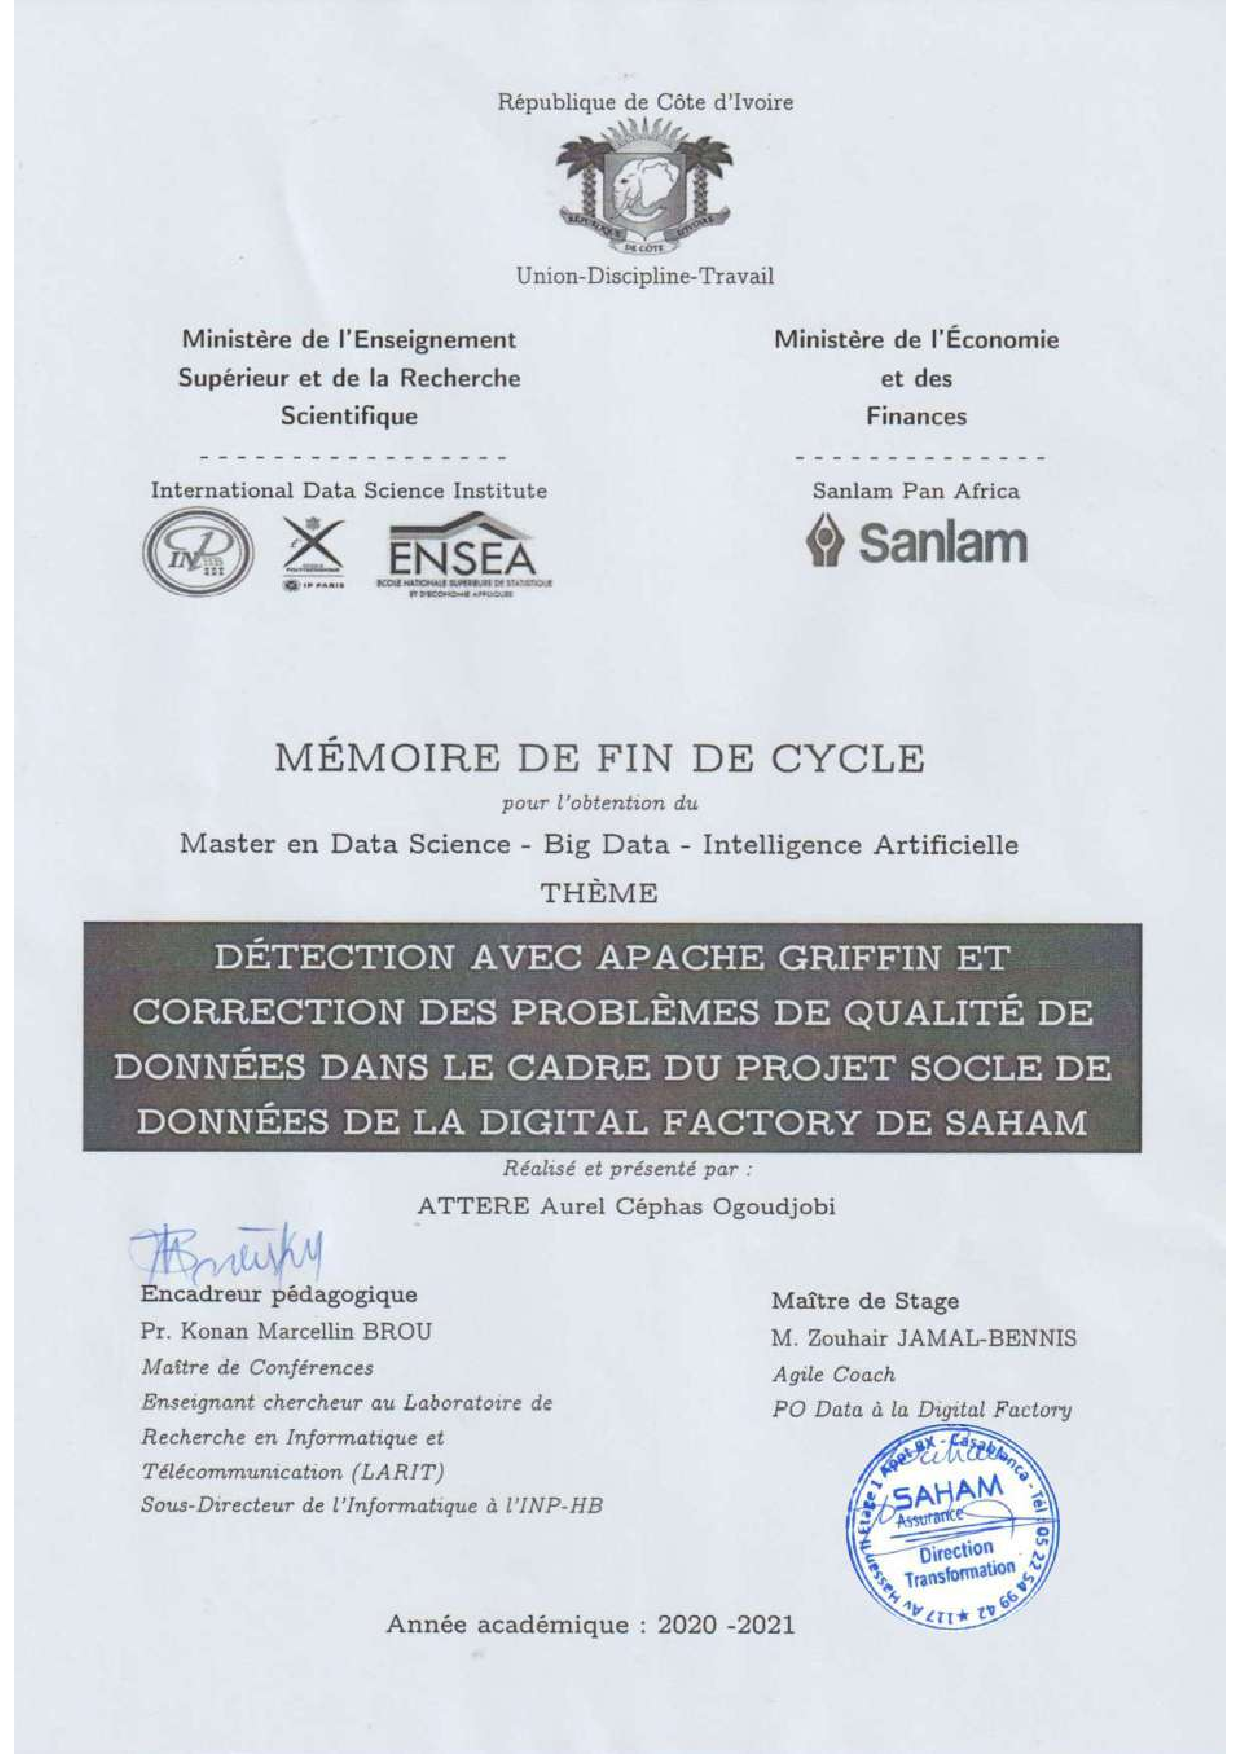
\includepdf{../Page_de_garde/Aurel_fr_signature_page-0001-1-ConvertImage}
%\tableofcontents
\addto\captionsfrench{\def\tablename{{Tableau }}}
%\addto\captionsfrench{\def\listingname{{Script }}}

\selectlanguage{french}
%Dedicace
\cleardoublepage
\phantomsection
\addcontentsline{toc}{chapter}{D\'edicace}
\chapter*{D\'edicace}
Je dédie ce mémoire à mes parents en témoignage de leurs multiples efforts et sacrifices quotidiens,
de même qu’à mes proches pour leur affection. Puisse ce travail vous rendre fier.
%Remerciements
\cleardoublepage
\phantomsection
\addcontentsline{toc}{chapter}{Acknowledgments}
\chapter*{ACKNOWLEDGMENTS}

\begin{small}
At the beginning of this work and before any development, it seems appropriate to thank first of all, Sanlam Pan Africa Group, for the opportunity it gave us to do our end of study internship at the \acrfull{df}, the digital pole of its Moroccan subsidiary Saham Assurance. We were welcomed by a wonderful, available and enthusiastic team. We would like to thank the members of the "Data" team for their availability; in particular, Mr. \textbf{JAMAL-BENNIS Zouhair} Agile Coach and Mrs. \textbf{SADIKI Fatimaezzahra} Data Engineer for their supervision and monitoring. We do not forget all the staff of Colina Participations who received us in an environment full of sympathy and good humor, which contributed to facilitate our integration. A special thanks to Mrs. \textbf{KADIA Essan}, Mr. \textbf{KOUASSI Dhom} and all the HR team for their kindness and contribution to the realization of this work.  \\

We thank Orange Group, the X Polytechnic Foundation, the X Polytechnic School of Paris, the \acrfull{inp} of Yamoussoukro and the \acrfull{ensea} of Abidjan who have done everything possible for the success of this training and continue to work on it. We also express our deep gratitude to the administration of \acrshort{inp}, in particular to Mr. \textbf{KOFFI N'Guéssan}  the former director general of \acrlong{inp}, \textbf{Dr. TANOH Lambert}, Director of the \acrshort{idsi}, to the teaching and administrative staff including \textbf{Dr. KADJO Lambert}, the Academic Director of \acrshort{idsi} and \textbf{Miss SORO Chantal} the executive assistant of \acrshort{idsi}. Our most distinguished thanks also go to our pedagogical supervisor, Professor \textbf{BROU Konan Marcellin} for having followed our work with diligence and rigor. 
\\

Finally, we would like to thank our fellow students of the $3^{rd}$ class of \acrshort{idsi}, our parents, brothers and sisters who have supported us morally and financially throughout this training. We express our deep respect to all those who took their time to read and correct this thesis.

\end{small}
%La rédaction de ce mémoire a été un travail de concert avec des personnes de bonne volonté qui nous ont soutenu et accompagné. ter

%\doublespacing
%\addtocontents{toc}{\itshape}
\renewcommand{\contentsname}{Table des matières}
%\cleardoublepage
\phantomsection
\addcontentsline{toc}{chapter}{Sommaire}
\shorttoc{SOMMAIRE}{1}
%\singlespacing

%Liste des tableaux
\cleardoublepage
\phantomsection
\addcontentsline{toc}{chapter}{\listtablename}
\listoftables

%Liste des illustrations
\cleardoublepage
\phantomsection
\addcontentsline{toc}{chapter}{Liste des figures}
\renewcommand{\listfigurename}{Liste des figures}
\listoffigures

%Sigles et abreviations
%\clearpage
\printnoidxglossary[type=acronym, title=Sigles et abr\'eviations, toctitle=Sigles et abr\'eviations]
\printglossary[type=\acronymtype]

\printglossary
%Avant-Propos
\cleardoublepage
\phantomsection
\addcontentsline{toc}{chapter}{Avant-Propos}
\chapter*{AVANT-PROPOS}

\begin{small}

%L'International Data Science Institute est une chaire internationale de formation en Data 
L'\acrlong{idsi} est une chaire internationale de formation en Data Science, Big Data et Intelligence Artificielle. Elle est issue d’un partenariat entre l'opérateur de  téléphonie Orange, l'\acrfull{inp}, l'\acrfull{ensea}, l'\'ecole X  Polytechnique et la Fondation de l'X Polytechnique. Homologuée par l'État de Côte d'Ivoire, la chaire a ouvert ses portes à la toute première promotion en 2017. Elle a pour objectif de former des experts dans le domaine de la Data Science, de l'Intelligence Artificielle et du Big Data.\\

D’une durée de deux ans, l’\acrshort{idsi} propose un master d’excellence de niveau international à destination d’étudiants qui s'approprient des connaissances en ingénierie informatique basée sur les nouvelles évolutions en matière de stockage et de traitement des données.  Pour parfaire la formation et se rapprocher du monde professionnel, il est prévu un stage de fin d'études sanctionné par la rédaction d'un mémoire puis une soutenance devant un jury constitu\'e d'enseignants de l'\acrshort{inp}, de l'\acrshort{ensea}, de l'X et de responsables d'entreprises. \\

C'est dans ce cadre, que nous avons effectu\'e \`a distance, un stage de 6 mois à la \acrlong{df} de Saham Assurance Maroc, qui est une filiale du Groupe Sanlam Pan Africa, tout en \'etant pr\'esent \`a Colina Participations.  Notre stage s'est d\'eroul\'e du 4 Mai 2021 au 27 Octobre 2021. Durant ce stage, nous avons travaill\'e sur \textit{« la d\'etection et la correction des problèmes de qualité de données dans le cadre du projet 'socle de données' de la \acrlong{df} »}, sous l’encadrement de Madame SADIKI Fatimaezzahra et Monsieur JAMAL-BENNIS Zouhair. Dans ce contexte, nous nous sommes efforcés de rester aussi fidèles que possible aux objectifs que la structure souhaite atteindre en r\'ealisant ce travail de recherche.

\end{small}

%\chapter*{SIGLES ET ABREVIATIONS }



%Resume - Abstract
\newpage
\cleardoublepage
\phantomsection
\addcontentsline{toc}{chapter}{R\'esum\'e}
\section*{R\'ESUM\'E}

\`A l'\`ere du \textit{big data}, la qualité de toute décision dépend de la qualité des données utilisées. En effet, en l’absence de données fiables, une entreprise peut prendre potentiellement de mauvaises décisions. Notre \'etude vise dans un premier temps, \`a d\'etecter avec Apache Griffin les probl\`emes de qualit\'e sur les donn\'ees du projet socle de donn\'ees de la Digital Factory de Saham Maroc, puis \`a appliquer des correctifs lorsque cela est possible. De l'analyse th\'eorique effectu\'ee, nous avons retenu que la qualité des données, désigne l’aptitude de l’ensemble des caractéristiques intrinsèques des données (compl\'etude, cohérence, unicité, validit\'e, exactitude,actualit\'e) à satisfaire des exigences internes et des exigences externes à l’organisation. Pour pouvoir l'\'evaluer efficacement, nous avons eu recours \`a Apache Griffin. Il s'agit d'une plateforme \textit{big data}, qui offre des services de qualit\'e de donn\'ees. Elle permet d'\'editer des r\`egles de qualit\'e et de stocker les m\'etriques \`a des fins de visualisation ou d'historisation. L'\'evaluation de la qualit\'e des  extractions tables des 'Detail\_Victimes' et 'Inventaire\_Sinistre', a permis de relever plusieurs incoh\'erences que nous avons corrigées en utilisant PySpark, au moyen d'algorithmes de redressement.\\
\textbf{Mots cl\'es}: qualit\'e, donn\'ees, \textit{big data}, \'evaluation, correction, Griffin, anomalies
\section*{ABSTRACT}

In the age of big data, the quality of any decision depends on the quality of the data used. Indeed, without reliable data, a company can potentially make bad decisions. Our study aims, first, to detect with Apache Griffin the quality problems on the data of the Digital Factory of Saham Maroc, then to apply corrective measures when possible. From the theoretical analysis carried out, we have retained that data quality refers to the ability of all the intrinsic characteristics of the data (completeness, consistency, uniqueness, validity, accuracy, timeliness) to meet internal requirements and external requirements to the organization. To be able to evaluate it efficiently, we used Apache Griffin. It is a big data platform, which offers data quality services. It allows editing quality rules and store metrics for visualization or historical purposes. The quality assessment of the 'Detail\_Victime' and 'Inventaire\_Sinistre' extraction tables revealed several inconsistencies that we corrected using PySpark, by means of a rectification algorithm.\\
\textbf{Key words}: quality, data, big data, evaluation, correction, Griffin, inconsistencies

%Introduction Generale
\cleardoublepage
\phantomsection
\addcontentsline{toc}{part}{INTRODUCTION G\'EN\'ERALE}
\pagenumbering{arabic}
\vspace*{0.5cm}
\section*{\centering \Huge Introduction G\'en\'erale}
\titlerule[2.0pt]
\vspace{1cm}
 %Pour les entreprises, c'est un moyen d'augmenter significativement leur profit sur une période donnée. Ainsi, \`a travers les innovations techniques qu'elles induisent, les diff\'erentes r\'evolutions industrielles ont profondément  transformé l'économie. [...] Bien que déjà visible dans ses réalisations comme l’intelligence artificielle, la nanotechnologie ou l’information quantique, nous en sommes qu’au début.%
%En \'economie, le progrès technique est considéré comme une source majeure de croissance surtout pour les entreprises. Ainsi, 
Le monde fait face aujourd'hui aux prémices d’une quatrième révolution industrielle favoris\'ee par l'essor du \textit{big data}. \`A travers les innovations techniques qu'elles induisent, les diff\'erentes r\'evolutions industrielles ont profondément transformé l'économie et significativement augment\'e le profit des entreprises. Ainsi, l'explosion du volume des donn\'ees de m\^eme que l'apparition et la vulgarisation de nouvelles technologies de stockage, de traitement et de mise en valeur des donn\'ees, ont suscité de profonds changements au sein des entreprises. Afin de profiter des externalit\'es de cette r\'evolution, les entreprises sont de plus en plus tourn\'ees vers des approches \textit{data-driven} et \textit{data-centric}. Cela se manifeste \`a travers une architecture dans laquelle les données constituent l'actif principal.  Aujourd'hui, les entreprises effectuent des analyses \textit{big data}, des modélisations de diagnostic et des traitements de données pour atteindre l'excellence sur le marché. Il va donc sans dire que toute entreprise souhaitant s'inscrire dans une dynamique \textit{data-driven} et \textit{data-centric} se doit d'avoir des donn\'ees de qualit\'e sur lesquelles s'appuyer. Dans le cas contraire, vous imaginez bien les décisions désastreuses qu'elle  pourrait prendre. Il est alors n\'ecessaire, voire primordial pour toute entreprise de se doter d'une solide strat\'egie de gouvernance des donn\'ees et donc de qualit\'e des donn\'ees.\\

Fort de ce constat, Saham Assurance Maroc \`a travers sa \acrlong{df}, a d\'ecid\'e de mettre en place dans le cadre de son projet socle de donn\'ees, une politique de gouvernance des donn\'ees. Cette derni\`ere, donne une attention particuli\`ere au volet qualit\'e. En effet, la qualit\'e des donn\'ees revêt un aspect très important pour les entreprises d'assurances, en ce sens qu'elle facilite grandement l'activit\'e de l'assureur dans la d\'etermination des risques, le calcul des tarifications et même la d\'etection des fraudes, sans oublier les exigences réglementaires du r\'egime prudentiel Solvabilit\'e 2. C’est dans ce contexte que le sujet suivant : \textit{« détection et correction des problèmes de qualité de données dans le cadre du projet socle de données »}, nous a été confié durant nos six mois de stage \`a la Digital Factory de Saham Assurance Maroc.\\

L'objectif principal de cette \'etude est de d\'etecter avec Apache Griffin les probl\`emes de qualit\'e de quelques tables du socle de donn\'ees, puis d'appliquer lorsque cela est possible des algorithmes de correction des anomalies d\'etect\'ees. Pour cela, nous avons suivi une m\'ethodologie en trois (3) grandes \'etapes : 
\begin{itemize}[parsep=0cm,itemsep=0cm]
    \item l'installation et la configuration d'Apache Griffin afin de r\'epondre aux exigences en terme de plateforme de qualit\'e de donn\'ees;
    \item l'utilisation d'Apache Griffin pour la d\'etection des anomalies et incoh\'erences dans les donn\'ees du socle et;
    \item la proposition d'algorithmes de correction.
\end{itemize}
Avant d'aborder et d'appliquer cette m\'ethodologie, nous allons dans un premier chapitre situer l'\'etude dans son cadre contextuel en pr\'esentant l'entreprise ainsi que les d\'etails du projet. Le deuxi\`eme chapitre  quant \`a lui permettra de mieux comprendre les réflexions théoriques sous-jacentes. Ces deux premiers chapitres constituent la premi\`ere partie du pr\'esent m\'emoire. Dans une seconde partie, nous procéderons à la description détaillée en deux chapitres \'egalement, des r\'esultats obtenus en appliquant la m\'ethodologie ci-dessus \'enonc\'ee. 




%\Partie 1 
\part{\normalfont \LARGE CADRE INSTITUTIONNEL ET TH\'EORIQUE DE L'\'ETUDE}
%Chapitre1
\chapter{Cadre institutionnel de l'\'etude }
\section*{Introduction}
Le cursus en Master 2, est sanctionn\'e par la r\'edaction et la soutenance d'un m\'emoire de fin de formation. Afin de valider notre dipl\^ome, il est n\'ecessaire d'effectuer un stage, au cours duquel nos acquis th\'eoriques seront r\'einvestis pour solutionner des probl\`emes m\'etiers. Ce chapitre pr\'esente le cadre institutionnel de notre stage et le sujet qui nous a \'et\'e confi\'e. Apr\`es une pr\'esentation de la structure d'accueil et de la probl\'ematique, nous allons exposer le cahier de charges ainsi que la m\'ethode de travail adopt\'ee.

\section{Cadre contextuel}

\subsection{Pr\'esentation de l'organisme d'accueil}
\subsubsection{\textbf{Sanlam Group}}
Fondée en 1918 en tant que compagnie d’assurance vie, Sanlam (South African National Life Assurance Company Limited) est aujourd’hui un groupe leader des services financiers diversifiés, basé en Afrique du Sud. Il déploie ses activités à travers l’ensemble du continent africain ainsi qu’en Malaisie, aux Etats-Unis, en France, en Suisse, en Inde et en Australie. Groupe financier de référence coté à la bourse de Johannesburg, Sanlam offre des solutions financières complètes et personnalisées dans tous les segments du marché, à travers ses cinq (5) pôles d’activités : Sanlam Personal Finance, Sanlam Pan-Africa, Sanlam Investments, Sanlam Corporate et Santam (South African National Trust and Assurance Company Limited).
\begin{figure}[!h]
  \caption{Organigramme de Sanlam Group}  \label{fig:xray}
  \begin{center}
  \hspace*{-1.0in}
  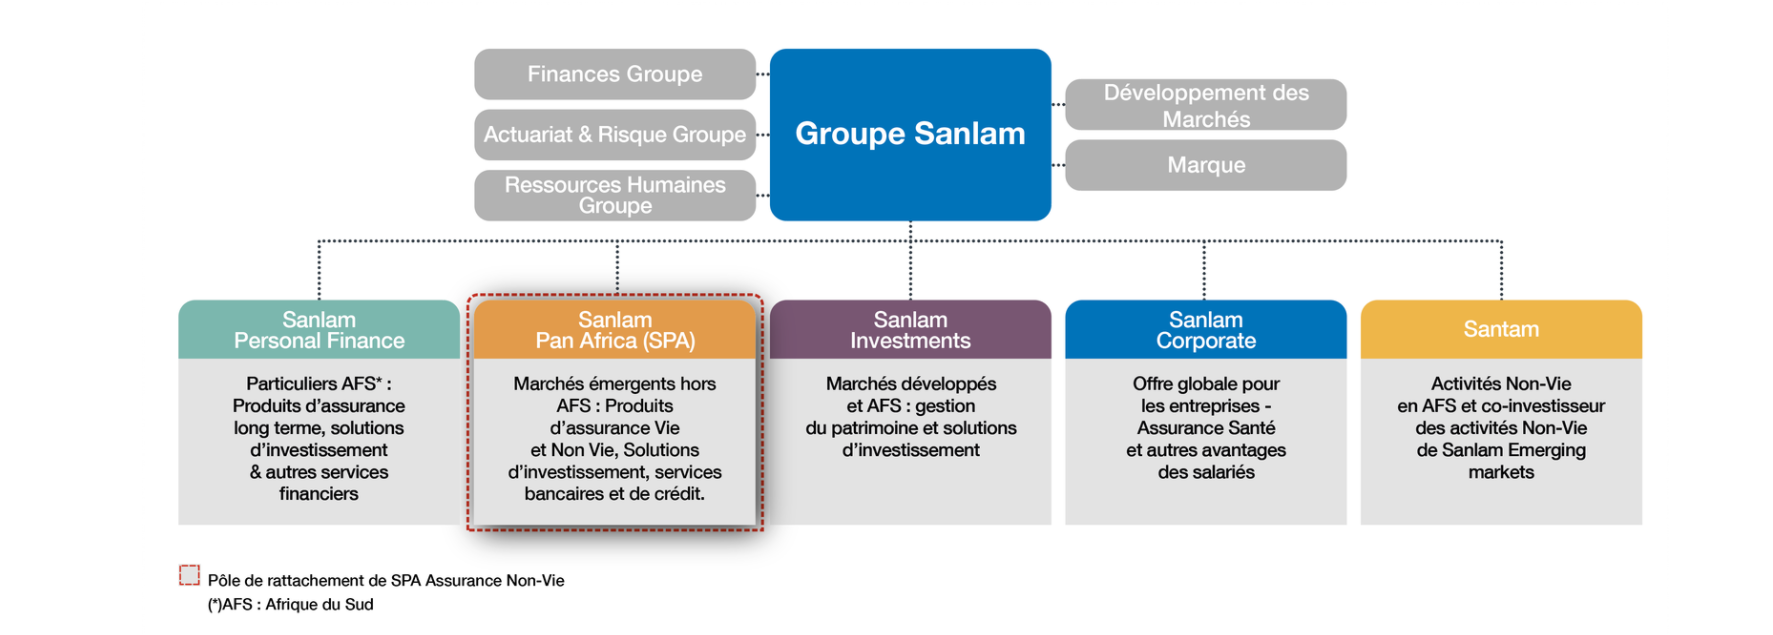
\includegraphics[scale=0.30]{Static/Organigramme.png} 
  \end{center}
\end{figure}
\\

C'est l'un des plus grands groupes d'assurance ayant une couverture internationale, dans le monde, en termes de présence, avec une présence directe et indirecte dans quarante-quatre (44) pays, à l'exception de l'Afrique du Sud. Sanlam Group, fournit plus précisément des solutions et produits financiers aux particuliers et aux entreprises \`a savoir :
\begin{itemize}[parsep=0cm,itemsep=0cm]
\item la planification financière et conseil;
\item l'assurance vie et non vie, la r\'eassurance;
\item la gestion de patrimoine, interm\'ediaire boursier;
\item la gestion des fonds (pensions, retraites,...).
\end{itemize}
%\vspace {0.5cm}
%\paragraph{}

\`A  Sanlam Group, on développe une vision portée sur la création de valeur pour le client, placé au cœur de toute stratégie de développement. Par ailleurs, il ambitionne de consolider ses positions sur le segment des solutions d’investissement sur les marchés développés. 
%Sa vision strat\'egique est de créer de la valeur durable pour toutes les parties prenantes. Elle se d\'ecline sur 3 axes principaux:
%\begin{itemize}[parsep=0cm,itemsep=0cm]
%\item pour l'Afrique du Sud : \^etre leader dans la gestion de patrimoine, le management et la protection;
%\item pour l'Afrique, l'Inde, la Malaisie et le Liban : \^etre un Groupe de services financiers panafricain de premier plan avec une présence significative en Inde et en Malaisie;
%\item pour les march\'es d\'evelopp\'es : se positionner sur la niche de gestion du patrimoine et de placements sur des marchés développés spécifiques.
%\end{itemize}
%\vspace {0.5cm}
Au sein du Groupe, notre stage s'est d\'eroul\'e au p\^ole Sanlam Pan-Africa. 
\subsubsection{\textbf{Sanlam Pan-Africa}}
\acrfull{spa} est le pôle d’activités de Sanlam Group opérant sur les marchés émergents (hors Afrique du Sud). \acrshort{spa} assure ainsi le développement et le déploiement d’une gamme diversifiée de produits d’assurance Vie et Non-Vie, ainsi que des solutions d’investissement, des services bancaires et de crédit à la consommation, la bancassurance, la gestion d’actifs et des produits d’assurances Non-Vie spécialisées pour l’Afrique, l’Inde, la Malaisie et le Liban. L’Afrique est aujourd’hui une composante fondamentale de la vision de Sanlam Group, d’où la mission stratégique fondamentale dévolue à \acrshort{spa} : ériger un groupe de services financiers panafricain de premier plan. Disposant de la première empreinte panafricaine qui lui garantit un rayonnement continental unique, \acrshort{spa} se positionne notamment en tant que partenaire privilégié des multinationales et autres réseaux de distribution. Au sein de SPA, nous avons effectu\'e notre stage \`a la \acrfull{df} de Saham Maroc, afin de b\'en\'eficier d'un suivi ad\'equat.

\subsubsection{\textbf{Digital Factory }} 
La \acrlong{df}, est un espace où des experts en digital travaillent et r\'efl\'echissent sur l’accélération de la transformation digitale et l’élaboration de solutions pour une expérience client optimale. La \acrshort{df} se veut \textit{customer centric} et proactive pour livrer des produits efficaces et utiles
pour les métiers en un temps record. Pour cela, en plus des compétences recrutées et de leurs expériences, elle mise sur une approche organisationnelle du travail : l’agilité à travers la méthode Scrum\footnote{concept d\'efini \`a les section 1.2.3}. Grâce à la \acrlong{df}, Saham Assurance Maroc innove sur des produits qu’elle lance au fur et à mesure. Elle comprend plusieurs \'equipes constituées aussi bien de d\'eveloppeurs, d'\acrfull{ui_ux} designers, de \textit{data scientists}, \textit{data engineers}, \textit{data architects}, de coach agile...
\\

En raison des conditions sanitaires, notre stage s'est effectu\'e physiquement \`a Colina Participations (qui est la \textit{holding} du groupe Sanlam d\'etenant les parts dans les diff\'erentes filiales en Afrique hors Maroc et Afrique du Sud) mais virtuellement (\`a distance) \`a la \acrlong{df}. Nous avons \'et\'e suivis et encadr\'es dans un environnement convivial et agile. Ce stage nous a permis d'\^etre beaucoup plus autonome et de pouvoir transformer les besoins m\'etiers ainsi que les contraintes \textit{business} en r\'ealisations techniques.  


\subsection{Qualit\'e des donn\'ees en assurance}
L'assurance est un secteur qui a pour principale mission de fournir une prestation lors de la survenance d'un événement incertain et aléatoire souvent appelé 'risque'. La prestation, généralement financière, peut être destinée à un individu, une association ou une entreprise, en échange de la perception d'une cotisation ou prime. L'assurance se d\'efinit aussi comme \'etant une op\'eration par laquelle l'assur\'e transf\`ere ses risques \`a l'assureur en contrepartie du paiement d'une prime. 
\\

Bien qu'\'etant un secteur majeur dans les activit\'es \'economiques d'un pays, l'assurance se distingue par l'inversion du cycle de production. En effet, il est impossible aux compagnies de savoir avec certitude, combien la prestation qu’elles vendent leur coûtera, la prime étant payée par le client avant l'indemnisation. Ainsi, pour fixer le montant de sa prime ou calculer les provisions, l’assureur ne peut se baser que sur des études statistiques lui permettant de se faire une idée de combien lui coûtera sa prestation en analysant par exemple le taux de sinistralité et le co\^ut moyen des sinistres ant\'erieurs. Cela ne donne pas pour autant la certitude qu’il n’aura pas à faire face à des sinistres majeurs (en termes de fr\'equence ou de co\^ut). La fiabilité des systèmes d’information et la qualité des données doivent alors constituer un objectif permanent, dans un environnement  incertain et malgr\'e tout concurrentiel.  \\
 

Ce sujet est donc au cœur du modèle d’affaires des assureurs. La parfaite maîtrise des systèmes d’information et des dispositifs de sécurité sont des leviers stratégiques voire vitaux pour maintenir une position de leader dans le domaine. Elle permet notamment de  : 

\begin{itemize}[parsep=0cm,itemsep=0cm]
\item se distinguer en termes de tarification, gr\^ace à une segmentation plus efficiente avec la possibilité de créer de nouvelles offres ;
\item se distinguer en termes de gestion des risques, par une optimisation des couvertures et des provisions;
\item mettre en place de meilleurs systèmes de détection des fraudes.
\end{itemize}    
L’enjeu est crucial à tous les niveaux : que ce soit pour une bonne appréhension des risques, pour mener les études actuarielles, réaliser les tarifications, évaluer les provisions ou fiabiliser les modèles, etc. \\

Les organismes assureurs sont donc, sensibles aux gains de productivité espérés qui pourront se traduire dans la compétition avec les autres acteurs du marché. De ce fait, les défauts de qualité des données peuvent constituer un frein à la compétitivité du groupe face aux concurrents et s’avérer être coûteux pour plusieurs raisons. Tout d’abord, ils (les d\'efauts de qualit\'e) rendent plus difficiles l’ensemble des travaux de production puisqu’ils complexifient les traitements. De plus, des données de mauvaise qualité sont susceptibles de conduire à une dégradation ou à l’allongement des travaux et des analyses qui en résultent. Enfin, elles impactent la qualit\'e des services offerts aux clients. En effet, selon une étude du \acrfull{mit} (MIT, 2017) \cite{MIT2017}, la non-qualité occasionne une perte d'argent estimée entre 15\% et 25\% du chiffre d’affaires total de la plupart des entreprises. Environ 20 ans plus t\^ot, cette perte s'\'evalue \`a 5\% - 10\% du revenu des entreprises \cite{Techno7}. De m\^eme, dans \cite{efrontech},  l’institut Gartner estime que plus de 25\% des données des plus grandes entreprises mondiales sont erronées et précise \'egalement qu'un tel probl\`eme n’a pas une conséquence informatique mais plut\^ot une cons\'equence commerciale, se chiffrant en millions de devises mon\'etaires. Cette perte représentant environ un quart des revenus, s’explique par les mauvais choix stratégiques opérés à partir d’informations erronées, mais aussi par le temps perdu par les services informatiques à traiter ces données inexactes:  contr\^oles, corrections et maintenances. Ramener au secteur de l'assurance, une non-qualit\'e des donn\'ees peut nuire aux décisions prises s’agissant aussi bien des exigences r\'eglementaires que des choix strat\'egiques de l’entreprise (mauvaise interprétation de la situation actuelle par exemple) \cite{Axysweb_Consequences}. Prendre une décision à partir de mauvaises informations affecte l’entreprise, ses clients ou ses partenaires.
\\

La d\'efinition d'une bonne strat\'egie de gouvernance des données est un sujet qui prend de l’importance dans les entreprises et les administrations. Il urge alors de se pencher plus s\'erieusement sur cette probl\'ematique tout en prenant en compte le contexte technologique. Il est impensable que les données de l’assureur ne soient pas à la hauteur des attentes. Une défaillance sur ce volet-là a de lourdes conséquences. Point d'ancrage de toute strat\'egie de gouvernance des donn\'ees, la mise en place d'un projet de qualit\'e des donn\'ees requiert quelques interrogations: qu'est-ce que la qualit\'e des donn\'ees et comment la mesurer? Quels sont les diff\'erents outils de qualit\'e des donn\'ees et quels sont les avantages qu'offre Apache Griffin vis-\`a-vis de ces derniers? Comment corriger les probl\`emes de qualit\'e des donn\'ees d\'etect\'es?


%%\section{M\'ethodologie de recherche}

%Lorem ipsum dolor sit amet, consectetur adipiscing elit. In maximus imperdiet mauris, eu tempor diam pulvinar ut. Etiam dignissim ultrices eros, pellentesque feugiat libero pharetra sit amet. Praesent et lacinia augue. Sed eget mi sit amet elit fringilla commodo. Maecenas finibus est velit, vitae commodo ante dictum at. Fusce nec nibh non mauris sollicitudin tempor vel sed ligula. Donec ac dictum risus. Maecenas consectetur turpis eget egestas faucibus. Vestibulum pretium suscipit diam, vitae feugiat ex tempus ut. Proin elementum faucibus est non porta. Aliquam sed sapien est. 
%\subsection{Objectifs }
%\subsection{Questions de recherche}
%\subsection{M\'ethode de recherche}
%\subsection{Valeur du travail}

%\section{\'Etude de l'existant}
%\`A la Digital Factory de Saham Maroc, suite \`a l'absence de moyen de v\'erification de la qualit\'e des donn\'ees, aux incoh\'erences rencontr\'ees dans le calcul des primes et aux difficult\'es dans la r\'ealisation de regroupement fiable, le besoin s'est fait ressentir de mettre en place un outil permettant d'industrialiser la gestion de la qualit\'e des donn\'ees . Cet outil viendra remplacer les tests manuels (SQL) et les explorations effectu\'ees sans industrialisation. 
%\section{Management du projet}

%(Une introduction partielle)

\section{Terms of reference}
The \acrlong{df} has developed a data base in agile mode to modernize and digitalize certain business processes. In order to achieve these objectives and develop new Business Intelligence capabilities at the Group level, it is necessary to :
\begin{itemize}[parsep=0cm,itemsep=0cm]
    \item review the functional and technical architecture in order to make the data base more robust and scalable but also;
    \item implement a data governance program to improve data quality.
\end{itemize}
\subsubsection{\textbf{Overall objective }}
%L'objectif g\'en\'eral est de d\'etecter et de corriger les probl\`emes de qualit\'e de donn\'ees dans le cadre du projet socle de donn\'ees de la Digital Factory. La d\'etection se fera \'a l'aide de l'outil Apache Griffin. Il est de ce fait subdiviser en deux volets : le volet outil et le volet correctif.

The general objective of our subject is to evaluate in a first step with the help of Apache Griffin, the quality of the \acrlong{df}'s data. And then to proceed to a correction of the various detected anomalies. It is thus subdivided into two parts:
a tool component and a detection and correction component.
\subparagraph{\textbf{> Tool component: Specific objectives}} The purpose of this component is to :
\begin{enumerate}[parsep=0cm,itemsep=0cm]
    \item take in hand the data quality audit tool Apache Griffin ;
    \item establish the connection with the different databases;
    \item analyze the perspectives offered by this tool.
\end{enumerate}
\subparagraph{\textbf{> Detection and correction component: Specific objectives}} The aim here is to use the tool to identify the various data quality problems and, if necessary, propose corrective measures. More specifically, it will be necessary to do:
\begin{enumerate}[parsep=0cm,itemsep=0cm]
    \item a review of the different data in the base and detect inconsistencies with the different data and extractions used by the business;
    \item a prioritization of the main fields to be improved;
    \item an implementation of data rectification algorithms when possible ;
    \item possibly an injection of open data to improve the quality of prioritized data.
\end{enumerate}

\section{Analysis of the existing situation}
Data quality auditing at the \acrlong{df} is not a new issue. It was done by means of manual exploration of the data and \acrshort{sql} (\acrlong{sql}) queries. This method did not allow for a real industrialisation of the quality assessment and was carried out after the fact. Indeed, it did not offer the possibility of monitoring the evolution of metrics over time, which is very important in the quality management process. Moreover, the absence of a real upstream verification tool for data quality prevents the preventive detection of irregularities. These inconsistencies are only detected at the data enhancement stage, requiring exploration of the data to identify the sources of irregularity. All this has an impact on the productivity and performance of the company. The idea of working on the exploration of a data quality audit tool is at several levels. Firstly, a tool dedicated to data quality would allow it to be easily integrated into the production chain. Secondly, the choice of the tool should correspond to the requirements of the \acrshort{df} in terms of detection and malleability.
%\subsection{M\'ethode de travail agile}
%La méthode Agile est une méthodologie de gestion de projet. Il s'agit d'une organisation de travail en cycles courts, permettant aux équipes de développement de gérer un produit de manière souple, adaptative et itérative. Pour cela, elle place le client au cœur du projet et s’adapte tout le long  du projet. De plus, au lieu de planifier le projet de A à Z dès le départ, ce qui laisse peu de place aux imprévus, des objectifs courts sont fixés, par exemple à deux ou trois semaines. Le projet est divisé en sous-projets et l’on ne passe au suivant que lorsque le précédent est réglé. Le principal avantage est la flexibilité, la possibilité de s’adapter en fonction des nouvelles exigences du client ou des évolutions du marché. \\
%Il existe en réalité plusieurs méthodes qui ont toutes un point commun : elles découlent toutes du Manifeste Agile. Scrum est aujourd’hui l’approche Agile la plus répandue; il s'agit plus précisément d'un cadre m\'ethodologique plut\^ot que d'une m\'ethode. Elle est d'ailleurs celle impl\'ement\'ee par la \acrshort{df}. De plus, Scrum est une pratique Agile élémentaire qui permet également une mise à l’échelle, autrement dit le déploiement progressif de l’agilité à l’échelle de l’entreprise. 
%Scrum est constitué d'une définition des rôles, de réunions et d'artefacts \cite{Nutcache_agile} \cite{Agiliste_agile}. 
%\subsection{Organisation et planning du projet (d\'ecrire l'impl\'ementation du scrum dans le cadre du projet et les sprints --Not Yet Done)}


\section*{Conclusion}
La \acrlong{df} de Saham Maroc, est un espace où des experts en digital travaillent et réfléchissent sur l’accélération de la transformation digitale et l’élaboration de solutions innovantes dans une approche \textit{data-centric}. Elle a mis en place un programme de gouvernance de donn\'ees afin d'am\'eliorer la qualit\'e des donn\'ees de son socle de donn\'ees. Notre projet porte sur le volet qualit\'e o\`u il s'agira de d\'etecter et de corriger les probl\`emes de qualit\'e. Des donn\'ees de bonne qualit\'e permettront \`a Saham Assurance Maroc de pouvoir se distinguer notamment en termes de tarification et en termes de gestion des risques. Le chapitre suivant fera l'objet d'une pr\'esentation du cadre th\'eorique et m\'ethodologique de notre \'etude.
%Chapitre2
\chapter{Cadre th\'eorique et m\'ethodologique de l'\'etude}
\section*{Introduction}
Les difficult\'es en mati\`ere de qualité des données ne sont pas exclusivement liées aux technologies de l'information, mais il s’agit plutôt d’une problématique qui concerne en grande partie les processus de l’entreprise. Pour mener à bien la présente étude, il est nécessaire d’effectuer un point th\'eorique afin de mieux la situer dans le contexte et de comprendre les r\'eflexions sous-jacentes. Ainsi, ce chapitre fait un résumé de l’existant en matière de cadre d'analyse de la qualit\'e des donn\'ees et amorce la compr\'ehension de l'outil de qualit\'e Apache Griffin. Suite \`a une clarification conceptuelle, nous ferons la lumi\`ere sur les dimensions de qualit\'e de donn\'ees tout en abordant la question des mesures correctives et celle de l'outil \`a choisir.
\section{Clarification conceptuelle}

\subsection{Big Data}
%Pour pouvoir, les utiliser au mieux dans son organisation et son processus décisionnel, il est essentiel de maîtriser les principes et caractéristiques clés du \textit{big data}.
%Le \textit{big data} (donn\'ees massives), fait désormais partie du quotidien de toutes les entreprises. 
Le terme \textit{big data} a été popularisé par John Mashey, informaticien chez Silicon Graphics dans les années 1990 \cite{Cairn_5V}. Ce dernier faisait r\'ef\'erence aux bases de données trop grandes et complexes pour être étudiées avec les méthodes statistiques traditionnelles – et, par extension, à tous les nouveaux outils d’analyse de ces données. En 2001, Douglas Laney a analysé cette nouvelle tendance à travers une liste très simple de trois \textit{« V »}, ensuite élargie à cinq \textit{« V »} \cite{Cairn_5V} \cite{Talend_5V} :
\begin{itemize}[parsep=0cm,itemsep=0cm]
\item le volume : pour d\'esigner la grande quantit\'e de donn\'ees ou d'informations contenues dans ces bases de donn\'ees;
\item la v\'elocit\'e : \'egalement appel\'ee vitesse, correspond à la rapidité à laquelle les donn\'ees sont générées, collect\'ees et circulent pour transmission et analyse;
\item la vari\'et\'e : pour désigner la multiplicité des types de données disponibles, autrement dit les différences de natures, formats et structures \footnote{Donn\'ees structur\'ees, semi-structur\'ees ou non structur\'ees\\};
\item la valeur :  fait r\'ef\'erence \`a la capacit\'e de ces donn\'ees \`a g\'en\'erer du profit; chaque donnée devant apporter une valeur ajoutée à l’entreprise; 
\item la v\'eracit\'e : qui permet de garantir la qualité et la fiabilité des données.
\end{itemize}

%Ces cinq \textit{« V »} permettent donc de d\'ecrire et de caract\'eriser les \textit{big data}. 
Nous nous intéressons ici à cette dernière caract\'eristique. En effet, pour pouvoir tirer de la valeur des donn\'ees, la qualit\'e est la condition pr\'ealable à l'analyse et à l'utilisation du \textit{big data}. D’où la nécessité de prendre des mesures de précaution pour minimiser les biais liés au manque de fiabilité des données. Les méthodes permettant d'améliorer et de garantir la qualité des \textit{big data} sont essentielles pour prendre des décisions commerciales précises, efficaces et fiables. Mais qu'est-ce qu'une donn\'ee de qualit\'e?

%ainsi qu'\`a la garantie de leur valeur

%Dans un contexte o\`u, le volume de données augmente de manière exponentielle, ce sont généralement les entreprises qui commencent à tirer des avantages incroyables de leurs \textit{big data}. Selon les gestionnaires et les économistes, les entreprises qui ne s’intéressent pas sérieusement au \textit{big data} risquent d’être pénalisées et écartées \cite{Lebigdata_5V}. 

%de la valeur contenue dans ces donn\'ees, il leur faut avoir des donn\'ees de qualit\'es, fiables, cr\'edibles et pr\'ecises faisant ainsi r\'eference \`a la v\'eracit\'e.

\subsection{Qualit\'e des donn\'ees}
Définir la qualité des données n’est pas une op\'eration ais\'ee. On est bien souvent tent\'e de définir plut\^ot la non-qualité \cite{pwc_micro_ebg_2011}. Afin de mieux saisir cette notion, nous d\'efinirons d'abord ce qu'on entend par qualit\'e, information et donn\'ee avant de revenir sur la d\'efinition de la qualit\'e des donn\'ees en elle-m\^eme. \`A cet effet, d'apr\`es l'organisation internationale de normalisation (\acrfull{iso}) \cite{Iso8000}, la  qualit\'e pourrait se d\'efinir comme le degré auquel un ensemble de caractéristiques inhérentes à un objet répond aux exigences. On parle \'egalement de conformit\'e aux exigences. Toujours selon l'\acrshort{iso} \cite{Iso8000}, l'exigence se d\'efinit comme un besoin ou une attente énoncée; généralement implicite ou obligatoire. 
Dans \cite{pwc_micro_ebg_2011}, on retiendra que les donn\'ees \emph{« sont des faits et des statistiques qui peuvent être quantifiées, mesurées, comptées, et stockées »} et que l'information quant \`a elle \emph{« est un ensemble de données organisées selon une ontologie\footnote{Une ontologie est l'ensemble structuré des termes et concepts représentant le sens d’un champ d'informations (wikipedia)} qui définit les relations entre certains sujets»}.\\

La qualit\'e des donn\'ees pourrait donc se d\'efinir plus précisément, comme le degré auquel un ensemble de caractéristiques inhérentes aux données répond aux attentes énoncées \cite{Iso8000}. Mais plus loin, Wang et Strong(1996) cit\'es par Cai et Zhu \cite{Cai_Zhu_2015},  d\'efinissent la qualit\'e comme l'aptitude \`a l'emploi et proposent que le jugement de la qualité des données dépende des consommateurs de données. L'objectif est d'avoir \`a disposition des donn\'ees exemptes d'erreurs, d'incohérences, de redondances, de formatage médiocre et d'autres problèmes susceptibles d'empêcher une utilisation aisée \cite{PreciselyDQ}. Ces deux d\'efinitions font ressortir deux aspects tr\`es importants qui se reflètent \'egalement dans la litt\'erature. En effet, tous les auteurs s'accordent sur le fait que la qualit\'e dépend non seulement des caractéristiques propres aux donn\'ees, mais aussi de l'environnement dans lequel ces donn\'ees sont utilis\'ees.
\\

Cette perception met ainsi en exergue le caract\`ere subjectif de cette notion. Aussi peut-on lire \cite{WikiDQ}, que : 
\begin{itemize}[parsep=0cm,itemsep=0cm]
\item pour le consommateur par exemple, des donn\'ees de qualit\'e sont des données : 
\begin{itemize}[parsep=0cm,itemsep=0cm]
\item qui sont aptes à être utilisées ;
\item qui répondent \`a ses attentes ou les dépassent et;
\item  qui satisfont aux exigences de leur utilisation prévue;
\end{itemize}
\item il en est de m\^eme, pour l'entreprise qui de façon sp\'ecifique, inscrit cette d\'efinition dans un cadre op\'erationnel, d\'ecisionnel et commercial;
%\begin{itemize}
%\item  qui sont aptes à être utilisées dans leurs rôles opérationnels, décisionnels et autres prévus ou qui présentent une conformité aux normes qui ont été fixées;
%\item  qui sont adaptées aux utilisations prévues dans le cadre des opérations, de la prise de décision et de la planification et ;
%\item  capable de satisfaire les exigences commerciales, systémiques et techniques déclarées de l'entreprise;
%\end{itemize}
\item par contre, du point de vue des normes, la qualit\'e des donn\'ees est mesur\'ee par :
\begin{itemize}[parsep=0cm,itemsep=0cm]
\item le degré auquel un ensemble de caractéristiques (dimensions de qualité) répond aux exigences ainsi que;
\item l'utilité, la précision et l'exactitude des données pour leur utilisation.
\end{itemize}
\end{itemize}

Cette diversit\'e de point de vue, se justifie par le fait qu'avec l'av\`enement du \textit{big data} contrairement au pass\'e, les utilisateurs de données ne sont pas nécessairement les producteurs de ces données; renforçant de ce fait l'absence d'une d\'efinition unique. Abondant dans le m\^eme sens, sur la d\'efinition de la qualit\'e des donn\'ees, le \acrfull{niss} \cite{NISS_2001} identifie sept(7) principes cl\'es permettant de saisir sa quintessence. Ainsi, ils \'enoncent que les donn\'ees peuvent \^etre vues comme un produit et leur qualit\'e  d\'epend de multiples facteurs et qu'en principe, la qualit\'e peut \^etre  mesurée et améliorée.
\\

Plusieurs dimensions entrent en jeu dans la définition de la qualité. Chacune, décrivant des caractéristiques qui peuvent être mesurées ou évaluées par rapport à des attentes spécifiques \cite{dama}. Le caract\`ere mesurable des dimensions s'av\`ere nécessaire pour leur quantification dans la pratique. On parle alors de m\'etrique. Une métrique de qualit\'e des donn\'ees selon Ehrlinger, Rusz et Wöß \cite{ehrlinger2019survey}, est une fonction qui \`a une dimension de qualité associe une valeur numérique. Une telle métrique peut être calcul\'ee à différents niveaux d'agrégation : au niveau des valeurs, des colonnes ou des attributs, des tuples ou des enregistrements, des tables ou des relations, ainsi qu'au niveau de la base de données. S'adaptent-elles bien au \textit{big data}?
\\

\`A la faveur de cette clarification conceptuelle, on pourrait alors se demander comment mesurer ou \'evaluer la qualit\'e de nos donn\'ees? Quelles sont les dimensions qui existent et quels aspects permettent-elles de capter?



\section{Revue de litt\'erature }
%La qualit\'e des donn\'ees est bien souvent \`a tort r\'eduite \`a une mesure d'exactitude: par exemple, le nom de la ville "Abidjan" mal orthographi\'e en "Abdjan" serait le seul type de probl\`eme rencontr\'e. En effet, on consid\`ere qu'une donn\'ee est de mauvaise qualit\'e si des fautes de frappe sont pr\'esentes ou si des valeurs erron\'ees s'y trouvent. Mais cela ne s'y résume pas. D'autres dimensions plus importantes sont nécessaires pour pleinement la caractériser. Une \'etude de la qualit\'e des donn\'ees ne saurait alors se faire sans avoir clairement identifi\'e des dimensions cibles. Il s'agira ici de faire d'entr\'ee, une revue  des diff\'erents événements qui peuvent entraver la qualit\'e des donn\'ees, pour ensuite d\'eboucher sur quelques dimensions pr\'esentent dans la litt\'erature et enfin les pistes de corrections propos\'ees.

\subsection{D\'efis de la qualit\'e des \textit{big data}}
Le \textit{big data}, loin de ce qu'il pourrait laisser imaginer, n'est \'evidemment pas qu'une simple question de taille. L'extraction et le traitement de donn\'ees de haute qualit\'e,  massives, variables et complexes, deviennent de nos jours une pr\'eoccupation majeure. En effet, l'ère de l'information moderne produit des "tonnes" \footnote{Environ 1,7 m\'egaoctets de données ont \'et\'e g\'en\'er\'ees chaque seconde, par chaque individu tout au long de l'ann\'ee 2020 \cite{dataGen}} de données. Avec l'avènement des téléphones intelligents et de l'internet, des quantités ph\'enom\'enales de données sont cr\'e\'ees. À mesure que le volume et la variété des données augmentent, il devient plus délicat de contrôler chaque entrée afin de s'assurer de leur bonne qualité: les d\'efis \`a relever sont donc \'enormes. Cai et Zhu \cite{Cai_Zhu_2015}, citent quelques d\'efis auxquels le \textit{big data} est confront\'e de nos jours en termes de qualit\'e: 
\begin{itemize}[parsep=0cm,itemsep=0cm]
\item la diversité des sources de données, qui entraîne une abondance de types et de structures complexes, augmente la difficulté de leur intégration;

\item le volume énorme des données, rend difficile l'appr\'eciation de la qualit\'e dans un d\'elai raisonnable;

\item la prise en compte du temps réel dans l'\'evaluation de la qualit\'e; 

\item l'inexistence de normes unifiées et approuvées de qualité des données et; 

\item les r\'eflexions sur la qualité des \textit{big data} sont relativement r\'ecentes.
\end{itemize}

Ces d\'efis demeurent d'actualit\'e d'autant plus qu'aucune entreprise ne saurait aspirer \`a une r\'eelle expansion sans int\'egrer le \textit{big data} et une v\'eritable strat\'egie de gouvernance des donn\'ees. 
%Voil\`a donc, les d\'efis qu'une entreprise \`a la recherche d'un cadre m\'ethodologique d'analyse de la qualit\'e de ses \textit{big data} doit relever. 

\subsection{Sources de non-qualit\'e}
Les problèmes de qualité de données surviennent lorsque les exigences qualité ne sont pas satisfaites. Mais surtout, ces problèmes sont d\^us à plusieurs facteurs ou processus. En effet, comme l'indique Taleb, Serhani et Dssouli \cite{BigDataQlt}, Ben Salem \cite{bensalem}, pwc \cite{pwc_micro_ebg_2011} et \cite{TalanConsulting}, les sources de non-qualit\'e couramment rencontr\'ees sont:
\begin{itemize}[parsep=0cm,itemsep=0cm]
\item l'entr\'ee manuelle des donn\'ees ;

\item la dégradation de la donnée dans les chaînes et processus de traitement (troncatures, caractères mal interprétés, erreurs de conversions, absence de contrôles sur le format, passage d'un syst\`eme d'encodage \`a un autre,...);

\item la corruption volontaire ou intentionnelle des donn\'ees \`a des fins malhonnêtes;

\item l'existence de données non actualisées qui deviennent une source d’inexactitude avec le temps;

%\item des défauts de conception qui en laissant subsister une ambiguïté sémantique peuvent amener à des erreurs de valorisation et également d'interprétation de la donnée par la suite;

\item l'absence de contraintes d'intégrités et de procédures pour maintenir la cohérence des donn\'ees;

\item le manque de rigueur dans la définition des attributs;

\item l'int\'egration de donn\'ees provenant de sources externes et faisant l'objet de contradictions ou d'incoh\'erences avec celles locales.

\end{itemize}
%\vspace {0.5cm}

Combin\'ees avec les caract\'eristiques majeures du \textit{big data}, la complexité de l’organisation d’une entreprise et la multiplicité des chaînes de traitement augmentent le risque de tous ces facteurs. Dans ces conditions, plus l’anomalie ou la non-qualité est détectée tôt, suivie et corrigée à la source, plus fiable sera l’ensemble du patrimoine global de données. D'o\`u la nécessité d'un outil d'audit de la qualit\'e des donn\'ees. Mais avant de penser \`a l'outil, il serait judicieux de se pencher sur les aspects de la qualit\'e qu'on souhaite aborder. C'est pour cela qu'il est important d'analyser les dimensions de qualité existantes, largement utilisées pour évaluer la qualité des données, afin de déterminer dans quelles mesures elles sont applicables au \textit{big data}. 


%outdated values
%incomplete values
%conflicting values
%wrong values
%noise in the data extraction.


%(parler de data gouvernance)
%L’entreprise utilise différents types de données qui peuvent être saisies ou collectées de diverses manières et qui sont destinées à des usages différents :

\subsection{\'Evaluation de la qualit\'e des donn\'ees}

Pour garantir des donn\'ees d'une certaine qualit\'e aux utilisateurs, chaque organisation se doit de d\'efinir les dimensions qu'elle utilisera dans son processus. Ben Salem \cite{bensalem}, pr\'ecise que chaque organisme doit créer ses propres définitions opérationnelles en fonction de ses objectifs et priorités, de sorte \`a déterminer des indicateurs pour chacune des dimensions choisies, et vérifier par des mesures régulières leur évolution dans le temps. 
Pour les données structurées, la littérature  propose diff\'erentes dimensions.

%Les données doivent avoir la qualité nécessaire pour supporter le type d’utilisation pr\'evue. 
%La clarification conceptuelle sur la qualité des données a permis de comprendre qu'il s'agit d'un concept aux multiples facettes, et différentes dimensions concourent à la définir.

\subsubsection{\textbf{Dimensions de la qualit\'e des donn\'ees}}  
Bien que relativement r\'ecents, les travaux sur les dimensions de la qualit\'e des donn\'ees ont mis en exergue un ensemble de dimensions. Plusieurs auteurs se sont pr\^et\'es \`a cet exercice de revue des diff\'erentes dimensions utilis\'ees pour attester de la qualit\'e d'un ensemble de donn\'ees. Notre \'etude porte principalement sur l'utilisation d'Apache Griffin, comme outil d'audit de la qualit\'e des donn\'ees. Ce dernier, s'inspire de la définition de la \acrfull{dama} \cite{dama}, qui identifie six principales dimensions pour l'\'evaluation de la qualit\'e des donn\'ees \cite{dama}, \cite{ehrlinger2019survey} :

\begin{enumerate}
\item \textbf{l'exhaustivité ou la complétude (\textit{completeness})} : qui mesure l'absence de valeurs manquantes (chaînes de caractères nulles ou vides, donn\'ees  num\'eriques manquantes). Il est à noter que le nombre de valeurs manquantes peut être calculé de différentes manières, soit en ne prenant en compte que les vraies valeurs manquantes (c'est-\`a-dire \textit{null}), soit les valeurs par défaut ou une entrée textuelle mentionnant "\acrshort{nan}" (c'est-à-dire, \acrlong{nan});

\item \textbf{l'unicité (\textit{uniqueness})} : cette dimension permet l'analyse des valeurs uniques. L'unicité est l'inverse d'une évaluation des doublons. %Ces deux aspects repr\'esentent les faces d'une m\^eme pi\`ece;

\item \textbf{l'actualité (\textit{timeliness})} :  décrit le degré de fra\^icheur des données pour la tâche à accomplir et est étroitement liée aux notions de fréquence de mise à jour des données  et de volatilité (vitesse à laquelle les données deviennent non pertinentes). Une autre définition indique que l'actualité peut être interprétée comme la probabilité qu'un attribut soit toujours à jour \cite{ehrlinger2019survey}. Elle se mesure en détectant le taux de valeurs obsolètes dans la base de données par rapport à une date prédéfinie ou en analysant la latence entre les diff\'erentes entr\'ees. Cette dimension sied plus aux donn\'ees en \textit{streaming};

\item \textbf{la validité (\textit{validity})} : une donnée est jug\'ee valide si elle est conforme aux exigences de sa définition : format (email, date), type (num\'erique, r\'eel), plage (intervalle de variation). Il s'agit d'une comparaison entre les données et les métadonnées ou la documentation ; 


\item \textbf{l'exactitude (\textit{accuracy})} : cette dimension \'evalue la mesure dans laquelle un syst\`eme d'information décrit correctement ou se rapproche du monde réel qu'il est censé modéliser. Elle se mesure en d\'etectant le taux de valeurs correctes ou incorrectes dans la base de données au regard d'une source de donn\'ees d\'efinie comme r\'ef\'erence : "source.colonne": "address", "reference.colonne": "address";

\item \textbf{la cohérence (\textit{consistency})} : selon Batini et Scannapieco cit\'es par Ehrlinger, Rusz et Wöß \cite{ehrlinger2019survey} , la cohérence capture la violation des règles sémantiques définies sur les données, où les éléments peuvent être des tuples de tables relationnelles ou des enregistrements dans un fichier. Les contraintes d'intégrité de la théorie relationnelle sont un exemple de telles règles. La coh\'erence se mesure donc par rapport \`a l'ensemble des contraintes en d\'etectant les donn\'ees qui ne les satisfont pas. 

\begin{figure}[!h]
  \caption{Dimensions de la qualit\'e des donn\'ees selon la DAMA UK}  \label{fig:dama_uk}
  \begin{center}
    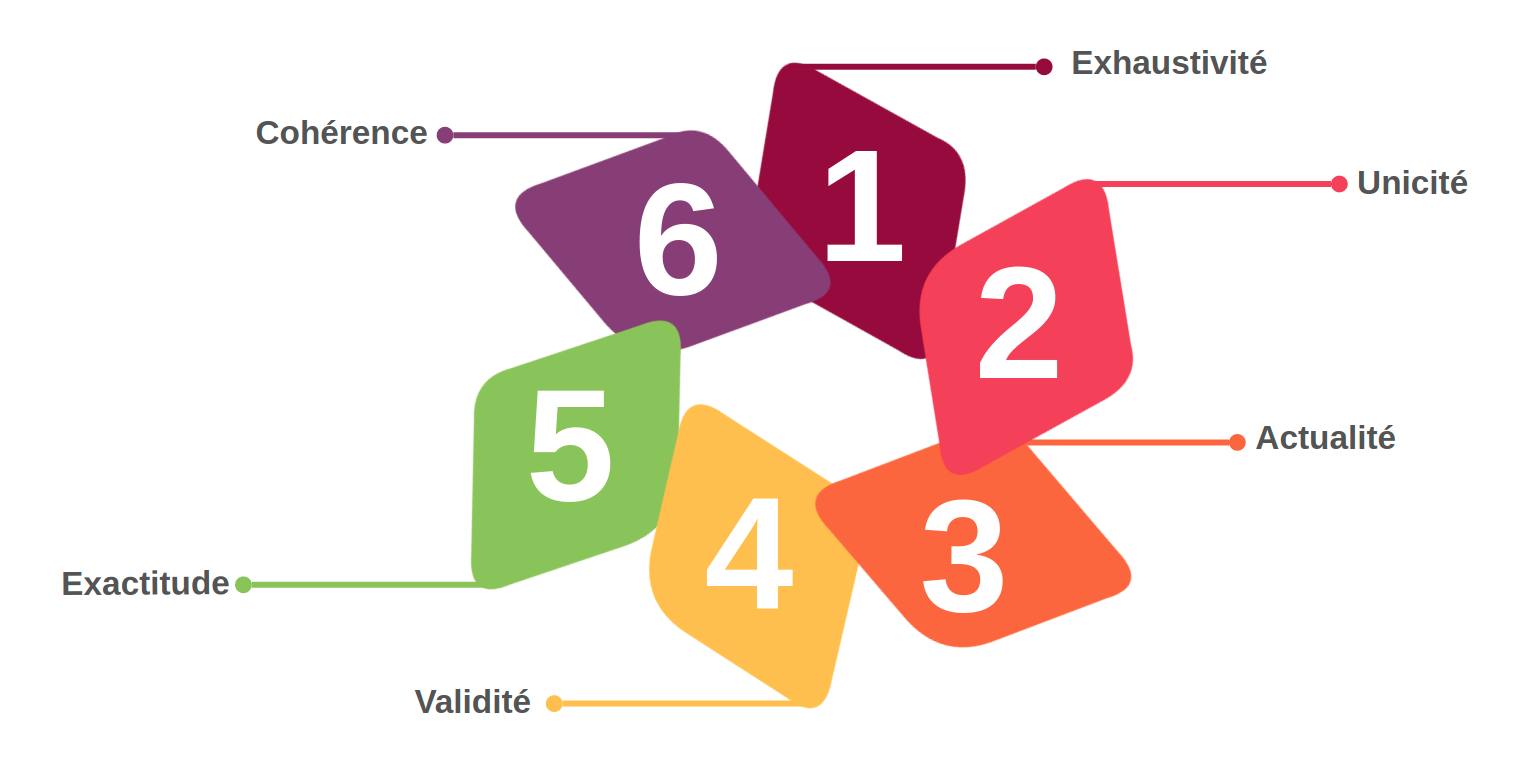
\includegraphics[scale=0.33]{Static/Dim3.png} 
  \end{center}
\end{figure}

\end{enumerate}
\vspace {0.5cm}

Dans une tentative de synth\`ese, Berti-Equille \cite{BertiEquille2004} fait remarquer en 2004 que quel que soit le domaine d’application, les mesures de qualité de données les plus fréquemment mentionnées, sont l'exactitude, la complétude, l’actualité et la cohérence. Mais nous retiendrons pour cette \'etude les six dimensions susmentionn\'ees.

\subsubsection{\textbf{Dimensions de la qualit\'e des donn\'ees \`a l'\`ere du \textit{big data}}}

De nos jours, les \textit{big data} imposent de nouveaux défis liés à leurs principales caractéristiques. En particulier, afin d'aborder les questions de volume et de vélocité, il est nécessaire de repenser les méthodes d'évaluation pour exploiter les scénarios de calcul parallèle. Mais aussi, il revient de se demander si les dimensions de qualit\'e existantes sont toujours d'actualit\'e ou n\'ecessitent des ajustements. Ainsi, pour \'evaluer la qualit\'e des \textit{big data}, Cai et Zhu \cite{Cai_Zhu_2015} proposent une hi\'erarchie de dimensions et de sous-dimensions: 
\begin{itemize}

\item[>] la \textbf{disponibilit\'e} de la donn\'ee caract\'eris\'ee par:
\begin{itemize}[parsep=0cm,itemsep=0cm]
\item l'accessibilit\'e:  existe-t-il des facilit\'es d'acc\`es aux donn\'ees?; 
\item l'actualit\'e: la donn\'ee est-elle r\'eguli\`erement mise \`a jour?;
\item l'autorisation: a-t-on le droit d'utiliser ces donn\'ees? a-t-on les acc\`es n\'ecessaires ?;
\end{itemize}
%\vspace {0.5cm}

\item[>] l'\textbf{utilisabilit\'e}  de la donn\'ee caract\'eris\'ee par:
\begin{itemize}[parsep=0cm,itemsep=0cm]
\item l'existence d'une documentation;
\item la cr\'edibilit\'e : qui concerne la fiabilit\'e de la source de donn\'ees, la normalisation des donn\'ees et le moment o\`u les donn\'ees sont produites;
\item l'existence de m\'eta-donn\'ees;
\end{itemize}
%\vspace {0.5cm}

\item[>] la \textbf{fiabilit\'e} de la donn\'ee caract\'eris\'ee par quatre des six dimensions identifiées par la \acrshort{dama} \cite{dama}:
\begin{itemize}[parsep=0cm,itemsep=0cm]
\item l'exactitude;
\item l'int\'egrit\'e ou validit\'e \cite{dama} ;
\item la coh\'erence;
\item la compl\'etude;
\item l'auditabilit\'e : l'auditabilité signifie que l'exactitude et l'intégrité des données  peuvent être évaluer équitablement dans des limites de temps et de main-d'œuvre rationnelles ;
\end{itemize}
%\vspace {0.5cm}

\item[>] la \textbf{pertinence} de la donn\'ee caract\'eris\'ee par:
\begin{itemize}
\item l'aptitude de la donn\'ee \`a satisfaire son utilisateur;
\end{itemize}
%\vspace {0.5cm}

\item[>] la \textbf{qualit\'e de la pr\'esentation} caract\'eris\'ee par:
\begin{itemize}[parsep=0cm,itemsep=0cm]
\item la lisibilit\'e : est-ce que la donn\'ee est bien d\'efinie suivant une terminologie connue et courante ?;
\item la structuration : la structure fait référence \`a la difficulté à transformer les données semi-structurées ou non structurées en données structurées.
\end{itemize}
\newpage
\begin{figure}[!h]
  \caption{Hiérarchisation des dimensions selon Cai et Zhu}  \label{fig:cai_shu}
  \begin{center}
    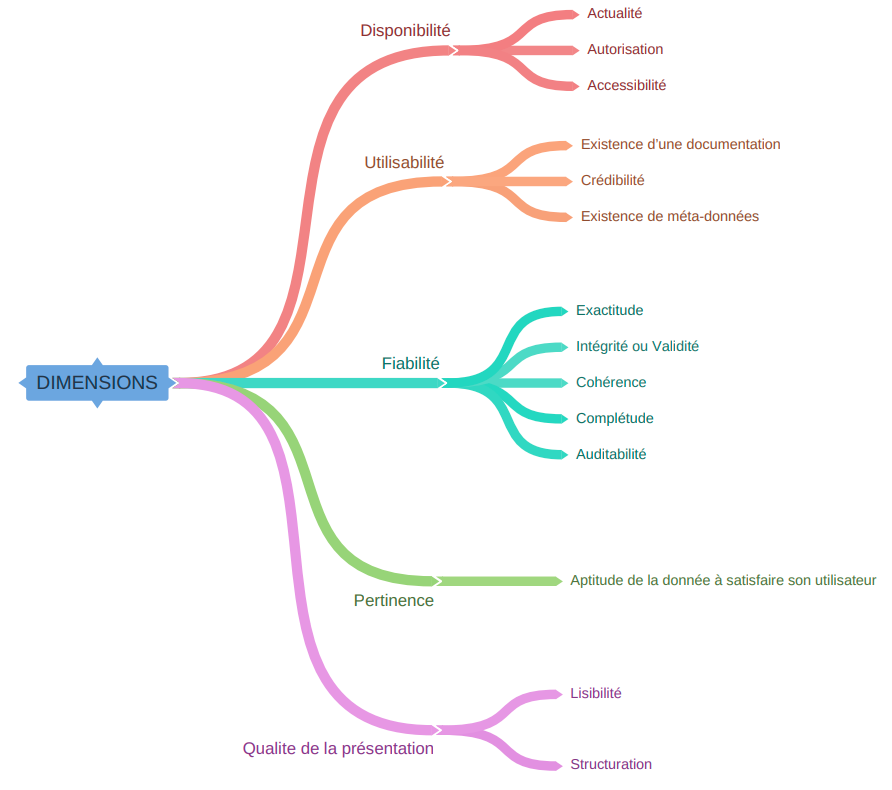
\includegraphics[scale=0.6]{Main/Static/Dimensions_Screen.png} 
  \end{center}
\end{figure}

\end{itemize}  
%\vspace{0.5cm}

Plusieurs autres auteurs ont \'egalement propos\'e des cadres m\'ethodologiques d'analyse de la qualit\'e des \textit{big data}. Ramasamy et Chowdhury \cite{articleRamasamyChowdhury2020} en font une pr\'esentation succincte r\'esum\'e. En plus de l'accessibilit\'e \cite{Cai_Zhu_2015}, la lisibilit\'e \cite{Cai_Zhu_2015}, la cr\'edibilit\'e et la confiance \cite{articleRamasamyChowdhury2020} (la cr\'edibilit\'e \cite{Cai_Zhu_2015}), la coh\'esion \cite{articleRamasamyChowdhury2020} (la coh\'erence \cite{dama}, \cite{Cai_Zhu_2015}) ainsi que la confidentialit\'e \cite{articleRamasamyChowdhury2020} (l'autorisation \cite{Cai_Zhu_2015}), ils font ressortir quatre autres dimensions jug\'ees importantes : 

\begin{itemize}[parsep=0cm,itemsep=0cm]
\item le p\'edigr\'ee ou la lignée : cette dimension permet de connaître la source des donn\'ees afin d'y corriger les éventuelles incoh\'erences ;
\item la capacit\'e d'analyse en temps r\'eel;
\item la redondance :  elle fait r\'ef\'erence \`a la capacit\'e \`a repr\'esenter le monde r\'eel sans r\'ep\'etition des informations ;
\item le volume : cette dimension permet d'analyser le volume des donn\'ees extraites.

\end{itemize}
\vspace {0.5cm}

Au regard des dimensions \'enum\'er\'ees, on constate que plusieurs d'entre elles int\`egrent le fait que les \textit{big data} ne sont pas forc\'ement produites en entreprise, mais pour la plupart proviennent de sources externes et que cela a un impact sur la qualit\'e. Ainsi, on peut distinguer des dimensions qui sont quantifiables et d'autres ayant un aspect plus qualitatif. On retiendra néanmoins que les dimensions retenues pour les donn\'ees structur\'ees demeurent quand m\^eme applicables dans le contexte des \textit{big data}.
%Mettre en place des indicateurs de performance pour piloter la qualité des données est un acte fondateur témoignant du sérieux de l’entreprise dans sa démarche. C’est  une condition du succès, comme nous le rappelle Thierry Savit :
%Before attempting to use data quality dimensions, an organisation needs to agree the quality rules against which the data needs to be assessed against. 
%nous allons donc dans un premier temps pr\'esenter les dimensions qui ont inspir\'e celles impl\'ement\'ees.

\subsubsection{\textbf{Outils d'\'evaluation de la qualit\'e des donn\'ees}}
L'\'evaluation de la qualit\'e suivant les diff\'erentes dimensions retenues par l'entreprise, ne peut se faire efficacement de façon manuelle. Elle nécessite l'utilisation d'un outil ou d'une plateforme sp\'ecialement d\'edi\'e \`a cette t\^ache. Trois (3) options s'offrent aux entreprises \cite{linkedinDeepakRout}:
\begin{description}[parsep=0cm,itemsep=0cm]
\item[un outil fait maison:] cette approche requiert un énorme investissement en terme de travail afin de mettre en place un outil facilement adapt\'e aux diff\'erentes sources de donn\'ees; mais offre tous les avantages li\'es \`a la disposition d'un outil personnalis\'e et facilement maintenable. Elle convient aux grandes organisations disposant d'une grosse \'equipe de d\'eveloppement rompue \`a cette t\^ache;
\item[un outil open source: ] il s'agit de l'approche la plus courante. La gratuité, la connectivité avec la majorit\'e des environnements de données modernes ainsi que la disponibilité des fonctionnalités nécessaires en font un choix de premier ordre. Les plus populaires sont: Apache Griffin, Deequ, Great Expectations, MobyDQ, Data Validator, Bigdata Profiler.
\item[une solution commerciale: ] elles sont pour la plupart d\'evelopp\'ees par des fournisseurs de solutions \acrfull{etl}. Et conviennent mieux aux organisations ayant déjà souscrit \`a un produit en provenance de la m\^eme entreprise. Elles offrent l'avantage d'avoir un support technique et une int\'egration transparente avec l'\acrshort{etl} en d\'epit du co\^ut des licences. Quelques exemples de ces produits sont les offres de Talend (Talend Data Quality) et Informatica (Talend Data Quality). 
\end{description}
%\begin{landscape}

Nous nous intéressons particuli\`erement aux solutions open source, plus précisément \`a Apache Griffin. Nous pr\'esentons un rapide comparatif des outils les plus en vue du march\'e.

%\begin{footnotesize}

\begin{table}[H]
\caption{Comparaison de Apache Griffin - Great Expectations - Deequ}
\footnotesize
%\begin{adjustwidth}{-3em}{-1em}%{-4em}{-1em}small
\vspace{0.5cm}
\begin{tabular}{ll|cl|cl|cl}%>{\justify}p{3cm}>{\justify}p{3cm}>{\justify}p{3cm}
\toprule 
                          && \textbf{Apache Griffin}     && \textbf{Great Expectations}     && \textbf{Deequ}               \\%& mobyDQ & data-validator & bigdata-profiler  \\
\midrule
%\rowcolor{lightgray}

                          && Pr\'ed\'efinies     && Pr\'ed\'efinies         && Pr\'ed\'efinies        \\%& Pr\'ed\'efinie (faible vari\'et\'e) & Pr\'ed\'efinie & Pr\'ed\'efinie \\
\textbf{R\`egles}                  && et personnalisables  && (Riches et vari\'ees)  && (Riches et vari\'ees)         \\%& Pr\'ed\'efinie (faible vari\'et\'e) & Pr\'ed\'efinie & Pr\'ed\'efinie \\
\textbf{de qualit\'e}              &&  en utilisant      &&  et personnalisables     && Comp\'etences en          \\%& Pr\'ed\'efinie (faible vari\'et\'e) & Pr\'ed\'efinie & Pr\'ed\'efinie \\
                          &&  du SQL            &&    (Python)            && Scala \\%& Pr\'ed\'efinie (faible vari\'et\'e) & Pr\'ed\'efinie & Pr\'ed\'efinie \\
\hline 
\textbf{Profiling}                 && Manuel             && Automatique            && Automatique               \\%& - & - & -\\ 

\hline
\textbf{Suggestions}               && Non                && Oui                    && Oui                         \\%& Non & Non & Non\\ 
\textbf{de r\`egles }              &&                    &&                        &&                              \\%& Non & Non & Non\\ 

\hline
\textbf{Stockage des}              && Elasticsearch,HDFS && JSON                   && Configurable                  \\%& PostgreSQL & - & DogStatsD\\ 
\textbf{m\'etriques}               && Personnalisable    &&                        && Spark DataFrame                               \\%& PostgreSQL & - & DogStatsD\\ 

\hline
\textbf{D\'etection d'anomalies}    && Pas encore         && Non                    && Oui                              \\%& Non & Non & Non\\ 

\hline 
\textbf{Documentation automa-}             &&                    &&                        &&                                   \\%& IU & - & -\\ 
\textbf{tique des m\'etriques/}          && IU                 && Documentation          && -                                  \\
\textbf{Interface Utilisateur(IU)}     &&                    &&                        &&                                     \\

\hline 
\textbf{}                    && JDBC,Avro,Hive        && SGBDR,                 && Toutes sources                       \\%&  & Hive, OrcFile,Parquets & CSV,JSON,Parquet\\ 
 \textbf{Source de donn\'ees}                       && Hadoop,Fichiers plat,    &&S3                      && support\'ees                         \\%&  & Hive, OrcFile,Parquets & CSV,JSON,Parquet\\ 
\textbf{}                 && Personnalisable       &&Fichiers plat              && par Spark                            \\%&  & Hive, OrcFile,Parquets & CSV,JSON,Parquet\\ 

\hline 
\textbf{Langage}                   && Scala              && Python                 && Scala                       \\%& Python & Scala & Scala\\ 
                          &&\& SQL              &&                        && \& Interface Python          \\%& Python & Scala & Scala\\ 

\hline 
\textbf{Support technique/}        && Apache             && Professionnel          && AWS                           \\%& Ubisoft & - & - \\ 
\textbf{communaut\'e }             &&                    &&  et communaut\'e       &&                                \\%& Ubisoft & - & - \\ 

\hline 
\textbf{Documentation}             && D\'etaill\'ee      && D\'etaill\'ee          && D\'etaill\'ee                   \\%& D\'etaill\'ee  & Minimaliste  & Pauvre \\

\hline 
\textbf{Volume de donn\'ees}       && Petaoctet         && Gigaoctet              &&  -                             \\%& D\'etaill\'ee  & Minimaliste  & Pauvre \\ 

\hline 
\textbf{API}                       && Oui                && Non                    && Non                                \\%& D\'etaill\'ee  & Minimaliste  & Pauvre \\ 

\hline 
\textbf{Environnement}             && Hadoop             && Pandas,SQL,BigQuery    &&                                  \\%& D\'etaill\'ee  & Minimaliste  & Pauvre \\ 
\textbf{d'ex\'ecution}             && Spark              && Redshift, Spark, mais  && Spark                             \\%& D\'etaill\'ee  & Minimaliste  & Pauvre \\ 
                          && Hive               && optimis\'e pour Python &&                                   \\%& D\'etaill\'ee  & Minimaliste  & Pauvre \\ 

\hline 
\textbf{Alerte}                    && Email              && Email/Slack 			&&                                    \\%& D\'etaill\'ee  & Minimaliste  & Pauvre \\ 

\hline 
\textbf{Modes}                     && Batch et Streaming && Batch                  && Batch                               \\%& D\'etaill\'ee  & Minimaliste  & Pauvre \\ 

\hline 
\textbf{Ex\'ecution}               && Oui                && Apache                 &&                                      \\%& D\'etaill\'ee  & Minimaliste  & Pauvre \\ 
\textbf{programm\'ee}              && crontab            && Airflow                &&                                      \\%& D\'etaill\'ee  & Minimaliste  & Pauvre \\ 

\bottomrule
\end{tabular}
%\end{adjustwidth}

\end{table}
%\end{footnotesize}
%\end{landscape}

%\newpage

\begin{table}[H]
\caption{Comparaison de mobyDQ - data-validator - bigdata-profiler}

%\begin{adjustwidth}{-1em}{-2em}%{-1em}{-2em}small
\vspace{0.5cm}
\footnotesize
\setlongtables
\begin{longtable}{ll|cl|cl|cl}%>{\justify}p{3cm}>{\justify}p{3cm}>{\justify}p{3cm}
\toprule 

                                         &&  \textbf{mobyDQ}               && \textbf{data-validator}   && \textbf{bigdata-profiler}                     \\
\midrule
\endhead
                                         && 	Pr\'ed\'efinies	           &&                           && N\'ecessite des                      \\%
\textbf{R\`egles}                        &&    mais faible                 && Pr\'ed\'efinies           && comp\'etences en                     \\
\textbf{de qualit\'e}                    &&   vari\'et\'e                  && (Riches et vari\'ees)     && programmation                        \\
                                         &&  de r\`egles                   &&                           && scala                                \\
\hline 

\textbf{Profiling}                       && Non                            && Non                       && Non                                  \\%& - & - & -\\ 
\hline

\textbf{Suggestions}                     && Non                            && Non                       && Non                                  \\%& Non & Non & Non\\ 
\textbf{de r\`egles}                     &&                                &&                           &&                                      \\%& Non & Non & Non\\ 
\hline

\textbf{Stockage des}                    &&PostgreSQL                      && JSON                      && DogStatsD                            \\%& PostgreSQL & - & DogStatsD\\ 
\textbf{m\'etriques}                     &&                                &&                           &&                                      \\%& PostgreSQL & - & DogStatsD\\ 
\hline

\textbf{D\'etection d'anomalies }         && Non                            && Non                       && Oui                                  \\%& Non & Non & Non\\ 
\hline 

\textbf{Documentation automa-}                   &&                                &&                           &&                                      \\%& IU & - & -\\ 
\textbf{tique des m\'etriques}                 && IU                             && Aucun                     && Aucun                                \\
\textbf{Interface Utilisateur(IU)}       &&                                &&                           &&                                      \\
\hline 

                                         && SGBDR,Snowflake                && OrcFile,                  && CSV,                       \\%&  & Hive, OrcFile,Parquets & CSV,JSON,Parquet\\ 
\textbf{Source de donn\'ees}             && Impala,Teradata                && Parquet,                  && Parquet,                         \\%&  & Hive, OrcFile,Parquets & CSV,JSON,Parquet\\ 
                                         && Hive                           && Hive                      && JSON                            \\%&  & Hive, OrcFile,Parquets & CSV,JSON,Parquet\\ 
\hline 

\textbf{Langage}  						 && Python                         && Scala                     && Scala                                \\%& Python & Scala & Scala\\ 
\hline 

\textbf{Support technique/}              && Ubisoft                        &&                           &&                                      \\%& Ubisoft & - & - \\ 
\textbf{communaut\'e}                    &&                                &&                           &&                                      \\%& Ubisoft & - & - \\ 
\hline 

\textbf{Documentation}                   && D\'etaill\'ee                  && Minimaliste               && Pauvre                               \\%& D\'etaill\'ee  & Minimaliste  & Pauvre \\
\hline 
 
\textbf{Volume de donn\'ees}             && -                              && -                         && -                                    \\%& D\'etaill\'ee  & Minimaliste  & Pauvre \\ 
\hline 

\textbf{API}                             && Oui                            && Non                       && Non                                  \\%& D\'etaill\'ee  & Minimaliste  & Pauvre \\ 
\hline 

\textbf{Environnement}                   &&  Nginx                         &&                           &&                                      \\%& D\'etaill\'ee  & Minimaliste  & Pauvre \\ 
\textbf{d'ex\'ecution}                   &&  Python                        && Spark                     && Spark                                \\%& D\'etaill\'ee  & Minimaliste  & Pauvre \\ 
                                         &&  GraphQL                       &&                           &&                                      \\%& D\'etaill\'ee  & Minimaliste  & Pauvre \\ 
\hline 

\textbf{Alerte}                          && Email                          && Email                     && Non                                  \\%& D\'etaill\'ee  & Minimaliste  & Pauvre \\ 
\hline 

\textbf{Modes}                           && Batch                          && Batch                     && Batch                                \\%& D\'etaill\'ee  & Minimaliste  & Pauvre \\ 
\hline 

\textbf{Ex\'ecution}                     && Non                            && Oui                       && Possible                                   \\%& D\'etaill\'ee  & Minimaliste  & Pauvre \\ 
\textbf{programm\'ee}                    &&                                && crontab                   &&                                      \\%& D\'etaill\'ee  & Minimaliste  & Pauvre \\ 
\bottomrule
\end{longtable}
%\end{adjustwidth}

\end{table}
%\newpage
\subsection{Anomalies et Mesures correctives}
\subsubsection{\textbf{Diff\'erents types d'anomalies}}

Les données jouent un r\^ole crucial pour prendre les bonnes décisions à propos de la direction future de l’entreprise, et comme le dit l'adage \textit{«\`a données inexactes, résultats erronés»}. Les anomalies dans les données sont très variées et sont causées par plusieurs facteurs. Dans \cite{IFP}, on retrouve cinq (5) des probl\`emes les plus courants en mati\`ere de qualit\'e des donn\'ees. De son c\^ot\'e, Ben Salem \cite{bensalem}  met en évidence huit (8) classes d'anomalies dans les donn\'ees regroupant aussi bien les r\'esultats de \cite{IFP} que ceux de Todoran \cite{todoran}. Essentiellement nous avons: 

\begin{itemize}[parsep=0cm,itemsep=0cm]
\item \textbf{l'incohérence des formats, la codification des donn\'ees, la multiplicit\'e des langues et des unit\'es de mesures} : on d\'esigne ici l'existence de formatages diff\'erents pour la m\^eme donn\'ee; par exemple la date aux formats JJ/MM/AAAA et MM/JJ/AAAA, le format des donn\'ees de type num\'erique doit \^etre clairement pr\'ecis\'e. Comme pour le formatage, les différences de langue, d'alphabet ou d'unités de mesure peuvent g\'en\'erer des erreurs (caractères sp\'eciaux;  fahrenheit ou celsius);

\item \textbf{les valeurs erronées, les valeurs aberrantes (commun\'ement appel\'ees \textit{outliers})}: ce type d'anomalie est le plus souvent rencontré. Un \textit{outlier} est une valeur qui est anormale par rapport au comportement des autres valeurs. Une valeur erronée d\'esigne en revanche une valeur diff\'erente de celles attendues. Elles sont parfois difficiles \`a d\'etecter surtout si le formatage reste acceptable;

\item \textbf{les donn\'ees incompl\`etes ou valeurs manquantes}: elles se manifestent par l'absence partielle ou totale d'informations pertinentes (ou non), laissant place \`a des champs partiellement remplis ou laiss\'es blancs. Todoran \cite{todoran}, fait remarquer que les données incomplètes repr\'esentent un type d'imperfection qui affecte surtout les bases de données volumineuses. Elles ne sont pas toutes de même nature. On distingue selon la classification faite par Little et Rubin (1987) cit\'e par Glasson-Cicognani et Berchtold \cite{glassoncicognani}, les :
\begin{itemize}[parsep=0cm,itemsep=0cm]
\item \acrfull{mcar}: les donn\'ees manquantes sont qualifi\'ees de \acrshort{mcar}  lorsqu'il n'est pas possible de d\'efinir un profil propre aux individus pr\'esentant cette absence dans les donn\'ees (donn\'ees manquantes complètement aléatoires);
\item \acrfull{mar}:  il est question cette fois de donn\'ees manquantes al\'eatoires. Les donn\'ees manquantes sont dites \acrshort{mar} lorsque leur probabilit\'e d'apparition d\'epend des valeurs non manquantes prises pas les autres variables;
\item \acrfull{mnar}: les donn\'ees manquantes sont \acrshort{mnar}, lorsque la probabilit\'e d'absence de la donn\'ee d\'epend de la variable en question. C'est le cas par exemple où des individus ayant un revenu important refuse de le d\'evoiler;
\end{itemize}

\item \textbf{la duplication des donn\'ees}: les données dupliquées sont un problème que toutes les entreprises devront traiter. Ben Salem \cite{bensalem}, parle au sens plus large de redondance, y ajoutant ainsi la notion de similarit\'e entre les lignes. Son évaluation n\'ecessite un calcul de similarit\'e entre les donn\'ees. Plusieurs m\'ethodes de calcul de distance de similarit\'e sont pr\'esentes dans la litt\'erature;

\item \textbf{les donn\'ees impr\'ecises, les valeurs par d\'efaut} : une donn\'ee impr\'ecise d\'epeint la situation dans laquelle il y a des difficult\'es \`a identifier la vraie valeur de la donn\'ee: par exemple la temp\'erature par d\'efaut peut \^etre mise \`a z\'ero (0) mais aussi z\'ero peut \^etre la valeur r\'eelle;

\item \textbf{l'obsolescence des donn\'ees}: deux aspects ici sont concern\'es, l'actualit\'e de la donn\'ee vis-\`a-vis d'une r\'ef\'erence et l'anciennet\'e de la donn\'ee;

\item \textbf{les d\'ependances} :  il s'agit  des d\'ependances entre attributs, qui sont viol\'ees ou qui doivent \^etre mat\'erialis\'ees. 
\end{itemize}

\subsubsection{\textbf{Mesures d'am\'eliorations}} 
La qualité des données est évaluée afin de d\'eterminer si la donnée est appropriée pour une utilisation spécifique, mais aussi dans le but d'établir les processus nécessaires à son amélioration. Ces processus ne devraient donc pas être exclusivement basées sur la correction des données, mais devraient également pr\'evenir l'introduction de donn\'ees erron\'ees. 
\\

En termes de corrections, plusieurs mesures et algorithmes peuvent \^etre appliqu\'es, en fonction du type d'anomalie d\'etect\'e. Pour le traitement des valeurs manquantes deux approches sont privil\'egi\'ees \cite{glassoncicognani}. On peut soit les omettre de l'analyse ou dans la suite du processus, soit proc\'eder \`a une imputation. La premi\`ere approche consiste \`a ne consid\'erer que  les observations qui ne contiennent aucune donn\'ee manquante. C'est la plus courante d'ailleurs. On pourrait appliquer cette m\'ethode si le taux de valeurs manquantes n'exc\`ede pas 5\% \cite{datascience}. L'imputation quant-\`a-elle, est une technique qui consiste \`a remplacer la valeur manquante par une valeur plausible. Il existe plusieurs m\'ethodes d'imputations. Biernat et Lutz (2015) \cite{datascience}, identifient quelques unes d'entre elles :

\begin{itemize}[parsep=0cm,itemsep=0cm]
\item l'imputation par r\`egle: lorsqu'elle est connue, on peut se servir d'une r\`egle m\'etier pour g\'en\'erer la valeur manquante;

\item l'imputation par la moyenne, la m\'ediane ou le mode: il s'agit de calculer ces diff\'erentes statistiques sur les donn\'ees observ\'ees afin de les substitu\'ees aux valeurs manquantes;

\item l'imputation par r\'egression : l'imputation est r\'ealis\'e en d\'eterminant la valeur manquante par la valeur pr\'edite par le mod\`ele de r\'egression (r\'egression locale, r\'egression lin\'eaire, r\'egression \textit{Partial Least Squares}, ...);

\item l'imputation par \textit{hot-deck} ou \textit{cold-deck} : on tire al\'eatoirement avec remise une valeur parmi l’ensemble des individus ayant une valeur observée pour la variable d’intérêt, afin de remplacer la valeur manquante. Ce tirage peut \^etre fait directement dans le jeu de donn\'ees analys\'e (\textit{hot}) ou dans une source de donn\'ees externe (\textit{cold});

\item la m\'ethode des plus proches voisins : elle consiste à exécuter l’algorithme des k plus proches voisins afin de modéliser et de prévoir les données manquantes;

\item l'imputation par utilisation des forêts aléatoires : cette méthode nécessite une première imputation naïve (par défaut une complétion par la moyenne), afin d’obtenir un échantillon d’apprentissage complet. Puis une série de forêts aléatoires sont ajustées jusqu’à la première dégradation du modèle \cite{wikistat-dm};

\item l'imputation multiple: l’imputation multiple consiste, comme son nom l’indique, à imputer plusieurs fois les valeurs manquantes afin de combiner les résultats pour diminuer
l’erreur (le bruit) due à une imputation simple. Elle est basés sur l'échantillonnage \textit{bootstrap}, et donne des r\'esultats semblables \`a ceux de l'algorithme \acrfull{em}. Cette m\'ethode est une bonne alternative en cas de donn\'ees manquantes \acrshort{mar} ou \acrshort{mcar}. Elle offre l'avantage de ne pas modifier significativement les relations entre les variables.
\end{itemize}
Pour ce qui est des valeurs aberrantes ou erron\'ees, Biernat et Lutz \cite{datascience} proposent l'utilisation de m\'ethodes d'imputations afin de corriger ces diff\'erentes anomalies lorsqu'elles sont av\'er\'ees. \\

Les donn\'ees manquantes et aberrantes ne sont pas les seules anomalies qui minent la qualit\'e , nous avons \'egalement le ph\'enom\`ene de duplication. Face \`a elle, deux solutions se pr\'esentent: on peut supprimer syst\'ematiquement les donn\'ees en double ou alors proc\'eder \`a une d\'eduplication. La suppression des donn\'ees en double, n\'ecessite au préalable l'identification d'un crit\`ere d'unicit\'e. Le processus de d\'eduplication quant \`a lui, se fait essentiellement en cinq (5) \'etapes  \cite{bensalem}: 

\begin{enumerate}[parsep=0cm,itemsep=0cm]
\item le choix des attributs cl\'es de dédoublonnage ;
\item le choix d’un algorithme de similarité: la similarité des données est définie comme étant la distance entre deux valeurs, de même type, de deux enregistrements. Plusieurs algorithmes (mesures lexicographiques, mesures phonétiques,...) sont propos\'es en fonction du contexte et de la donn\'ee (chaînes de caractères, données numériques,dates). 
\item le choix d'une approche de correspondance (\textit{Match}): cette \'etape permet de sélectionner l'algorithme \`a mettre en place pour savoir si deux ou plusieurs enregistrements sont similaires. Elle pr\'epare la phase de fusion. ;

\item le choix de la strat\'egie de fusion des \textit{tuples} similaires (\textit{Merge}): la fusion permet de créer un "enregistrement-résultat" plus riche, contenant plus d'informations;

\item l'\'elimination et l'\'evaluation du taux d'\'elimination des similaires et des doublons.

\end{enumerate}

En ce qui concerne, les erreurs relatives \`a une incohérence des formats ou des anomalies dans la codification des données ou des unités de mesure, des corrections peuvent \^etre faites en \'etablissant des r\`egles ou un arbre de choix. L'utilisation des r\`egles m\'etiers et des arbres de choix sont \'egalement privil\'egi\'ees pour les corrections en cas de violations des d\'ependances entre attributs.
\\

Mais toutes ces mesures ne sont applicables qu'apr\`es la survenue de l'anomalie. Afin d'am\'eliorer efficacement la qualit\'e des donn\'ees, une approche processus doit \^etre \'egalement mise en place. L’approche processus a pour objectif de prévenir l’introduction de données erronées. Elle peut int\'egrer une d\'eduplication interactive, une validation interactive ainsi que la mise en place de contraintes ou de r\`egles fortes afin d'éviter la survenue de certaines non conformités. De plus, l'am\'elioration de la qualit\'e est une d\'emarche continue et it\'erative. Elle commence par une validation du niveau de qualit\'e sur les donn\'ees existantes. Ensuite nous avons: la d\'efinition d'un niveau de qualit\'e cible, l'atteinte et le maintien de ce niveau \`a travers le traitement des diff\'erentes anomalies, puis le contr\^ole de la qualit\'e des donn\'ees.

\section*{Conclusion}
La qualit\'e des donn\'ees est le degr\'e auquel un ensemble de caract\'eristiques propres aux donn\'ees (complétude, unicité, actualit\'e, validit\'e, exactitude et coh\'erence) répond aux exigences de l'utilisation pr\'evue. Son \'evaluation nécessite l'usage d'une plateforme entièrement d\'edi\'ee   \`a cette  tâche. Cette derni\`ere doit pouvoir r\'epondre aux exigences de rapidit\'e et de mall\'eabilit\'e de l'organisation. En fonction des anomalies d\'etect\'ees dans les donn\'ees des mesures d'am\'eliorations sp\'ecifiques peuvent \^etre mises en place. Ce chapitre met fin \`a la pr\'esentation contextuelle et  th\'eorique du sujet. Le chapitre suivant amorce la pr\'esentation des r\'esultats \`a travers la présentation d'Apache Griffin ainsi que les configurations faites.


%\Partie 2
\part{\normalfont \LARGE PR\'ESENTATION DES R\'ESULTATS}
%Chapitre3
\chapter{Results presentation}

\section{Pr\'esentation de Apache Griffin}


\subsection{Aperçu de l'outil}
Apache Griffin, est une solution open source de qualit\'e des donn\'ees pour le \textit{big data}. Il est d\'ecrit par ses concepteurs comme \'etant une plateforme offrant des services de qualit\'e des donn\'ees. De ce fait, il fournit un cadre complet d'analyse, permettant de r\'ealiser diverses t\^aches telles que la d\'efinition d'un mod\`ele de qualit\'e des donn\'ees, le calcul de diverses m\'etriques, l'automatisation de la validation des donn\'ees ainsi qu'une visualisation unifiée des m\'etriques. Gr\^ace aux infrastructures composant son \'ecosyst\`eme, Apache Griffin (Griffin) permet de g\'erer des donn\'ees venant aussi bien en temps r\'eel (\textit{streaming}) que par lot (\textit{batch}), tout en relevant les d\'efis en mati\`ere de qualit\'e dans les applications \textit{big data}. Face \`a l'absence de consensus sur la qualit\'e, Apache Griffin propose un standard sans pour autant \^etre restrictif.
\\

Conçu dans les locaux d'eBay en Mars 2016, puis confi\'e \`a la fondation Apache le 7 D\'ecembre de la m\^eme ann\'ee, Apache Griffin venait combler un certain nombre de besoins notamment \cite{ApacheGriffinIntro} : 
\begin{itemize}[parsep=0cm,itemsep=0cm]
\item le suivi de la qualit\'e  depuis de multiples sources de donn\'ees jusqu'aux applications cibles, tout en tenant compte de leurs historiques;

\item l'\'evaluation de la qualit\'e des donn\'ees en \textit{streaming} et en \textit{batch} tout en offrant la possibilit\'e de suivre l'évolution des diff\'erentes m\'etriques;

\item la mise en place d'une plateforme exposant une \acrshort{api}, permettant aux développeurs d'impl\'ementer leur propre interface utilisateur.
\end{itemize}

\subsection{Fonctionnalit\'es  d'Apache Griffin}

Afin de satisfaire ces diff\'erents besoins, Apache Griffin propose de nombreuses fonctionnalit\'es. Telles que pr\'esent\'ees dans la documentation, nous avons: 

\begin{itemize}[parsep=0cm,itemsep=0cm]

\item \textbf{la d\'efinition de mesures} : l'exactitude, l'exhaustivité ou la compl\'etude, l'actualité, l'unicité, la validité, la cohérence; il s'agit des diff\'erentes dimensions de la qualit\'e des donn\'ees qui peuvent \^etre \'evalu\'ees. L’utilisateur peut créer, modifier, supprimer et planifier des jobs pour les données venant par batch ;

\item \textbf{la surveillance des anomalies} : l'\'etablissement d'attentes sp\'ecifiques pour détecter les données anormales, tout en offrant la possibilit\'e de les téléchargés  ;

\item \textbf{les alertes en cas de d\'etection d'anomalies} : signaler les problèmes de qualité des données par e-mail ou sur la plateforme;

\item \textbf{la surveillance visuelle} : gr\^ace \`a son interface web, on peut appr\'ecier l'\'etat de la qualité des données au fil du temps;

\item \textbf{le temps réel} : l'inspection de la qualité des données peut être effectuée en temps réel;

\item \textbf{l'\'elasticit\'e et l'agilit\'e} : gr\^ace \`a ses facult\'es, Griffin peut être utilisé pour l'analyse des données provenant de plusieurs entrepôts de données. De plus, il fonctionne dans un environnement (Spark et Hadoop) pouvant g\'erer de grands volumes de donn\'ees (1,2 Petaoctet soit 1000 T\'eraoctet, cas d'eBay);

\item \textbf{la simplicit\'e} : Griffin fournit une interface utilisateur simple et facile à utiliser qui peut gérer les données et les règles de qualité; en même temps, les utilisateurs peuvent visualiser les résultats de qualité des données et personnaliser le contenu de l'affichage par le biais du panneau de contrôle.

\end{itemize}

\begin{figure}[H]
  \caption{Fonctionnalit\'es de Apache Griffin}  \label{fig:xray}
  \begin{center}
    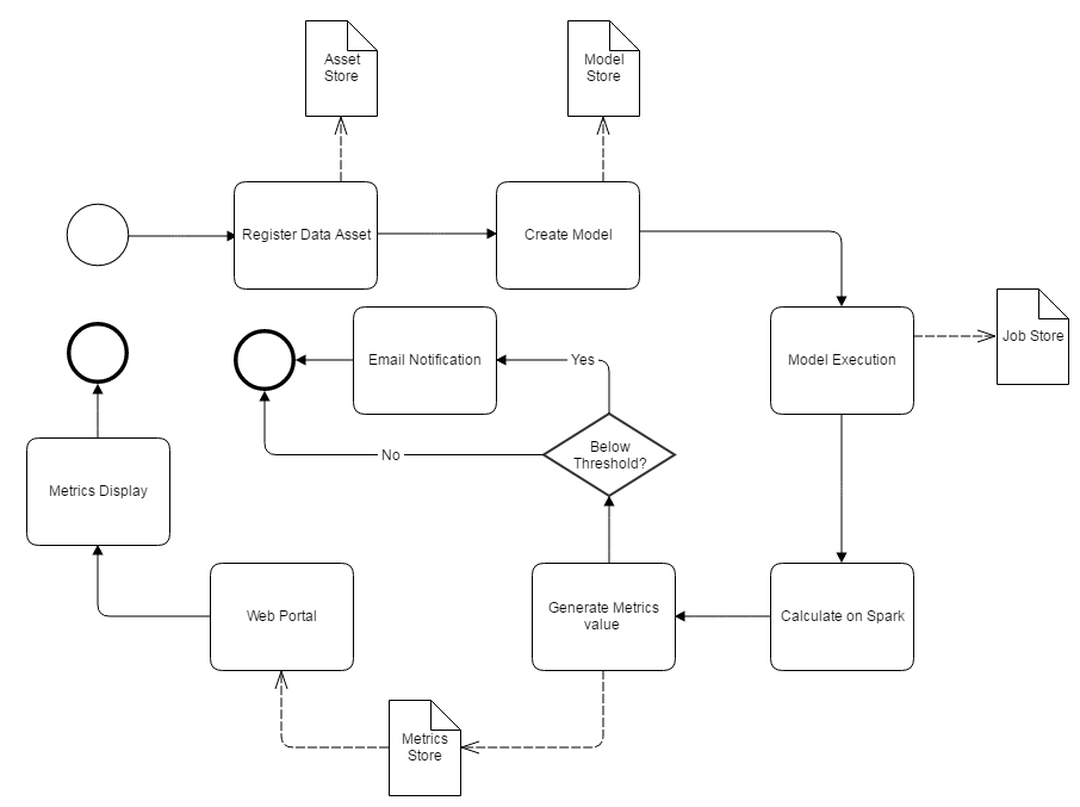
\includegraphics[scale=0.45]{Static/Capture.png} 
  \end{center}
\end{figure}

\subsection{Dimensions de la qualit\'e de donn\'ees}
 Dans cette sous-section, nous mettrons l'accent sur les langages de qualit\'e des donn\'ees de Griffin et sur les dimensions impl\'ement\'ees. En effet, les règles de qualit\'e des donn\'ees de Griffin sont \'edit\'ees soit \`a l'aide de  \emph{griffin-dsl} ou du \emph{spark-sql}. Tous deux ont pour syntaxe de base le \acrshort{sql}. Le \emph{griffin-dsl} est une surcouche du \emph{spark-sql}, mais moins verbeuse que ce dernier. Il suffit de pr\'eciser quelques mots cl\'es en fonction de la dimension choisie pour \'etablir la r\`egle voulue. Elle est ensuite traduite en \emph{spark-sql} puis ex\'ecut\'ee sur Apache Spark. Le \emph{spark-sql} est issu du module Spark \acrshort{sql} d'Apache Spark permettant de travailler avec des données structurées. Il permet de faire des requ\^etes sur Spark mais en utilisant le langage \acrshort{sql}, et cela peu importe la structure des donn\'ees. \\

Griffin offre \'egalement un certain formalisme en termes de qualit\'e des donn\'ees, dans la mesure o\`u il impl\'emente déjà en son sein plusieurs dimensions. Elles sont d\'efinies pour l'utilisation de \emph{griffin-dsl}. Au nombre de ces dimensions nous avons : 

\begin{description}[parsep=0cm,itemsep=0cm]
\item[Accuracy] : on cherche \`a obtenir le nombre de correspondances entre une donn\'ee source et une donn\'ee cible, conform\'ement \`a la dimension Exactitude. La d\'efinition de la règle décrit la relation de mappage entre les deux sources de données. Par exemple on a : "source.id = target.id and source.name = target.name";
\item[Profiling] : cette dimension permet de faire un profilage des donn\'ees. L'\'ecriture de la r\`egle peut se faire au moyen du langage \acrshort{sql} (\emph{spark-sql}) ou en \'ecriture simplifi\'ee (\emph{griffin-dsl}) comme: "source.id.count(), source.age.max() group by source.country";
\item[Distinctness] : il s'agit d'identifier les données qui sont en double (dimension Unicité). Pour ce faire, il suffit de pr\'eciser la ou les colonne(s) cibl\'ees s\'epar\'ees d'une virgule: "name, age";
\item[Completeness] : on vérifie ici si les valeurs d'une ou plusieurs colonnes sont nulles (dimension Exhaustivité). La r\`egle s'\'ecrit juste en pr\'ecisant la ou les colonnes dont on veut \'evaluer la compl\'etude;
\item[Timeliness] :  cette impl\'ementation mesure la latence de chaque élément et donne des statistiques de latence. Elle est disponible uniquement pour les donn\'ees en \textit{streaming}.
\end{description}
L'usage de \emph{spark-sql} peut \^etre vu comme un mode expert ou avanc\'e. Toutefois, la version 0.6.0 d'Apache Griffin n'offre que l'impl\'ementation de l'Accuracy, du Profiling et de la Completeness pour le \emph{griffin-dsl}. Pour l'impl\'ementation de nos r\`egles de qualit\'e nous avons fait une combinaison de \emph{spark-sql} et de \emph{griffin-dsl}.

\subsection{Architecture d'Apache Griffin}
\subsubsection{\textbf{Modules}}
L'outil est constitu\'e de trois (3) principaux modules : UI, Service, Measure. Le module UI pour \textit{User Interface}, est d\'evelopp\'e avec le \textit{framework} javascript Angular JS. Il s'agit du module qui g\`ere l'interface graphique de Apache Griffin. Il permet la visualisation des m\'etriques, leurs d\'efinitions et ordonnancement. Tout ceci est possible gr\^ace aux communications avec l'\acrshort{api} Service via le protocole \acrfull{http}. 
 %\begin{figure}[h]
 %   \begin{center}
 %     
\includegraphics[scale=0.65]{Static/create measure.png} 
%	\end{center}
%	\caption{Cr\'eation d'une mesure sur l'UI de Apache Griffin}  \label{fig:xray}
 %\end{figure}
 
\begin{figure}[H]
    \caption{UI de Apache Griffin} \label{fig:xray}
    \begin{center}
      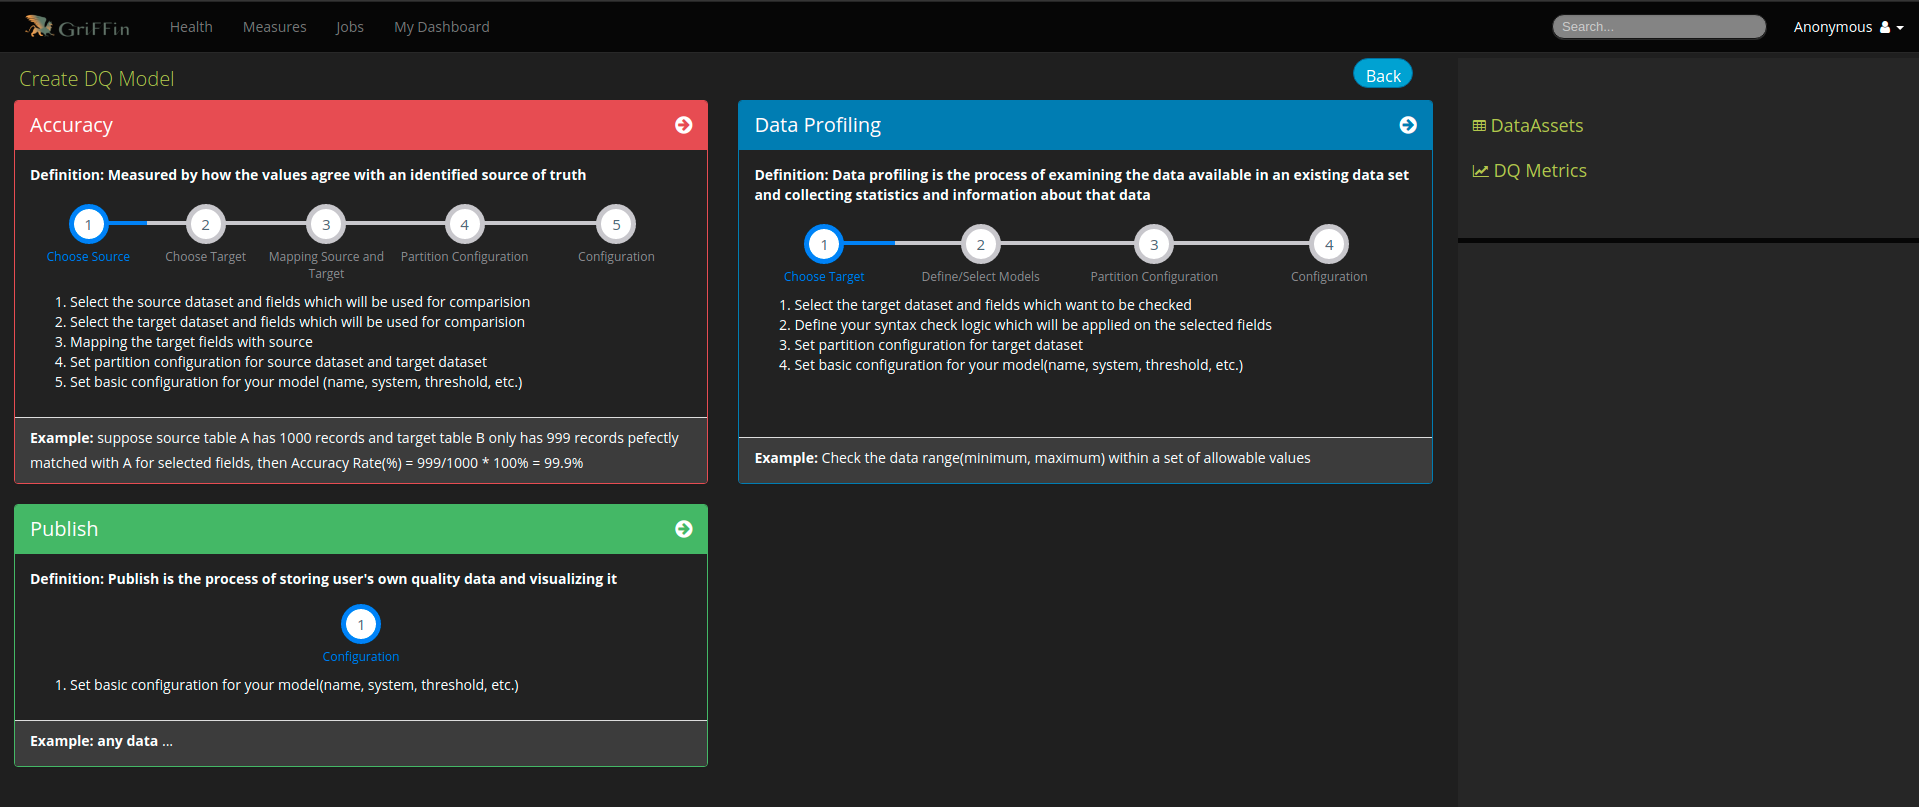
\includegraphics[scale=0.25]{Main/Static/UI_griffin.png} 
     \end{center}
\end{figure}
Le module Service, repr\'esente donc le web service de Apache Griffin. Développé en Java avec le \textit{framework} Spring Boot, il expose une \acrshort{api} \acrshort{rest}ful tr\`es riche. Elle offre bien plus de possibilit\'es qu'une utilisation via l'interface graphique, mais dans ce cas n\'ecessite de faire recours \`a un client tel que Postman pour les tests. Le calcul des diff\'erentes m\'etriques est fait par le module Measure, qui quant \`a lui est \'ecrit en Scala. 
\\
\begin{figure}[H]
    \caption{Interroger Apache Griffin avec Postman} \label{fig:xray}
    \begin{center}
      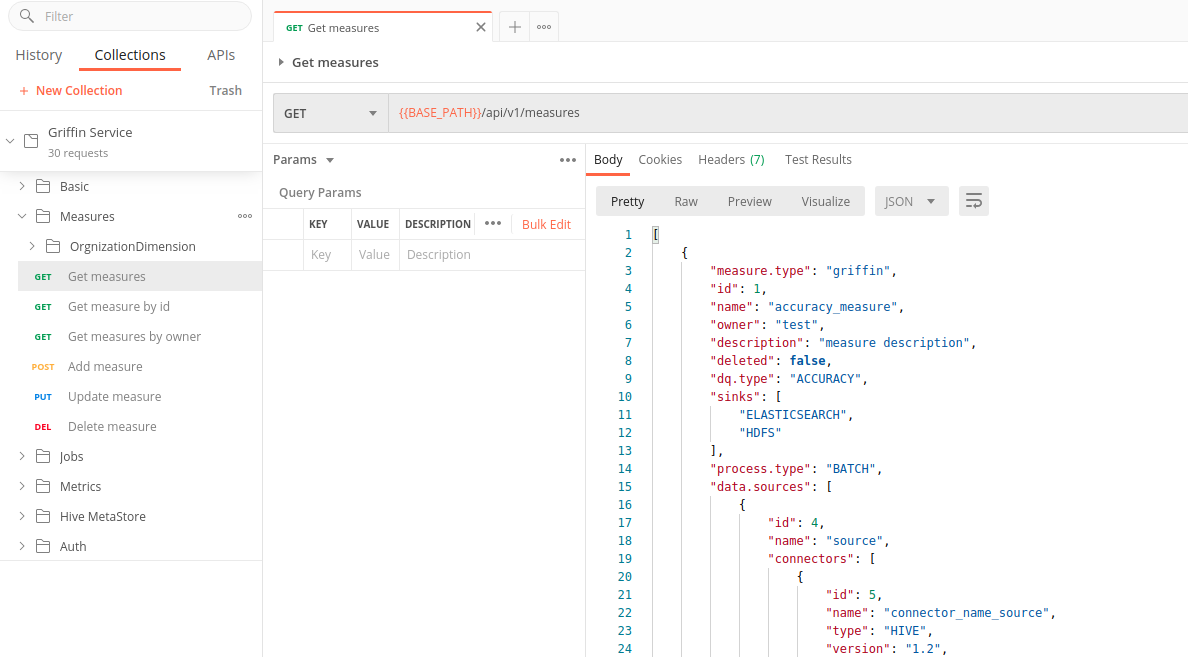
\includegraphics[scale=0.35]{Main/Static/Postman_Griffin.png} 
     \end{center}

\end{figure}
 
%\newpage
\subsubsection{\textbf{Couches de fonctionnement de Apache Griffin}}

Une vue m\'eso de l'architecture de Apache Griffin met en \'evidence trois (3) principales couches: Analyze, Measure et Define chacune jouant un r\^ole fondamental dans le fonctionnement de Griffin. D'abord, nous avons la couche Define, qui est responsable de la d\'efinition des dimensions de qualit\'e. Ensuite, vient la couche Measure qui permet le calcul des diff\'erentes m\'etriques. Les r\'esultats sont stock\'es dans le r\'ef\'erentiel de la derni\`ere couche : Analyze. Elle s'occupe de la sauvegarde et de l'affichage des r\'esultats. 

\begin{figure}[!h]
    \caption{S\'equences de fonctionnement de Apache Griffin}  \label{fig:xray}
    \begin{center}
      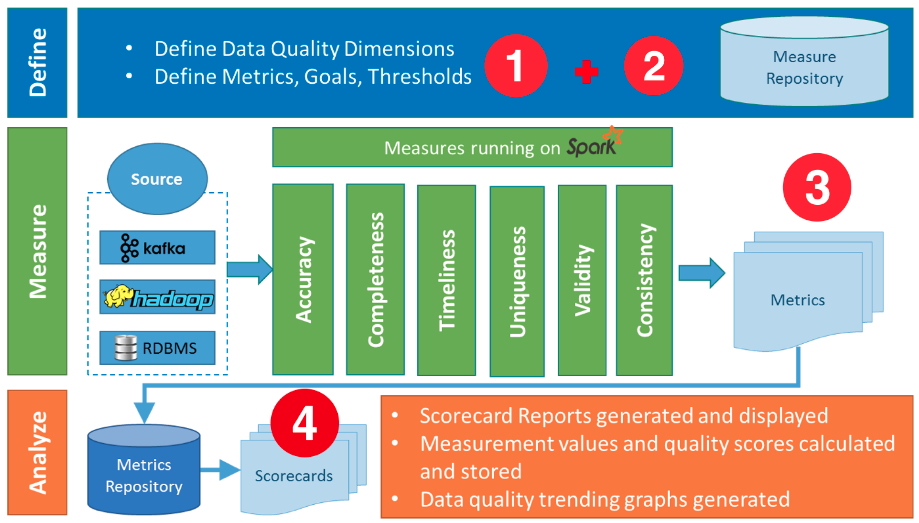
\includegraphics[scale=0.5]{Main/Static/Sequences_de_fonctionnement_Griffin.png} 
    \end{center}
\end{figure}
Suivant cette architecture, on a un flux de travail se pr\'esentant comme suit :

\begin{enumerate}[parsep=0cm,itemsep=0cm]
\item Enregistrement de la source ou des sources de données ;
\item Configuration des r\`egles de qualit\'e, qui peuvent être définies à partir des dimensions de qualité de données ;
\item Planification  de la tâche à soumettre p\'eriodiquement au \textit{cluster} Spark et stockages des m\'etriques;
\item Visualisation des indicateurs sur l'interface et analyser le rendu : la carte thermique et le tableau de bord peuvent \^etre utilis\'es \`a cet effet.

\end{enumerate}
\vspace{0.2cm} 

\subsubsection{\textbf{Infrastructures de l'écosystème d'Apache Griffin}}
Au niveau micro, Apache Griffin est un outil qui d\'epend et utilise plusieurs autres infrastructures \textit{big data} pour l'ex\'ecution des t\^aches. Nul besoin de pr\'eciser qu'on ne saurait parler d'infrastructures \textit{big data} sans citer Apache Hadoop et Apache Spark en premier lieu. Ainsi on y trouve les applications suivantes :

\begin{itemize}[parsep=0cm,itemsep=0cm]
\item \textbf{Apache Hadoop} (version 2.6.0 ou plus) : c'est un \textit{framework} de stockage et de traitement distribu\'e de grands ensembles de donn\'ees sur des \textit{clusters} d'ordinateur. Il sert de source de donn\'ees et au stockage des m\'etriques pour les traitements \textit{batch}. Toute l'architecture repose sur Hadoop;

\item \textbf{Apache Spark }(version 2.2.1 ou plus ): c'est un moteur de calcul distribu\'e et de traitement rapide des donn\'ees, d\'edi\'e au \textit{big data}. Le calcul des m\'etriques est effectu\'e sur Spark pour un gain maximal de performance ;

\item \textbf{Apache Hive} (version 2.x ): il s'agit d'un entrep\^ot de donn\'ees qui sert de \textit{metastore} et \'egalement de source de donn\'ees pour Griffin;

\item \textbf{PostgreSQL} (version 10.4 ou plus) ou \textbf{MySQL} (version 8.0.11 ou plus) :  ce sont des Syst\`emes de Gestion de Bases de Donn\'ees Relationnelles qui servent ici au stockage des diff\'erentes configurations en termes de dimensions de qualit\'e  et ainsi que les d\'etails concernant l'ex\'ecution (model store, asset store, job store) ;

\item \textbf{Livy} : permet de soumettre de façon programmatique des jobs spark  depuis des applications web/mobiles. Il s'agit d'une \acrshort{api} \acrshort{rest}ful ;

\item \textbf{Elasticsearch} (version 5.0 ou plus ): quant \`a lui permet \'egalement de stocker les r\'esultats (m\'etriques) issus de l'analyse de la qualit\'e des donn\'ees;

\item \textbf{Kafka} : Kafka est utilisé principalement pour la mise en place de flux de donn\'ees en temps réel.

\end{itemize}
%\vspace{0.15cm}
Griffin int\`egre \'egalement les d\'ependances suivantes : 

\begin{itemize}[parsep=0cm,itemsep=0cm]
\item \textbf{JDK} pour \acrlong{jdk};
\item \textbf{Scala};
\item \textbf{Maven} qui est un outil de  gestion de projet, utilisé pour empaqueter le projet Apache Griffin en fichier \textit{.jar};
\end{itemize}
\section{Installing and connecting Griffin to PostgreSQL}
\subsubsection{Tool installation}
To install Apache Griffin and make the configurations, we used the following architecture:
\begin{figure}[H]
    \caption{Architecture implemented to test Apache Griffin}  \label{fig:xray}
    \begin{center}
      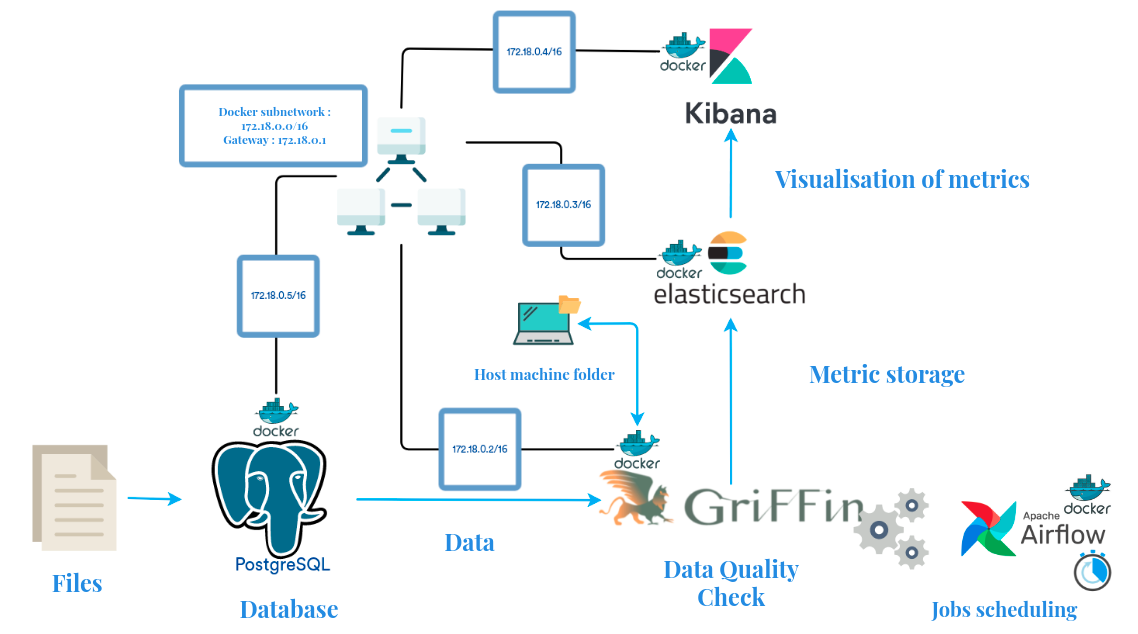
\includegraphics[scale=0.40]{Main/Static/Arch_eng.png} 
    \end{center}
\end{figure}
The installation is done via docker and takes place in two main steps, according to the documentation \cite{ApacheGriffinDocDocker}. First, a preparation of the working environment is required. This step is carried out in three (3) essential points:
\begin{enumerate}[parsep=0cm,itemsep=0cm]
    \item the installation of docker and docker compose;
    \item increasing the virtual memory limits for the use of Elasticsearch;
    \item retrieving the docker images needed for the installation. 
\end{enumerate}
After preparing the environment, the next step is the creation of the different docker containers.

\subsubsection{Connection to PostgreSQL}
Assessing the quality of data obviously requires data. For this purpose, Griffin allows you to configure access to different data sources. In particular, in batch mode, Griffin can audit the quality of data located in Hive tables, AVRO files, flat files (Parquet, \acrfull{csv}, \acrfull{tsv}, \acrfull{orc}) and data from sources with \acrshort{jdbc} (\acrlong{jdbc}) drivers such as Oracle, MySQL, PostgreSQL, etc. However, the connection to a PostgreSQL database was not natively supported.  To remedy this, we have modified the source code of the application. This modification involves adding the PostgreSQL database connection driver to the project dependencies. Then at the level of the test files, it was necessary to adapt the code, so that at the phase of build of the project, the driver once downloaded is suitably added to the Classpath. 

\section{Evaluation of the quality of the Digital Factory's data}
The second phase of the project aims to evaluate the quality of some tables with Griffin and to propose corrective measures where possible. For this purpose, two data extractions were provided. These are the 'Detail\_Victimes' and 'Inventaire\_Sinistre' tables. The 'Detail\_Victimes' table contains the information of all deceased or injured victims of an insurance claim as well as the differents assessments history. The 'Inventaire\_Sinistre' table contains the entire claim inventory, including settlements, reserves, and recoveries. The results of the evaluation are presented along each dimension.

\subsubsection{Uniqueness dimension}
For this dimension, we also highlighted for each targeted column three (3) metrics: the total number of observations in the column, the number of distinct observations and the number of distinct observations appearing more than once. The results of this assessment revealed that there were repetitions in the different columns. However, this did not constitute anomalies. This is due to the fact that the data is derived from the join between several tables.

\subsubsection{Validity dimension}
In this dimension we evaluated three (3) main rules. The objective was to identify the range of variation of the quantitative columns, to define the modalities of the different qualitative columns and to highlight the values presenting problems of encoding of accentuated characters. As a result of the evaluation,  we have highlighted encoding problems in the \textit{'Beneficiaire'} column of the 'Detail\_Victimes' table. The encoding problems as we detected them are characterised by the appearance of '?' in place of accented characters. Thus 'p\`ere' is spelled out as 'p?re' for example.

\subsubsection{Completeness dimension}
We use three (3) metrics to assess this dimension: the total number of rows, the number of incomplete observations and the number of non-zero observations. We have eighty (80) columns with missing values for 'Detail\_Victimes'  i.e. about 86\% of the table's columns, and 39 columns for 'Inventaire\_Sinistre', i.e. about 43\% of the columns.

\begin{figure}[H]
    \caption{Completeness 'Detail\_Victimes'}  \label{fig:xray}
    \begin{center}
      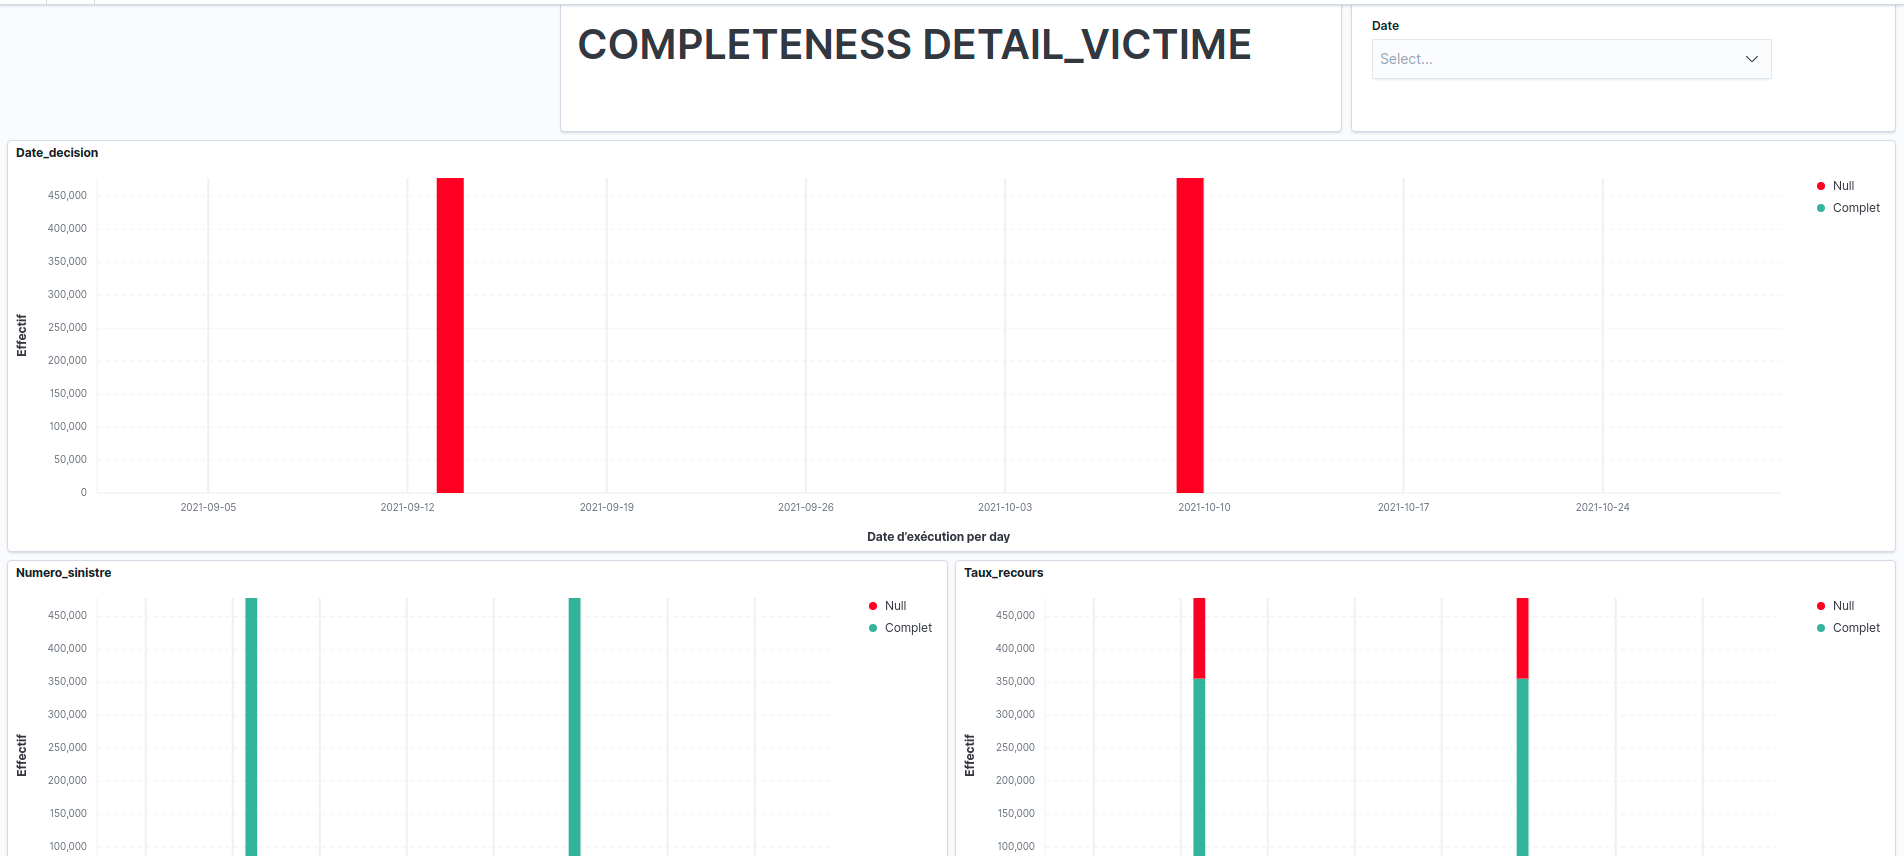
\includegraphics[scale=0.27]{Main/Static/Completeness_Detail_Victime.png} 
    \end{center}
\end{figure}



\subsubsection{Consistency Dimension}
\textbf{'Inventaire\_Sinistre' table}\\
The rules established at the level of this dimension, allow to attest the consistency of the data with the business rules. It is expected that the formulas for the calculation of the charge, the total settlement and the total provision are respected. We also checked the consistency of the dates. Logically, the date of occurrence of the claim, the date of opening of the file and the date of birth of the driver should be earlier than the date of declaration of the claim, the date of closure and the date of licence respectively. In addition to these rules, we have assessed the consistency of the nature of the claim, whether it is 'Bodily' or 'Material'. Indeed, a claim that results in injury and/or loss of life cannot be classified as 'Material'. On the other hand, some claims may be classified as 'Bodily' if they cost more than 100,000 Moroccan dirham even though there are no injuries or deaths. These different rules make it possible to assess the consistency of the nature of the claim. We discovered : 
\begin{itemize}[parsep=0cm,itemsep=0cm] 
    \item 1 claim of a 'Material' nature but with 5 injured victims and 1 deceased;
    \item 237,657 claims with a cost of less than 100,000 Moroccan dirham, with no victims recorded but of a 'Bodily' nature;
    \item 190,622 claims where the number of victims is unequal to the count in the 'Detail\_Victimes' table;
    \item 102 observations for which the claim is declared before it occurs;
    \item 3,972 observations for which the date of obtaining a driving licence is earlier than the date of birth;
    \item 76,000 observations with file opening dates chronologically later than the file closing date.
\end{itemize}
\textbf{'Detail\_Victimes' table}\\
We verify whether the amounts of medical and pharmaceutical expenses and those of permanent partial disability are correctly entered, in accordance with the amount indicator variables. A check has also been made on the consistency of the date of occurrence and declaration. The execution of the rules revealed the following results: 19,082 observations are affected by an inconsistency between the dates of occurrence and declaration. Moreover, when the indicator variable takes the value 'N', meaning that there should be no expenses (medical and pharmaceutical or permanent partial disability), there is sometimes an amount present.

\section{Correction and quality improvement}
The review of the state of data quality identified columns with various anomalies. However, not all of these anomalies constitute errors. Once the selection had been made, we undertook to apply corrections to the columns with consistency problems, as well as a correction of the encoding problems. The various corrections were applied using PySpark (version 2.4.7). This is a Python interface for Apache Spark. 

\subsubsection{Reliability of the number of victims and the nature of the disaster}
In order to correct the differences in the number of injured and deceased victims in the 'Inventaire\_Sinistre' table, the number of injured and deceased victims was counted for each loss in the 'Detail\_Victimes' table. This new data, together with the information contained in the 'Inventaire\_Sinistre' table, produced a new column giving the number of injured and dead for each claim with a corresponding value in the 'Detail\_Victimes' table. With these new values, we proceeded to adjust the nature of the incident. If the number of injured or dead is greater than zero (0), then the claim type is 'Bodily'. Otherwise, if the charge is less than or equal to 100,000 Moroccan dirham and the claim was previously classified as 'Bodily', it is reclassified as 'Material'. Indeed, there is no reason to consider it as a 'Bodily' claim. On the other hand, if none of the above conditions are met and the charge is strictly greater than 100,000 Moroccan dirham or a claim of a 'Material' nature, then the value of the initial variable \textit{'Nature\_Sinistre'} is retained. This adjustment algorithm leads to the creation of a new variable \textit{'Nature\_Sinistre\_New'}.

\subsubsection{Algorithm for correcting encoding problems}
The targets of our correction are the words of the dictionary (not the proper names). The algorithm algorithm used uses Levenshtein's distance to identify the most likely spelling corrections for a word : these are the candidate words. Levenshtein's distance is a measure of similarity between two strings. It is equal to the number of elementary operations to do to transform a string M into a string P. These are :
\begin{itemize}[parsep=0cm,itemsep=0cm]
    \item substitution of a character ;
    \item insertion or addition of a character ;
    \item deleting or erasing a character.
\end{itemize}

Once the list of candidate words has been obtained, the algorithm then compares all the candidates with a dictionary of words. The particularity of this dictionary is that it associates each word with a frequency of occurrence. The key is the word and the value is the frequency of the word. The candidate with the highest frequency of occurrence is more likely to be the correct result. In case of co-occurrence an alphabetical ranking is performed. This algorithm is implemented in Python by the SpellChecker library. 

\subsubsection{Reliability of indicator variables}
Any amount strictly greater than zero (0) must be materialized by the modality 'Y' in the indicator variable. The correction of these inconsistencies is therefore done using the following algorithm: if the amount is greater than zero (0), a new indicator variable is assigned the value 'Y'. Otherwise, the value 'N' is returned to indicate that there is no charge. The correction results in the creation of a new column so that the existing data is not altered. The algorithm implemented allowed the correction of inconsistencies and the imputation of missing values of indicator variables.
%\section{Limites et perspectives d'Apache Griffin}

La documentation d'Apache Griffin fournit une feuille de route sur les prochaines fonctionnalit\'es \`a d\'evelopper ainsi que celles disponibles. N\'eanmoins, certaines fonctionnalit\'es actuellement disponibles, pr\'esentent les limites suivantes: 
\begin{description}[parsep=0cm,itemsep=0cm]
\item[la gestion des mesures] : En effectuant des op\'erations sur l'interface utilisateur, on ne peut que cr\'eer, supprimer et mettre \`a jour que trois types de mesures. Les appels par l'\acrshort{api}, offrent \`a l'utilisateur un panel plus vari\'e de mesures (accuracy, profiling, timeliness, uniqueness ou distinctness, completeness, publish metrics). Toutefois l'absence d'impl\'ementation de connecteur de type \acrshort{jdbc} au niveau du web service limites assez la vari\'et\'e des sources;

\item[la gestion de l'ex\'ecution des mesures (jobs)]: L'utilisateur ne peut créer, modifier, supprimer et  planifier des jobs pour les donn\'ees venant par \textit{batch}, uniquement que pour les mesures \'elabor\'ees pour les connexions de type HIVE, AVRO, CUSTOM, via Postman. 
\end{description}
De plus, la mesure de type Uniqueness pr\'esente quelques dysfonctionnements et la Publish Metrics n'est pas document\'ee, faute de quoi nous n'avons pas pu la tester. Pour cette derni\`ere nous soupçonnons une obsolescence de la fonctionnalit\'e. Car m\^eme dans le code source elle s'est av\'er\'ee absente. Notons \'egalement que la documentation sur github bien que d\'etaill\'ee, n'est pas tenue \`a jour. 
\\

\`A court-terme, Apache Griffin envisage de supporter plus de sources de donn\'ees. Notamment un enrichissement de la connexion aux bases de donn\'ees relationnelles, ainsi qu'une connexion \`a Elasticsearch. De plus, Griffin pr\'evoit prendre en charge de mani\`ere native d'autres dimensions de qualit\'e de donn\'ees comme la coh\'erence et la validit\'e. Pour l'instant, il est laiss\'e \`a la charge de l'utilisateur la d\'efinition des attentes vis-\`a-vis de ces dimensions. Une nouvelle fonctionnalit\'e est \'egalement cibl\'ee:  il s'agit de la d\'etection d'anomalie en analysant les m\'etriques calcul\'ees par Elasticsearch. Notons \'egalement que dans le cadre de cette \'etude, nous avons utilis\'e la version 0.6.0 d'Apache Griffin, mais durant cette exploration, de nouvelles fonctionnalités et des am\'eliorations de celles existantes ont \'et\'e publi\'ees sur github. Il s'agit de la réécriture et de la red\'efinition des diff\'erentes dimensions. Ainsi la nouvelle version s'appuiera probablement sur les dimensions suivantes :  l'Accuracy, la Completeness, la Duplication et le Profiling. En plus, de ces quatre dimensions Griffin intègre une nouvelle: la conformit\'e du sch\'ema. Cette mesure \'evalue si oui ou non les donn\'ees respectent le type qu'on leur attribue. Il est question l\`a de l'\'evaluation de la validit\'e des donn\'ees.  Ces modifications dans les mesures se traduisent aussi par une réécriture de la configuration du fichier \textit{.json} ainsi que de la pr\'esentation des r\'esultats. En termes de connectivit\'e, une classe pour la connexion \`a Elasticsearch a \'egalement \'et\'e ajout\'ee. Ce qui annonce de belles perspectives pour le d\'eveloppement de l'outil. 
\\



%Chapitre4
\chapter{ \'Evaluation et am\'elioration de la qualit\'e des donn\'ees de la Digital Factory }
\section*{Introduction}
Le choix d'un outil d\'edi\'e \`a la qualit\'e des donn\'ees, est une \'etape essentielle dans le processus de gestion et d'industrialisation de la qualit\'e. Une fois l'installation et les configurations faites, on peut ais\'ement proc\'eder \`a l'\'evaluation de la qualit\'e ainsi qu'\`a la fiabilisation des donn\'ees. Ce chapitre pr\'esente les r\'esultats issues de l'\'evaluation de la qualit\'e des tables 'Detail\_Victimes' et 'Inventaire\_Sinistre', de m\^eme que les algorithmes de correction mis en place.

\section{D\'efinition de quelques concepts m\'etiers}
\subsubsection{\textbf{Sinistre}}
Un sinistre est la réalisation de l'événement couvert par le contrat et qui donne lieu aux prestations assurées : indemnité, capital ou rente, assistance…
\subsubsection{\textbf{Charge d'un sinistre}}
 On d\'efinit la \textbf{charge} d'un sinistre, comme \'etant le co\^ut total du sinistre. Elle repr\'esente le montant que l'assureur doit payer \`a l'assur\'e. 
 
 \subsubsection{\textbf{Provision d'un sinistre}}
 La \textbf{provision} quant \`a elle, est l'ensemble des montants accumul\'es par l'entreprise d'assurances et de r\'eassurance pour faire face \`a ses engagements envers les assur\'es et b\'en\'eficiaires de contrats d'assurance. 
 
 \subsubsection{\textbf{R\`eglement du sinistre}}
 Le \textbf{r\`eglement} d'un sinistre d\'esigne le montant vers\'e comme indemnit\'e par l'assureur \`a l'assur\'e. 
 
 \subsubsection{\textbf{Recours}}
 Le \textbf{recours} quant à lui est une action amiable (lettres, mise en demeures) ou judiciaire (assignation), entreprise par la victime et/ou l'assureur contre le(s) responsable(s) du pr\'ejudice subi et/ou assureur dans le but d'\^etre d\'edommag\'e. On parle de recours \'emis, lorsqu'on se positionne du c\^ot\'e de la partie émettrice du recours. On parlera de recours subis lorsqu'on se place du c\^ot\'e de la partie qui reçoit le recours. 
 
 \subsubsection{\textbf{B\'en\'eficiaire}}
 Le b\'en\'eficiaire est une tierce personne physique ou morale, au profit de laquelle l'assurance a été contractée. Elle peut être nommément désignée aux conditions particulières du contrat ou bien apparaître dans les conditions générales sous les termes de : conjoint, p\`ere, m\`ere, ...
 
 
\section{Évaluation de la qualité de la donnée de la \acrlong{df}}
La premi\`ere phase de notre projet consistait \`a prendre en main Apache Griffin, afin de le configurer pour qu'il puisse r\'epondre aux besoins de la \acrshort{df}. Une fois achev\'ee,  la deuxi\`eme phase du projet a pour but d'\'evaluer \`a l'aide de l'outil, la qualit\'e des donn\'ees du socle, et de proposer des mesures de redressement lorsque cela est possible. \`A cet effet, deux extractions de donn\'ees ont \'et\'e fournies. Il s'agit des tables 'Detail\_Victimes' et 'Inventaire\_Sinistre'. La table 'Detail\_Victimes' contient les informations de toutes les victimes décédées ou blessées ainsi que l'historique des évaluations. La table 'Inventaire\_Sinistre' quant \`a elle contient tout l'inventaire du sinistre, y compris les règlements, les provisions, et les recours. Elles ont \'et\'e import\'ees dans PostgreSQL, suite \`a la cr\'eation d'une base de donn\'ees et la d\'efinition du sch\'ema des diff\'erentes tables. 


Au cours de l'importation, des anomalies ont \'et\'e d\'etect\'ees dont notamment la pr\'esence de chaîne de caract\`eres vide dans les colonnes '\emph{Resp}' des deux (2) tables. Ces colonnes sont cens\'ees contenir des donn\'ees num\'eriques. De plus, le format (JJ/MM/AAAA) de toutes les colonnes contenant des donn\'ees de type \textit{date} dans la table 'Inventaire\_Sinistre', \'etait incompatible avec le format attendu par PostgreSQL (AAAA-MM-JJ). Afin de contourner ces diff\'erentes difficult\'es, nous avons import\'e les colonnes '\emph{Resp}' au format \textit{varchar(100)}, remplac\'e les chaînes de caract\`eres vide par \textit{null} puis proc\'ed\'e \`a un transtypage au format \textit{real}. De m\^eme, pour les colonnes contenant des dates, nous avons proc\'ed\'e \`a une importation au format \textit{varchar(100)} puis un transtypage au format \textit{date},le tout automatis\'e dans un script \acrshort{sql}. Une fois nos donn\'ees import\'ees dans PostgreSQL, nous avons r\'ealis\'e l'\'evaluation de la qualit\'e  de chaque table avec Griffin. Les r\'esultats sont pr\'esent\'es suivants chaque dimensions.

\subsection{Pr\'esentation des donn\'ees}
\begin{table}[H]
\caption{Composition des diff\'erentes tables}
{\footnotesize
\begin{center}
\begin{tabular}{llcc}
\toprule 
&& \textbf{Detail\_Victimes} & \textbf{Inventaire\_Sinistre} \\
\midrule
\textbf{Nombre de lignes} && 477 942 & 1 885 568 \\ 
\textbf{Nombre de colonnes} && 93 & 90 \\
\textbf{Attributs de type chaîne de caract\`eres} && 26 & 48 \\
\textbf{Attributs de type r\'eel} && 57 & 25 \\
\textbf{Attributs de type entier} && 2 & 6 \\
\textbf{Attributs de type date} && 8 & 11 \\
\bottomrule
\end{tabular}
\end{center}}
\end{table}

Nous allons \'egalement pr\'esent\'e quelques variables qui interviendront dans la suite.

%\begin{table}[h]
\topcaption{Quelques variables de la table 'Inventaire\_Sinistre'}
%\vspace{0.5cm}
{\footnotesize
\begin{center}
\begin{supertabular}{lcl}
\toprule 
& \textbf{Inventaire\_Sinistre} &  \\
\midrule
\textbf{Variable}                                 & \textbf{Type}                         & \textbf{Description}  \\
\hline 
\textbf{NUMERO\_SINISTRE}                          & Cha\^ine de caract\`eres    & Identifiant du sinistre   \\ 
DATE\_SURVENANCE                          & Date                        & Date survenance du sinistre   \\ 
DATE\_DECLARATION                         & Date                        & Date Déclaration du sinistre   \\ 
DATE\_OUVERTURE                           & Date                        & Date Ouverture du dossier sinistre   \\ 
DATE\_CLOTURE                             & Date                        & Date Clôture du dossier sinistre\\ 
DATE\_NAISSANCE\_CONDUCTEUR               & Date                        & Date de naissance du conducteur   \\ 
DATE\_PERMIS                              & Date                        & Date du permis\\ 
CHARGE                                    & R\'eel                      & Coût total du sinistre   \\ 
PROVISION\_TOTAL                          & R\'eel                      & Provision du sinistre   \\ 
REGLEMENTS\_TOTAL                         & R\'eel                      & Reglements du sinistre   \\ 
VICTIMES\_BLESSEES                        & Entier                     & Nombre de victimes blessées dans le sinistre \\
VICTIMES\_DECEDEES                        & Entier                     & Nombre de victimes décédées dans le sinistre\\
NATURE\_SINISTRE                          & Cha\^ine de caract\`eres    & Nature du sinistre (corporel ou materiel) \\
\bottomrule
\end{supertabular}
\end{center}}

%\end{table}

\begin{table}[H]
\caption{Quelques variables de la table 'Detail\_Victime'}
%\vspace{0.5cm}
{\footnotesize 
\begin{center}
\begin{tabular}{lcl}
\toprule 
& \textbf{Detail\_Victimes} &  \\
\midrule
\textbf{Variable}                                 & \textbf{Type}                         & \textbf{Description}  \\
\hline 
NUMERO\_SINISTRE                          & Cha\^ine de caract\`eres    & Identifiant du sinistre   \\ 
DATE\_SURVENANCE                          & Date                        & Date survenance du sinistre   \\ 
DATE\_DECLARATION                         & Date                        & Date Déclaration du sinistre   \\ 
BENEFICIAIRE                             & Cha\^ine de caract\`eres     & Désigne le b\'en\'eficiaire   \\ 
FRAISMEDPHARMA                           & R\'eel                       & \acrfull{fmp} \\
RSK\_FMPVALINIT\_IND                     & Cha\^ine de caract\`eres     & Indicateur \acrshort{fmp}(Y/N)\\
MONTANT\_IPP                             & R\'eel                       & Montant \acrfull{ipp}\\
RSK\_IPPVALINIT\_IND                     & Cha\^ine de caract\`eres     & Indicateur \acrshort{ipp}(Y/N)        \\
NATUREDESDEGATS                          & Cha\^ine de caract\`eres     & Nature des d\'egats(Bless\'e,Mortel) \\
NATURE\_SINISTRE                          & Cha\^ine de caract\`eres     & Nature du sinistre (corporel ou materiel) \\
VICTIMEKEY                               & Cha\^ine de caract\`eres     & Identifiant de la victime \\
\bottomrule
\end{tabular}
\end{center}}

\end{table}


\normalfont
\subsection{Dimension de Compl\'etude} 
Nous utilisons ici trois (3) m\'etriques pour appr\'ecier cette dimension: le nombre total de lignes, le nombre d'observations incompl\`etes et le nombre d'observations non nulles. Elles sont calcul\'ees comme suit: 
\begin{lstlisting}[language=SQL,caption={R\`egles de la Dimension Compl\'etude},captionpos=t ,showspaces=false,basicstyle=\scriptsize,numbers=none,commentstyle=\color{gray},backgroundcolor=\color{background}]
--total : 
SELECT COUNT(*) AS total FROM source, save as table total_count

--nombre d'enregistrements incomplets: 
SELECT COUNT(*) as incomplete FROM source 
WHERE NOT (numero_contrat IS NOT NULL), save as table incomplete_count

--nombre d'enregistrement complets: 
SELECT (total_count.total - incomplete_count.incomplete) AS complete 
FROM source LEFT JOIN incomplete_count, save as table complete_count
\end{lstlisting}
Cette dimension est ex\'ecut\'ee pour toutes les colonnes des deux tables. Nous avons obtenu les r\'esultats suivants:  
\begin{itemize}[parsep=0cm,itemsep=0cm]
\item table 'Detail\_Victimes': quatre-vingt (80) colonnes ont des valeurs manquantes (soit environ 86\%) dont cinq (5) compl\`etement vides, dix (10) ayant \`a peine 10\% de valeurs compl\`etes et vingt (20) avec un taux de valeurs manquantes compris en 20 et 50\%;
\item table 'Inventaire\_Sinistre': on compte trente-neuf (39) colonnes avec des valeurs manquantes (soit environ 43\%) dont cinq (5) enti\`erement nulles et six (6) avec plus de 30\% de valeurs nulles.
\end{itemize}
Voici un aperçu du tableau de bord:
\begin{figure}[H]
        \caption{Visualisation de la dimension Compl\'etude pour la table 'Detail\_Victimes'}  \label{fig:tttay}
    %\advance\rightskip-2cm
    %\advance\leftskip-4cm
    \begin{center}
      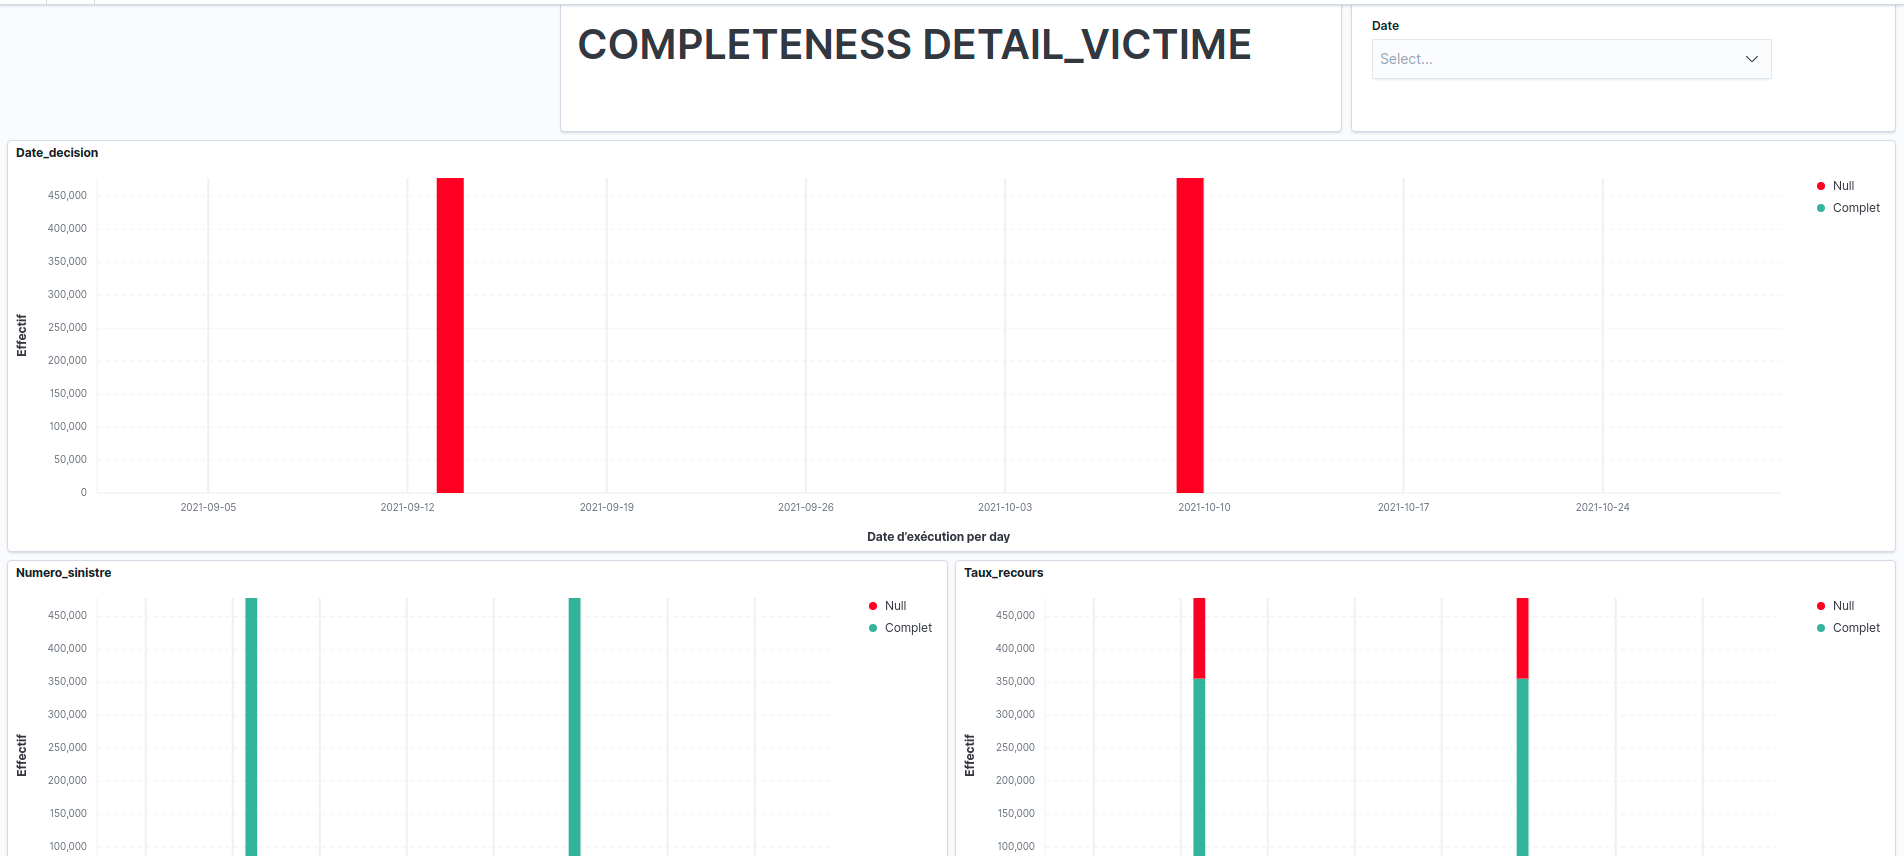
\includegraphics[scale = 0.27]{Main/Static/Completeness_Detail_Victime.png} 
    \end{center}
\end{figure}
Toutefois, toutes les colonnes pr\'esentant des valeurs manquantes n'ont pas pour autant des probl\`emes de qualit\'e. Il peut s'agir d'une r\'eponse inappropri\'ee au regard du contexte. Afin de pousser plus loin l'\'evaluation de la qualit\'e, une analyse de la p\'eriode couverte par ces valeurs manquantes fut faite au niveau de la dimension de coh\'erence.

\subsection{Dimension d'Unicit\'e}
Pour cette dimension, nous avons \'egalement fait ressortir pour chaque colonne cibl\'ee trois (3) m\'etriques :  le nombre total d'observations dans la colonne, le nombre d'observations distinctes et le nombre d'observations distinctes apparaissant plus d'une fois. Les r\`egles ayant permis d'obtenir ces m\'etriques sont les suivantes : 
\newpage
\begin{lstlisting}[language=SQL,caption={R\`egles de la Dimension Unicit\'e},captionpos=t,showspaces=false,basicstyle=\scriptsize,numbers=none,commentstyle=\color{gray},backgroundcolor=\color{background}]
--total_numero_contrat et distinct_numero_contrat: 
SELECT COUNT(src.numero_contrat) AS total_numero_contrat, 
COUNT(DISTINCT src.numero_contrat) as distinct_numero_contrat FROM src 

--duplicated_numero_contrat: 
SELECT COUNT(tmp.numero_contrat) as duplicated_numero_contrat 
FROM (SELECT numero_contrat FROM src GROUP BY numero_contrat 
HAVING COUNT(numero_contrat) > 1) as tmp
\end{lstlisting}

\begin{figure}[H]
        \caption{Visualisation de la dimension Unicit\'e pour la table 'Inventaire\_Sinistre'}  \label{fig:tttay}
    %\advance\rightskip-2cm
    %\advance\leftskip-4cm
    \begin{center}
      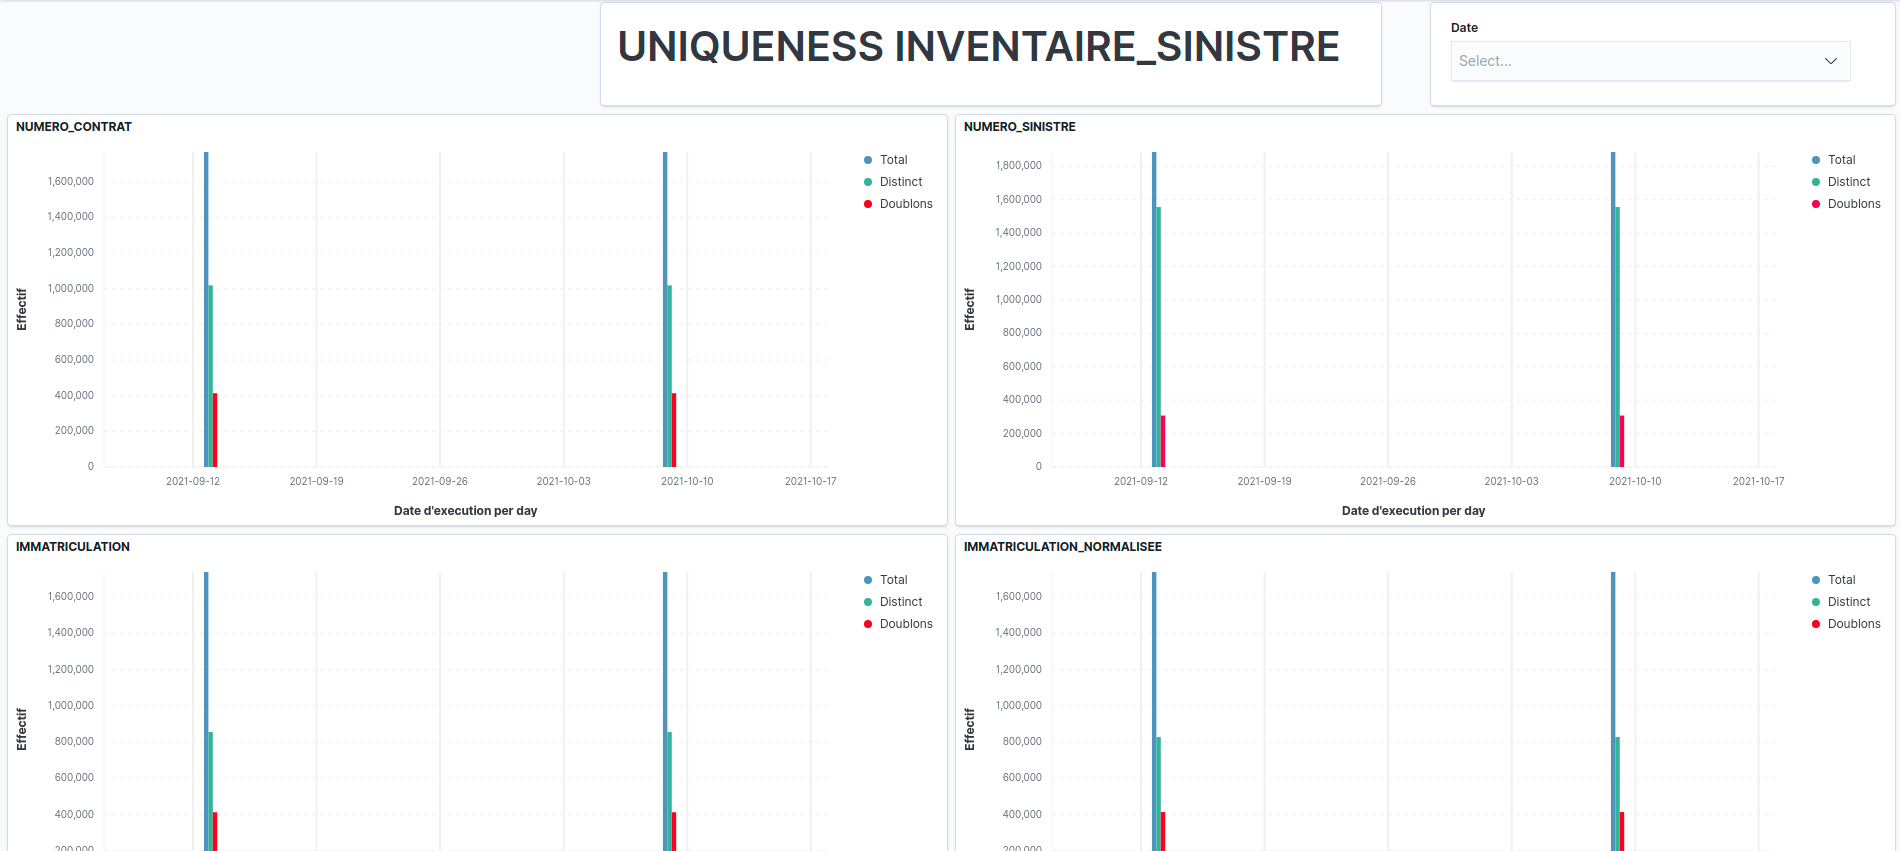
\includegraphics[scale = 0.27]{Main/Static/Uniqueness_Inventaire_Sinistre.png} 
    \end{center}
\end{figure}
Ces r\`egles sont appliqu\'ees, sur des colonnes pr\'esentant \`a priori des contraintes d'unicit\'e ou repr\'esentant des num\'eros ou codes d'identification. Les r\'esultats issus de cette \'evaluation ont r\'ev\'el\'e qu'il y avait des r\'ep\'etitions au niveau des diff\'erentes colonnes. Mais cela ne constituait pas n\'eanmoins des anomalies. Cela s'explique par le fait que les donn\'ees sont issues de la jointure entre plusieurs tables.


\subsection{Dimension de Validit\'e} 
Au niveau de cette dimension nous avons \'evalu\'e trois (3) grandes r\`egles. L'objectif \'etait d'identifier la plage de variation des colonnes quantitatives, de d\'efinir les modalit\'es des diff\'erentes colonnes qualitatives et de faire ressortir les valeurs pr\'esentant des probl\`emes d'encodages de caract\`eres accentu\'es. Essentiellement les r\`egles \'evalu\'ees sont les suivantes : 
\newpage
\begin{lstlisting}[language=SQL,caption={R\`egles de la Dimension Validit\'e},captionpos=t,showspaces=false,basicstyle=\scriptsize,numbers=none,commentstyle=\color{gray},backgroundcolor=\color{background}]
--plage de valeurs numeriques (griffin-dsl): 
min(montant_evaluation) as montant_evaluation_minimal,
max(montant_evaluation) as montant_evaluation_maximal, 
avg(montant_evaluation) as montant_evaluation_moyenne

--differentes modalites:
SELECT DISTINCT(classe_victime) AS classe_victime_distinct from src

--detection des problemes d'encodage:
SELECT DISTINCT(beneficiaiare) FROM src 
WHERE beneficiaiare rlike '[a-zA-Z]+[?]+[a-zA-Z]*'
\end{lstlisting}
Suite \`a l'\'evaluation de cette dimension, nous avons mis en \'evidence comme anomalie des probl\`emes d'encodages dans la colonne '\textit{Beneficiaire}' de la table 'Detail\_Victimes'.  Les probl\`emes d'encodages tels que nous les avons d\'etect\'es sont caract\'eris\'es par l'apparition de '?' en lieu et place des caract\`eres accentu\'es. Ainsi p\`ere se retrouve écorché en 'p?re' par exemple.
\begin{figure}[H]
        \caption{Visualisation de la dimension Validit\'e pour la table 'Detail\_Victimes'}  \label{fig:tttay}
    %\advance\rightskip-2cm
    %\advance\leftskip-4cm
    \begin{center}
      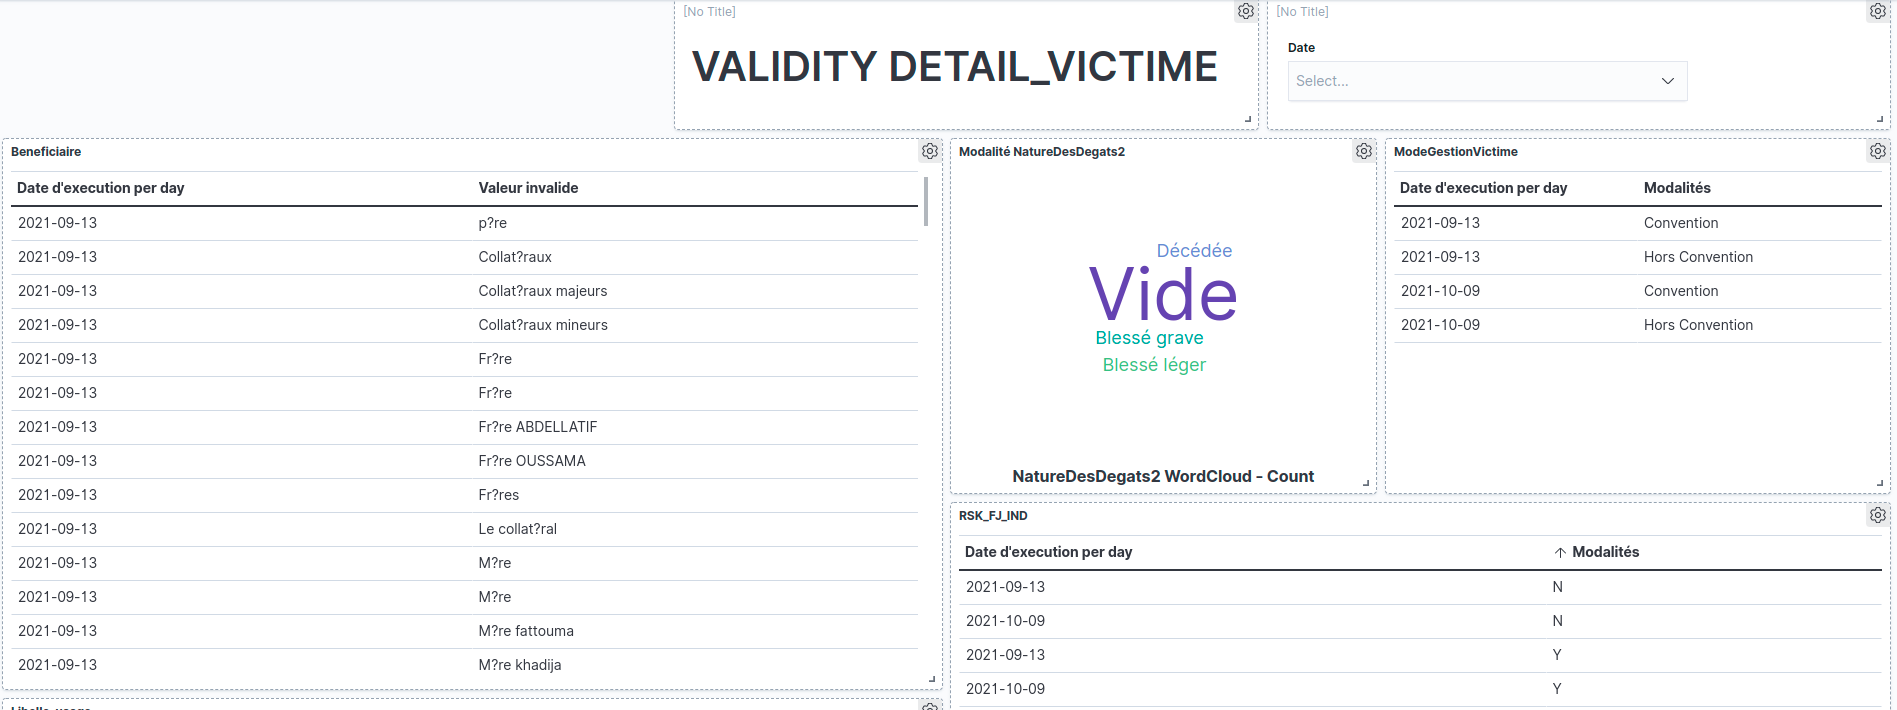
\includegraphics[scale = 0.27]{Main/Static/Validity_Detail_Victime.png} 
    \end{center}
\end{figure}

% De plus, bien que des valeurs n\'egatives aient \'et\'e d\'etect\'ees pour des variables repr\'esentant des montants, il s'est av\'er\'es que ces valeurs \'etaient utilis


\subsection{Dimension de Coh\'erence }
\subsubsection{\textbf{Table 'Inventaire\_Sinistre'}}
Les r\`egles \'etablies au niveau de cette dimension, permettent d'attester de la coh\'erence des donn\'ees vis-\`a-vis des r\`egles m\'etiers. La table 'Inventaire\_Sinistre' permet de capter les informations relatives \`a un sinistre, comme le co\^ut, le nombre de victimes, les dates cl\'es... On s'attend \`a ce que les formules actuarielles suivantes soient respect\'ees:
%\begin{equation}
%Charge = Provisions + Reglement - Recours\_encaissé - Recours\_a\_encaissé
%\end{equation}

\begin{equation}
  \begin{split}                                  
   Charge\_sinistre =  Reglement\_garantie + Reglement\_intervenant - \\
       Recours\_emis\_recuperer + Recours\_subis\_payer + \\
       Provisions\_garanties +  Provision\_intervenant - \\
        Provision\_recours\_emis + Provision\_recours\_subi -\\
        Recours\_emis + Recours\_subis
  \end{split}
\end{equation}

\begin{equation}
\begin{split}  
	Reglement\_total =  Reglement\_garantie + Reglement\_intervenant 
 \end{split}
\end{equation}

 
\begin{equation}
\begin{split}  
 Provisions\_total = Provisions\_garantie\_actuel + \\
 Provisions\_intervenant\_actuel  
\end{split}
\end{equation}
 Elles ont permis d'\'elaborer des r\`egles de qualit\'es. En effet, la coh\'erence au niveau de la charge repr\'esente une grosse probl\'ematique au sein de la \acrshort{df}. Nous avons \'egalement v\'erifi\'e la coh\'erence au niveau des dates. Logiquement, les date de survenance du sinistre, date d'ouverture du dossier et date de naissance du conducteur, doivent respectivement \^etre ant\'erieures aux date de d\'eclaration du sinistre, date de clôture et date de permis. Des incoh\'erences d\'etect\'ees \`a ce niveau, peuvent permettre de d\'eceler des cas de fraudes.\\

Par ailleurs, un sinistre peut \^etre qualifi\'e de Corporel, 'Materiel' ou 'Mixte' suivant la nature des d\'eg\^ats qu'il a provoqu\'e chez les victimes. Dans la table, seuls les sinistres de nature 'Corporel' et 'Materiel' sont pr\'esents. Ainsi, un sinistre ayant provoqu\'e des blessures et/ou caus\'e des pertes en vies humaines ne peut \^etre qualifi\'e de 'Materiel'. Ce qui est tout \`a fait logique. De m\^eme, certains sinistres peuvent \^etre affect\'es du qualificatif 'Corporel', s'ils ont co\^ut\'e plus de 100 000 dirham marocain bien qu'il n'y ait ni bless\'e ni mort. Ces diff\'erentes r\`egles permettent d'\'evaluer la coh\'erence des informations contenues dans les colonnes '\textit{Victimes\_Decedees}', '\textit{Victimes\_Blessees}' et '\textit{Nature\_Sinistre}'. Aussi, avec la table 'Detail\_Victime' qui contient les informations des diff\'erentes victimes d'un sinistre, on doit pouvoir retrouver le nombre total de victimes (bless\'ees ou d\'ec\'ed\'ees) de chaque sinistre dans l'inventaire. En plus de ces r\`egles, une attention particuli\`ere est port\'ee sur certaines colonnes afin d'identifier la p\'eriode couverte par les valeurs nulles. Un extrait des r\`egles se pr\'esente comme suit : 
\newpage
\begin{lstlisting}[language=SQL,caption={R\`egle de la Dimension Coh\'erence pour la table \textit{Inventaire\_Sinistre}},captionpos=t,showspaces=false,basicstyle=\scriptsize,numbers=none,commentstyle=\color{gray},backgroundcolor=\color{background}]
--regle de verification des formules: 
	--nombre d'enregistrements incoherents:
SELECT COUNT(*) FROM src WHERE 
power((reglements_total - reglement_garantie+reglement_intervenant),2)>1
	--echantillon incoherent
SELECT numero_sinistre, reglements_total, reglement_garantie,reglement_intervenant,
reglement_garantie+reglement_intervenant as somme_reglement 
FROM src 
WHERE power((reglements_total- reglement_garantie+reglement_intervenant),2)>1 
LIMIT 20

--regles de coherence des dates:
	--nombre d'enregistrements incoherents:
SELECT COUNT(*) AS nb_inconsitency_date_survenance_declaration FROM src 
WHERE date_survenance > date_declaration 
	--echantillon incoherent
SELECT numero_sinistre,date_survenance,date_declaration,statut_sinistre 
FROM src WHERE date_survenance > date_declaration LIMIT 20

--periode d'apparition des valeurs nulle:
SELECT MIN(date_creation_systeme), MAX(date_creation_systeme) FROM src 
WHERE COALESCE(numero_contrat,'empty') ='empty'

--regle de coherence nature_sinistre
SELECT COUNT(*) FROM  
(SELECT numero_sinistre FROM src WHERE nature_sinistre = 'Materiel' 
GROUP BY numero_sinistre HAVING SUM(victimes_blessees)> 0 
and SUM(victimes_decedees) >0)T

--regle de coherence nombre de victimes
SELECT COUNT(*) FROM 
(SELECT numero_sinistre, SUM(victimes_decedees) AS victimes_decedees 
FROM tgt GROUP BY numero_sinistre ) AS inventaire_sinistre ,
(SELECT numero_sinistre, COUNT(DISTINCT victime_key)  AS nb_decedees FROM src 
WHERE naturedesdegats = 'Mortel' GROUP BY numero_sinistre )T 
WHERE inventaire_sinistre.numero_sinistre = T.numero_sinistre 
AND inventaire_sinistre.victimes_decedees != T.nb_decedees
\end{lstlisting}
Plusieurs incoh\'erences ont pu \^etre d\'etect\'ees. Nous avons notamment:
\begin{itemize}[parsep=0cm,itemsep=0cm]
\item 1 sinistre de nature 'Materiel' mais avec 5 victimes bless\'ees et une d\'ec\'ed\'ee; 
\item 237 657 sinistres dont la charge est inf\'erieure \`a 100 000 dirham marocain, avec aucune victime enregistr\'ee mais de nature 'Corporel'; 
\item 190 622 sinistres dont le nombre de victimes est in\'egale au compte fait dans la table '\textit{Detail\_Victimes}';
\item 102 observations pour lesquelles le sinistre est d\'eclar\'e avant sa survenance;
\item 3 972 observations pour lesquelles la date d'obtention du permis de conduire est ant\'erieure \`a la date de naissance;
\item 76 000 observations ayant des dates d'ouverture de dossier chronologiquement post\'erieures \`a la date de clôture du dossier.
\end{itemize}

%sont caract\'eris\'ees par un ph\'enom\`ene de sinistre survenues apr\'es la d\'eclaration de sinistre a

\subsubsection{\textbf{Table 'Detail\_Victimes'}}
Cette table contient les informations li\'ees aux dommages corporels subis par les victimes d'un sinistre. Ces dommages occasionnent des frais. \`A cet effet, des variables indicatrices marquent la pr\'esence ou non de ces frais pour une victime donn\'ee. Donc un montant devrait \^etre enregistr\'e pour les \acrfull{fmp}, par exemple, uniquement si on indique que des frais ont \'et\'e occasionn\'es. Il en est de m\^eme pour l'\acrfull{ipp}. Il s'agit l\`a de l'une des v\'erifications de coh\'erence faites au niveau de cette table. Une v\'erification a \'egalement \'et\'e faite sur la coh\'erence des date de survenance et de d\'eclaration. On a donc les r\`egles suivantes:
\begin{lstlisting}[language=SQL,caption={R\`egle de la Dimension Coh\'erence pour la table \textit{Detail\_Victimes}},captionpos=t,showspaces=false,basicstyle=\scriptsize,numbers=none,commentstyle=\color{gray},backgroundcolor=\color{background}]
--incoherences frais medicaux et pharmaceutiques: 
	--si la variable indicatrice = N:
SELECT rsk_fmpvalinit_ind ,COUNT(*) as nb_incoherence_fmp_N, 
sum(fraismedpharma)/10000000 AS fraismedpharma 
FROM src WHERE rsk_fmpvalinit_ind = 'N' AND fraismedpharma > 0 
GROUP BY rsk_fmpvalinit_ind

	-- si la variable indicatrice est nulle
SELECT COALESCE(rsk_fmpvalinit_ind) AS rsk_fmpvalinit_ind , 
count(*) as nb_incoherence_fmp_null, sum(fraismedpharma)/10000000 
AS fraismedpharma FROM src WHERE rsk_fmpvalinit_ind is null 
AND fraismedpharma > 0 GROUP BY rsk_fmpvalinit_ind
\end{lstlisting}
L'ex\'ecution des r\`egles a permis de r\'ev\'eler les r\'esultats suivants: 
% pour  observations, des montants de frais medicaux et pharmaceutiques ont \'et\'e enregistr\'es tandis que la variable indicatrice marquait 'N'. De m\^eme, pour 4 761 observations manquantes de la variable indicatrice, un cumul de 6 6124 800 unit\'es mon\'etaires de frais medicaux et pharmaceutiques ont \'et\'e enregistr\'e. Pour ce qui est 

\begin{table}[H]
\caption{Point des incoh\'erences sur la table 'Detail\_victimes'}
{\footnotesize
\begin{center}
    
\begin{tabular}{llccc}
\toprule 
&& \textbf{Variable indicatrice} & \textbf{Enregistrements incoh\'erents} & \textbf{Montant cumul\'e}  \\
\midrule
\textbf{\acrshort{fmp}} && N & 6 892 & 66 124 800 \\ 
\textbf{\acrshort{fmp}} && Manquant & 4 761 & 57 652 924\\ 
\textbf{Montant \acrshort{ipp}} && N & 115 897 & 3 376 529 920 \\
\textbf{Montant \acrshort{ipp}} && Manquant & 59 602 & 1 891 223 296  \\
\bottomrule
\end{tabular}
\end{center}
}
\end{table}
En outre, 19 082 observations sont affect\'ees par une incoh\'erence entre les dates de survenance et de d\'eclaration.
\newpage
\section{Correction et am\'elioration de la qualit\'e}
Le point sur l'\'etat de la qualit\'e des donn\'ees, a permis d'identifier des colonnes affect\'ees de diverses anomalies. Toutefois, toutes ces anomalies ne constituent pas syst\'ematiquement des erreurs. Une fois le tri effectu\'e, nous avons entrepris d'appliquer des correctifs sur les colonnes pr\'esentant des probl\`emes de coh\'erence, ainsi qu'une correction des probl\`emes d'encodages. Les diff\'erentes corrections ont \'et\'e appliqu\'ees \`a l'aide de PySpark (version 2.4.7). Il s'agit d'une interface Python pour Apache Spark. Elle permet non seulement d'\'ecrire des applications Spark, mais fournit également le shell PySpark pour analyser interactivement les données dans un environnement distribué \cite{PySpark}. PySpark supporte la plupart des fonctionnalités de Spark. Ainsi on dispose de la puissance de calcul de Spark tout en utilisant Python. 

\subsection{Fiabilisation du nombre de victimes et de la nature du sinistre}
Afin de corriger les diff\'erences constat\'ees au niveau du nombre de victimes bless\'ees ou d\'ec\'ed\'ees de certains sinistres dans la table 'Inventaire\_Sinistre', nous avons \`a partir de la table 'Detail\_Victimes' recompter pour chaque sinistre le nombre de victimes bless\'ees et d\'eced\'ees. Cette nouvelle donn\'ees a permis conjointement avec les informations contenues dans la table 'Inventaire\_Sinistre' de produire de nouvelle colonne donnant le nombre de bless\'es et de morts pour chaque sinistre ayant sa correspondance dans la table 'Detail\_Victime'.\\
%\newpage
\begin{figure}[!h]
    \begin{center}
      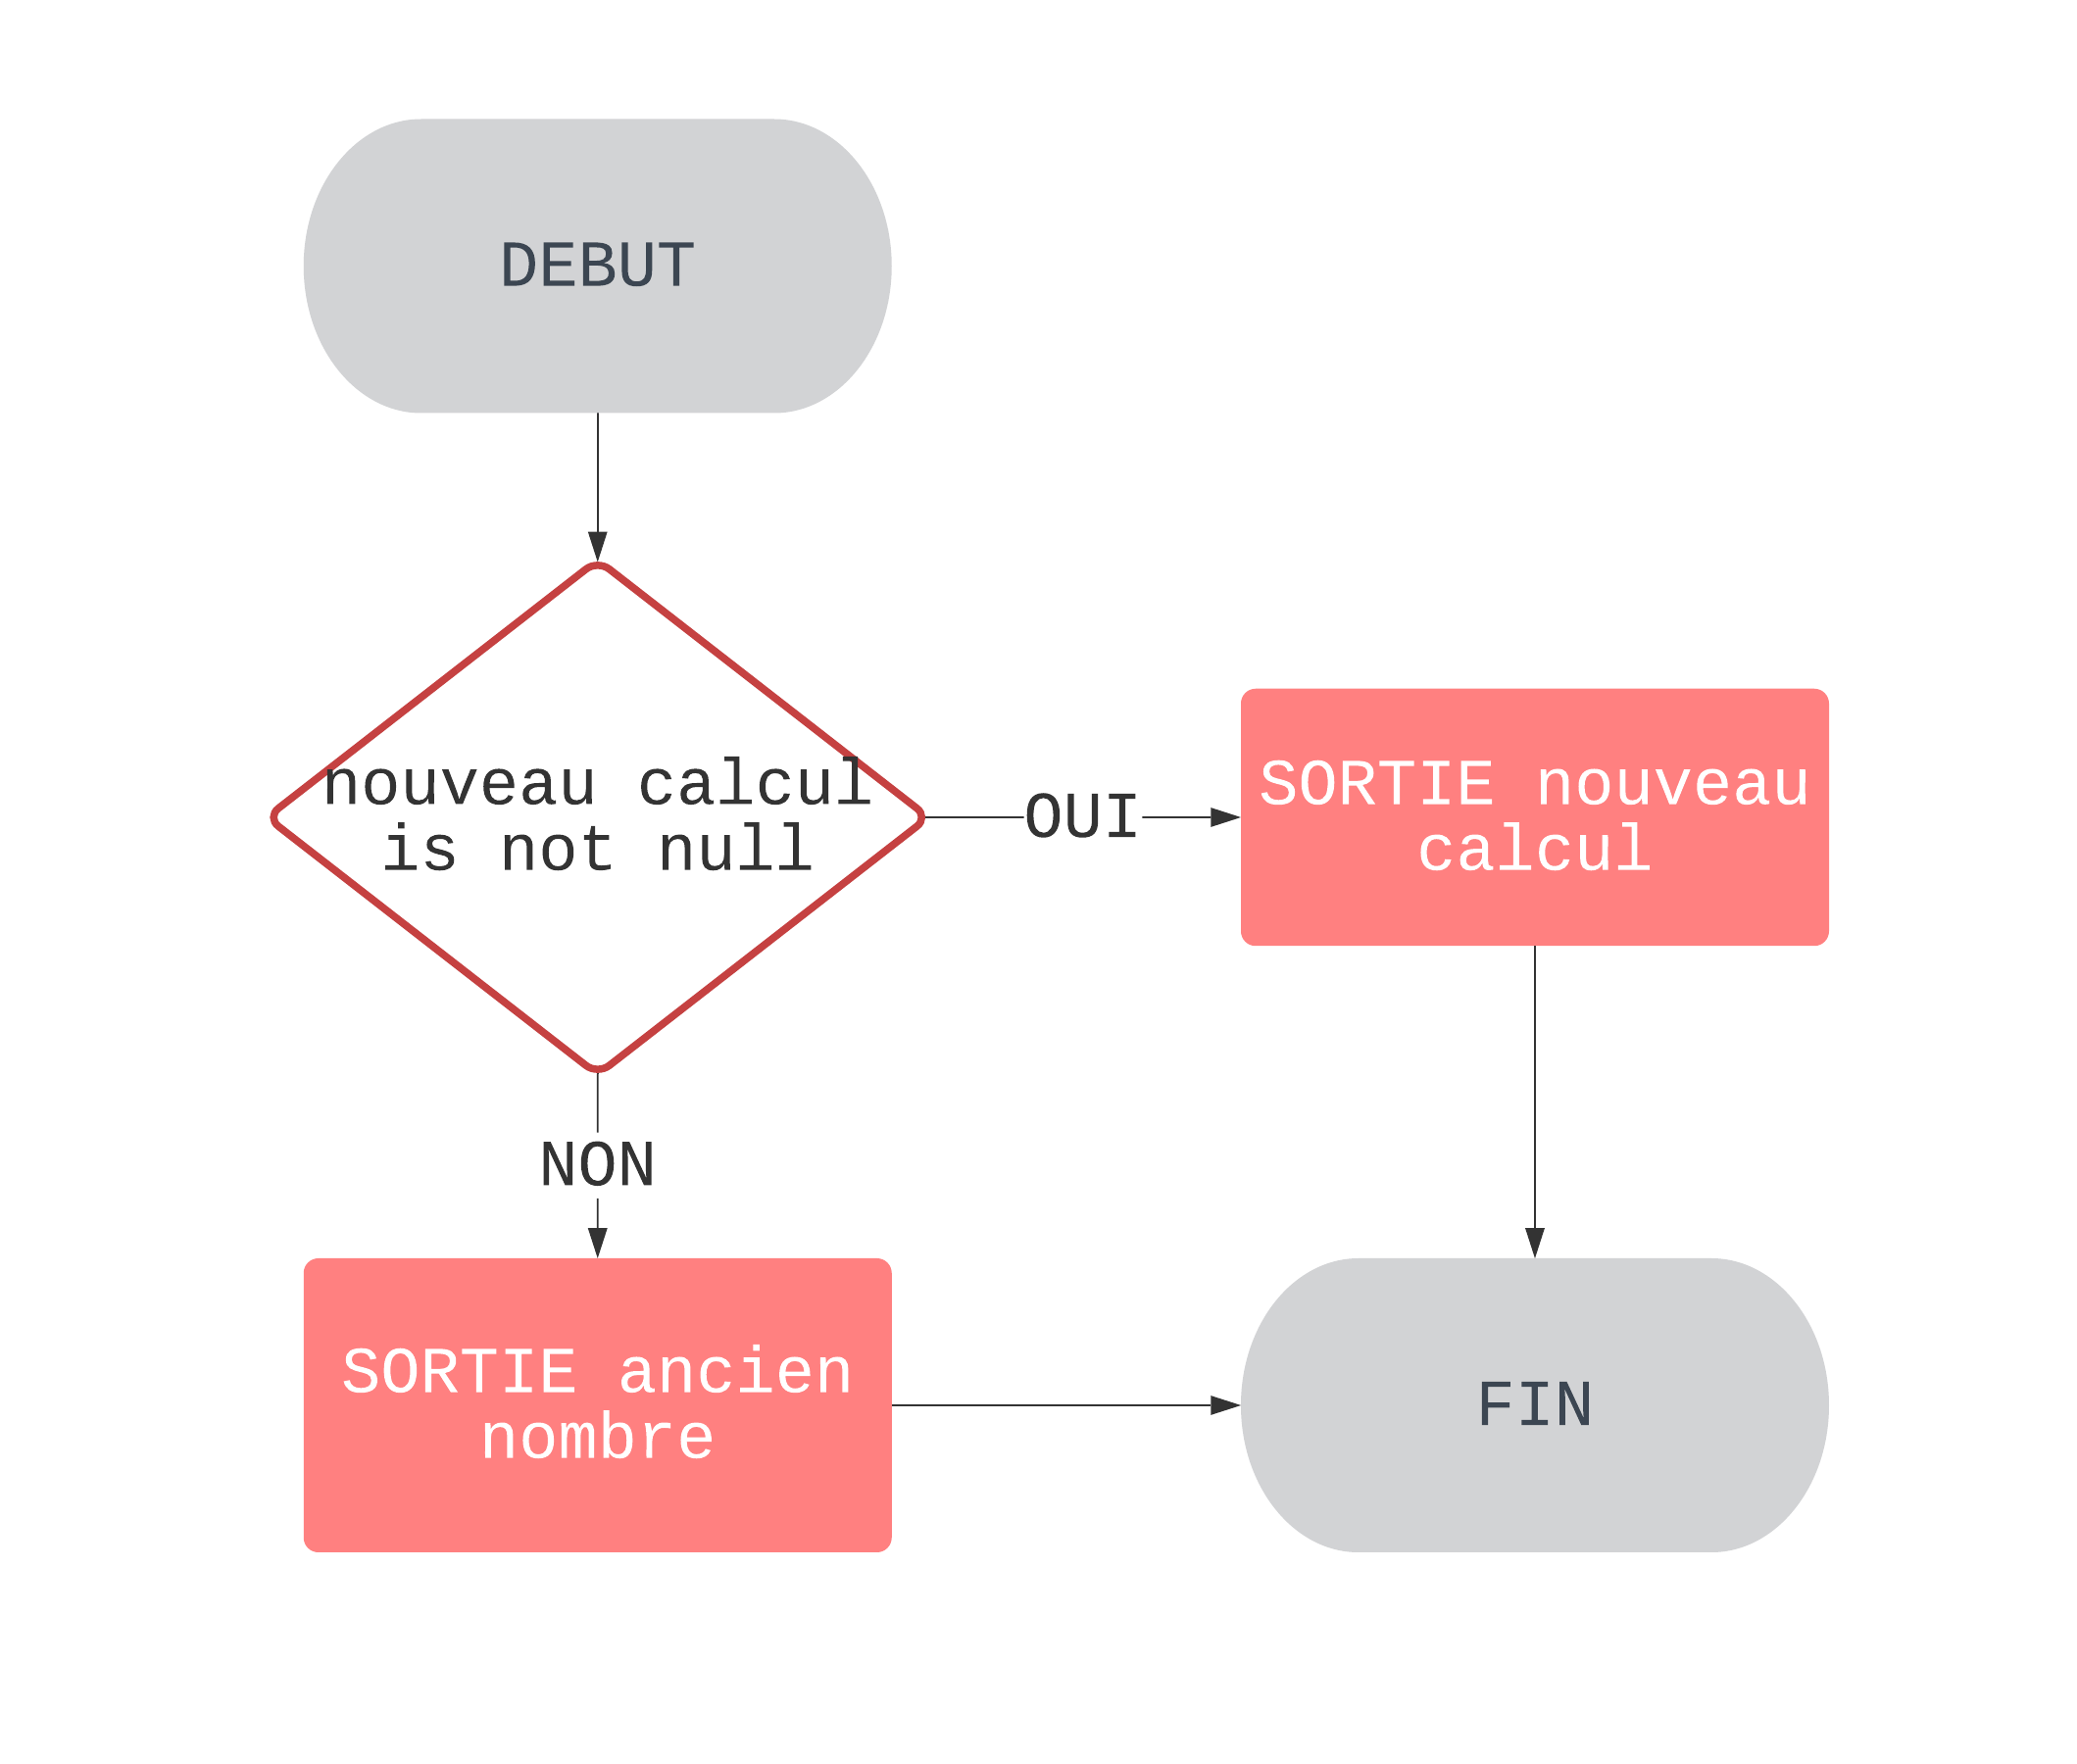
\includegraphics[scale=0.12]{Static/Algo_nombre_victimes.png} 
      \end{center}
        \caption{Algorigramme de fiabilisation du nombre de victime}  \label{fig:xray}
\end{figure}

Avec ces nouvelles valeurs, nous avons proc\'ed\'e au redressement de la nature du sinistre. Si le nombre de bless\'es ou de morts est sup\'erieur \`a z\'ero (0) alors on a un sinistre de nature 'Corporel'. Sinon si la charge est inf\'erieure ou \'egale \`a 100 000 dirham marocain et que le sinistre \'etait pr\'ec\'edemment qualifi\'e de 'Corporel' on le re-affecte en 'Materiel'. En effet, il n'y a aucune raison de le considérer comme un sinistre de nature 'Corporel'. Par contre, si aucune des conditions pr\'ec\'edentes n'est respect\'ee et on a la charge qui est strictement sup\'erieure \`a 100 000 dirham marocain ou un sinistre de nature 'Materiel' alors on conserve la valeur de la variable initiale '\textit{Nature\_Sinistre}'. Cet algorithme de redressement conduit \`a la cr\'eation d'une nouvelle variable '\textit{Nature\_Sinistre\_New}'.
\begin{figure}[H]
    \begin{center}
      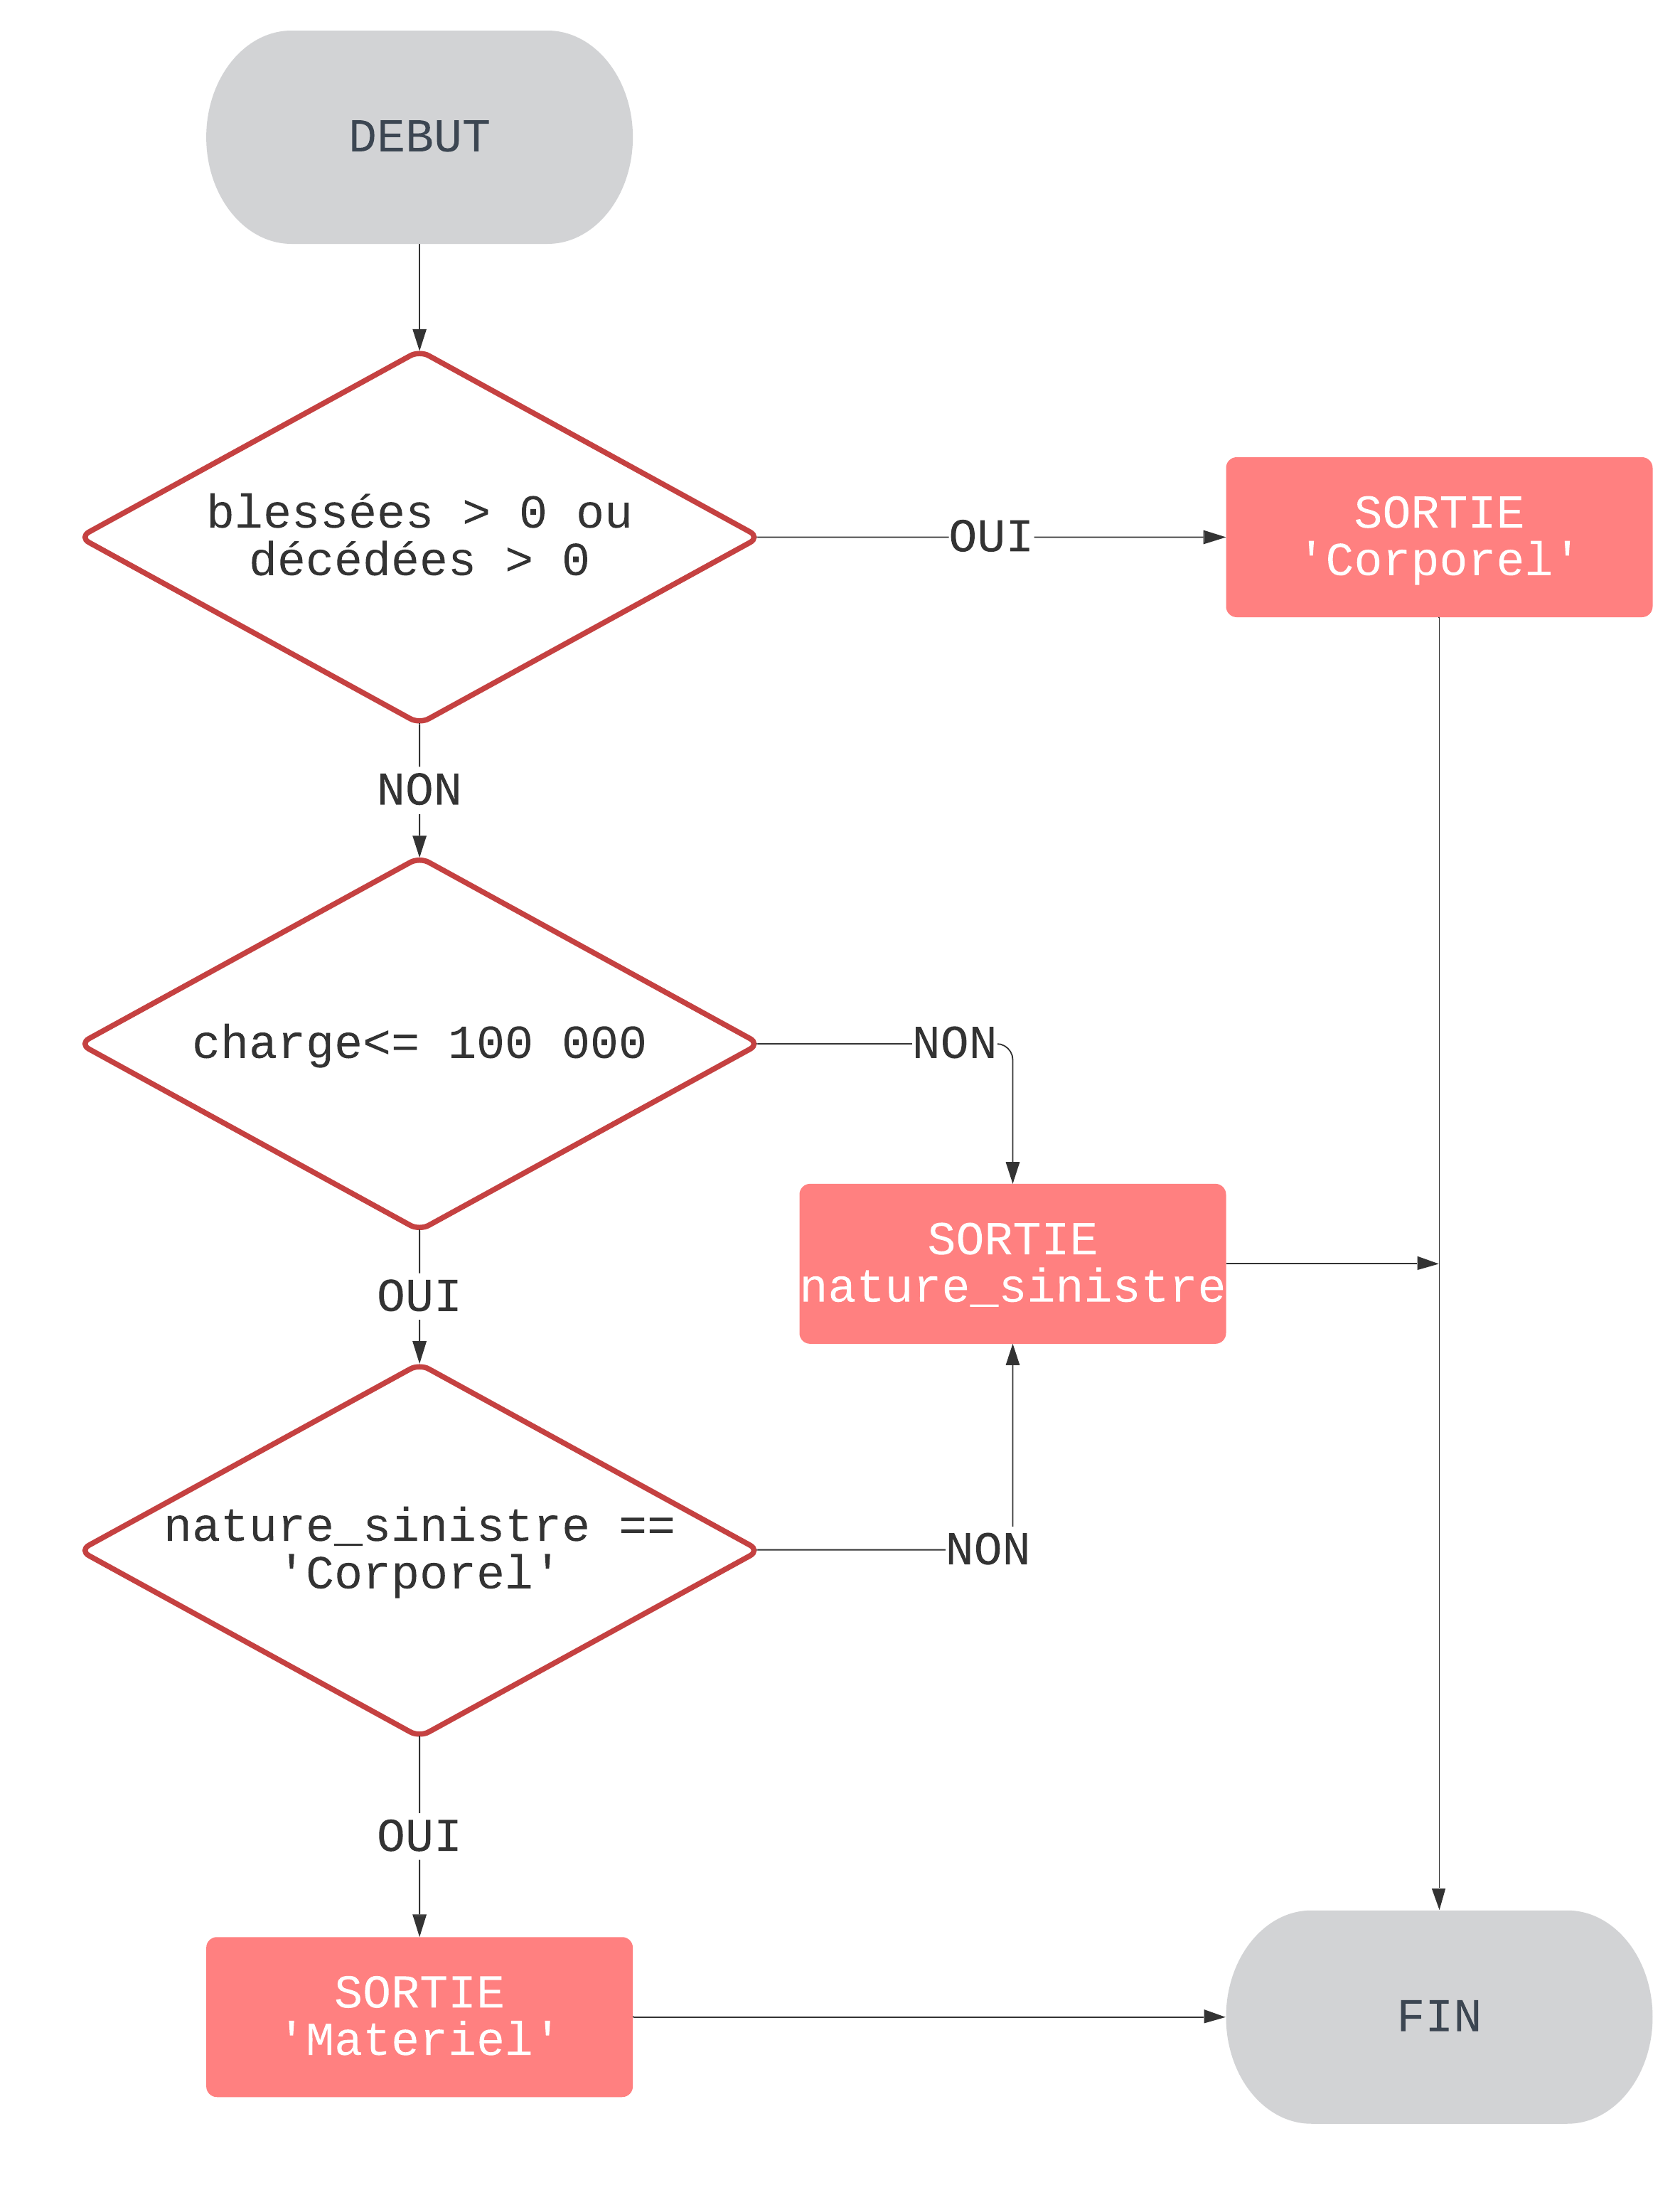
\includegraphics[scale=0.12]{Static/Algo_nature_sinistre.png} 
      \end{center}
        \caption{Algorigramme de fiabilisation de la nature du sinistre}  \label{fig:xray}
\end{figure}

\subsection{Algorithme de correction des probl\`emes d'encodages}
Les cibles de notre correction sont les mots du dictionnaire (pas les noms propres). L'algorithme utilis\'e se sert de la distance de Levenshtein pour identifier les corrections orthographiques les plus probables pour un mot : il s'agit des mots candidats. La distance de Levenshtein est une mesure de similarit\'e entre deux chaînes de caract\`eres. Elle est \'egale au nombre d'op\'erations \'el\'ementaires \`a r\'ealiser  pour transformer une chaîne M en une chaîne P. Il s'agit de :
\begin{itemize}[parsep=0cm,itemsep=0cm]
\item la substitution d'un caract\`ere;
\item l'insertion  ou l'ajout d'un caract\`ere;
\item la suppression ou l'effacement d'un caract\`ere.
\end{itemize}
Une fois la liste des mots candidats obtenue, l'algorithme compare ensuite tous les candidats à un dictionnaire de mots. La particularit\'e de ce dictionnaire est qu'il associe \`a chaque mot une fr\'equence d'apparition. La cl\'e est le mot et la valeur est la fr\'equence du mot. Le candidat ayant la plus forte fr\'equence d'apparition est plus susceptible d'être le résultat correct. En cas de co-occurrence un classement par ordre alphab\'etique est effectu\'e. Cet algorithme est impl\'ement\'e en Python par la biblioth\`eque SpellChecker. L'algorigramme mis en oeuvre pour corriger nos anomalies est le suivant : 
\begin{figure}[H]
    \begin{center}
      \includegraphics[scale=0.50]{Static/algo_spellchecker.png} 
      \end{center}
        \caption{Algorigramme de correction d'orthographe}  \label{fig:xray}
\end{figure}

\subsection{Fiabilisation des variables indicatrices}
Tout montant strictement sup\'erieur \`a z\'ero (0) doit \^etre mat\'erialis\'e par la modalit\'e 'Y' au niveau de la variable indicatrice. La correction de ces incoh\'erences est donc faite \`a l'aide de l'algorithme suivant: si le montant est sup\'erieur \`a  z\'ero (0), on affecte \`a une nouvelle variable indicatrice la valeur 'Y'. Dans le cas contraire, c'est la valeur 'N' qui est retournée afin de signifier qu'il n'y a pas de frais. La correction aboutit \`a la cr\'eation d'une nouvelle colonne afin de ne pas alt\'erer les donn\'ees existantes. L'algorithme mis en place \`a permis de corriger les incoh\'erences et d'imputer les valeurs manquantes des variables indicatrices.
%\newpage
\begin{figure}[H]
    \begin{center}
      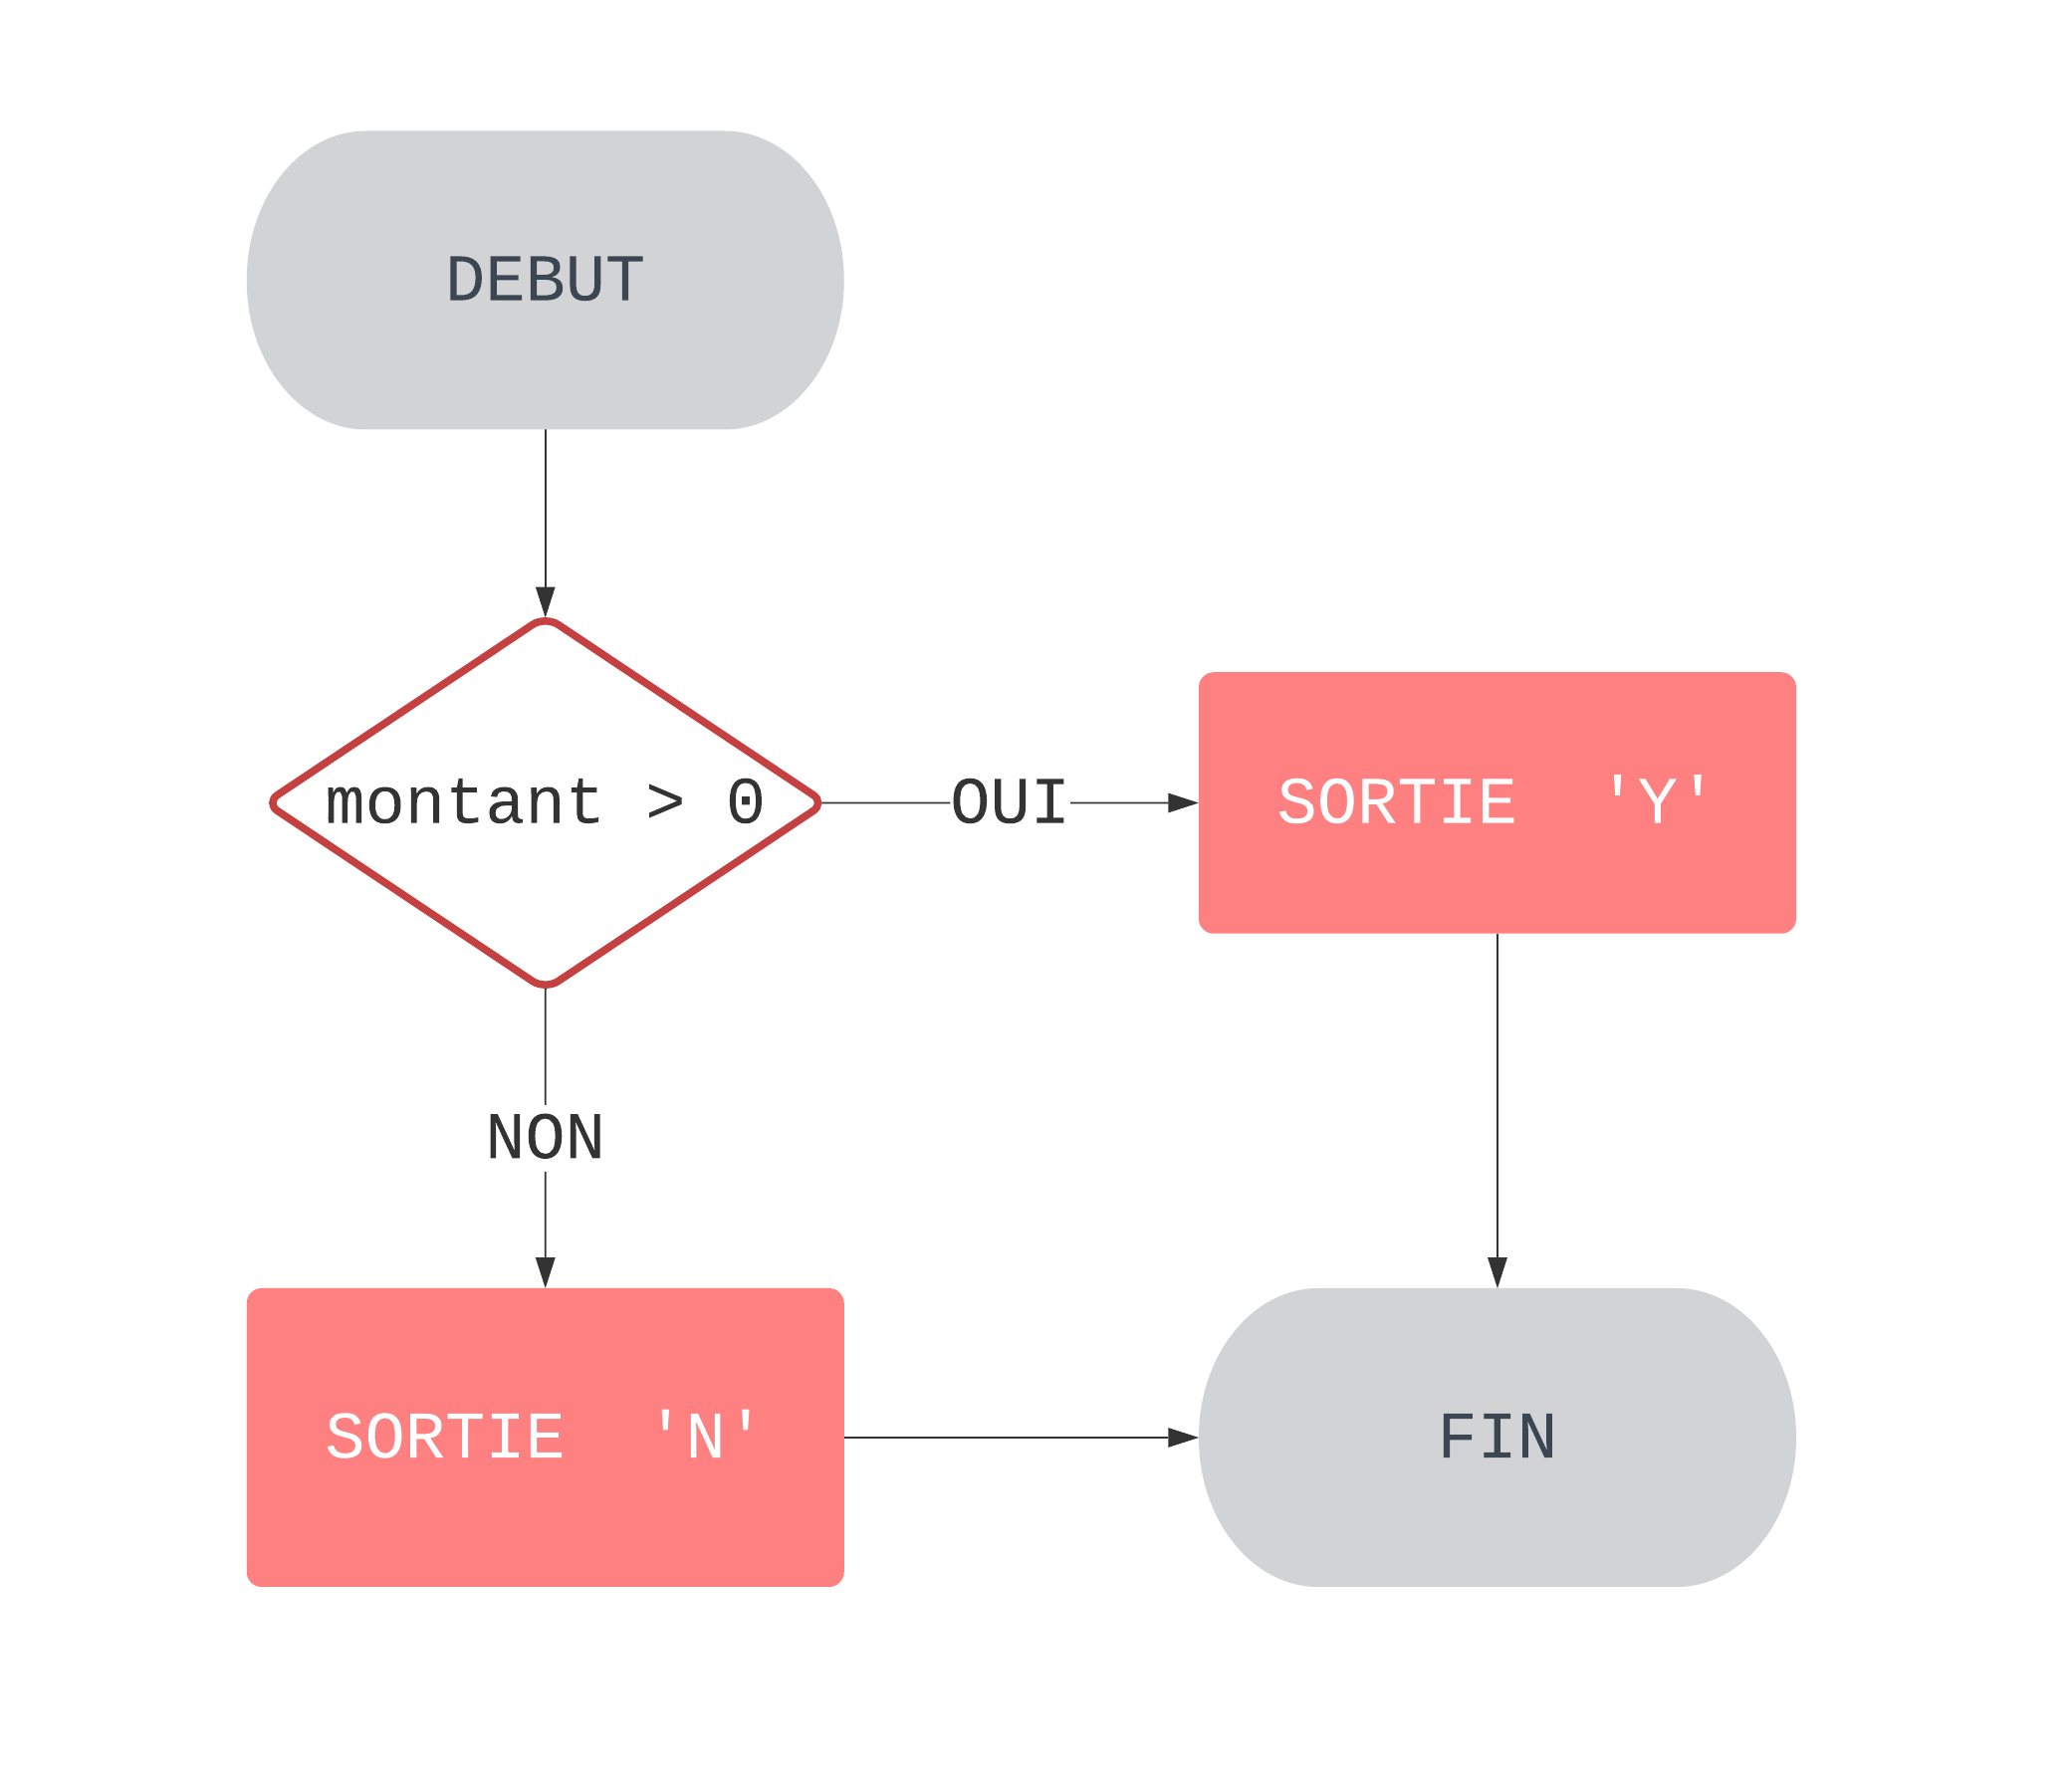
\includegraphics[scale=0.12]{Static/Algorithm_INDICATRICE.png} 
      \end{center}
        \caption{Algorigramme de r\'esolution des incoh\'erences variable indicatrice - montant}  \label{fig:xray}
\end{figure}

\section*{Conclusion}
Ce chapitre a fait l’objet d’un exposé des résultats obtenus suite à l'\'evaluation et \`a l'application des différents algorithmes de redressement proposés sur les donn\'ees du socle. Les anomalies ont \'et\'e d\'etect\'ees sur quatre (4) dimensions :  la compl\'etude, l'unicit\'e, la validit\'e et la coh\'erence. Mais toutes les anomalies ne sont pas nécessairement des erreurs. Les algorithmes de correction appliqu\'ees ont permis d'améliorer la qualit\'e des extractions reçues.


%Conclusion Generale
\cleardoublepage
\phantomsection
\addcontentsline{toc}{part}{CONCLUSION G\'EN\'ERALE}

\vspace*{0.5cm}
\section*{\centering \Huge Conclusion G\'en\'erale}
\titlerule[2.0pt]
\vspace{1cm}
Le problème crucial que pose la qualité des données \`a la \acrlong{df}, nous a amené \`a mettre en place Apache Griffin, un outil d'\'evaluation de la qualit\'e des donn\'ees, afin de pouvoir d\'etecter les anomalies dans les donn\'ees du socle, pour par la suite proposer des algorithmes de correction. Afin de mener \`a bien cette t\^ache, nous nous sommes attel\'es \`a comprendre au pr\'ealable le cadre d'analyse th\'eorique de la qualit\'e. Cette compr\'ehension \`a par ricochet favoriser la compr\'ehension de l'outil Apache Griffin, et permet une meilleure compr\'ehension de ses fonctionnalit\'es. \\

Face aux exigences en termes de qualit\'e et de service de la \acrshort{df}, nous avons mis en œuvre nos connaissances techniques afin de pouvoir adapter l'outil aux besoins formul\'es. Cette adaptation a permis une \'evaluation efficace de la qualit\'e des donn\'ees du socle et favoris\'e la mise en \'evidence de plusieurs irr\'egularit\'es suivant les dimensions suivantes: Compl\'etude, Unicit\'e, Validit\'e et Coh\'erence. La suite du projet consistait \`a apporter des correctifs aux anomalies d\'etect\'ees. Ce qui nous a amen\'e \`a \'ecrire en PySpark des algorithmes de fiabilisation des donn\'ees entachées d'irrégularités. La visualisation des m\'etriques sur le tableau de bord r\'ealis\'e \`a cet effet, permet aux d\'ecideurs de pouvoir suivre l'\'evolution de la qualit\'e des diff\'erentes donn\'ees au fil du temps.\\

La prochaine \'etape du volet qualit\'e dans la politique de gouvernance des donn\'ees du socle, doit inclure la d\'efinition claire et nette des m\'etriques et des seuils de m\^eme que l'int\'egration de l'outil dans leur architecture. La gestion de la qualit\'e doit donc commencer par un plan et une strat\'egie bien document\'ee. Ce qui va permettre de configurer les outils pour \'evaluer la qualit\'e. Les r\'esultats obtenus, permettront de mesurer l'ampleur des problèmes de qualité des données et de déterminer si l'acquisition des données et le processus d'analyse sont adéquats. Enfin, la dernière composante qu'est l'amélioration de la qualité, doit permettre l'\'epuration des donn\'ees, la compr\'ehension de la non qualit\'e et la prise de mesures pour améliorer le processus. Ce qui permettra d'ajuster le plan et ainsi de suite.
%Bibliographie
\addcontentsline{toc}{chapter}{BIBLIOGRAPHIE}
\bibliographystyle{IEEEtranN}
%{\footnotesize \bibliography{References}}
\bibliography{References}
%Annexe
%\chapter*{ANNEXE}
\renewcommand{\thesection}{\Alph{section}}
\setcounter{section}{0}

\begin{appendices}%\renewcommand{\thesection}{\Alph{section}}
\pagenumbering{alph}
\appendixheaderon

\section{Méthode de travail agile : SCRUM}
\label{ann:annexe1}
\subsection{Rôles}
\begin{enumerate}[parsep=0cm,itemsep=0cm]
\item \textbf{ Le \textit{«Product Owner»} ou \textit{«PO»} }: il porte la vision du produit à réaliser. Il travaille en collaboration directe avec l’équipe de développement et a notamment la charge de remplir le\textit{ «Product Backlog»} et de déterminer la priorité des \textit{«user stories»}\footnote{phrase simple, rédigée dans un langage courant, qui permet de décrire avec suffisamment de précision le contenu d’une fonctionnalité\\} à réaliser. 

\item \textbf{Le \textit{«Scrum Master»} ou \textit{«SM»}} : Il ne faut surtout pas le confondre avec un chef de projet. Il facilite le dialogue et le travail entre les différents intervenants, de façon à ce que l’équipe soit pleinement productive. 

\item \textbf{L’équipe de développement} : généralement composée de 4 à 6 personnes de plusieurs profils, elle est chargée de transformer les besoins exprimés par le \textit{«Product Owner»}  en fonctionnalités réelles, opérationnelles et utilisables. 
\end{enumerate}

\subsection{Réunions}
\begin{enumerate}[parsep=0cm,itemsep=0cm]
\item \textbf{Planification du \textit{Sprint}} (Sprint = itération) : au cours de cette réunion, l'équipe de développement sélectionne les éléments prioritaires du \textit{«Product Backlog»}\footnote{liste ordonnancée des exigences fonctionnelles et non fonctionnelles du projet} qu'elle pense pouvoir réaliser au cours du \textit{Sprint}.

\item \textbf{Revue de Sprint} : au cours de cette réunion qui a lieu à la fin du \textit{Sprint}, l'équipe de développement présente les fonctionnalités terminées au cours du \textit{Sprint} et recueille les feedbacks du \textit{«Product Owner»} et des utilisateurs finaux. C'est également le moment d'anticiper le périmètre des prochains \textit{Sprints} et d'ajuster au besoin la planification de \textit{release} (nombre de \textit{Sprints} restants).

\item \textbf{Rétrospective de \textit{Sprint}} : la rétrospective qui a généralement lieu après la revue de \textit{Sprint} est l'occasion de s'améliorer (productivité, qualité, efficacité, conditions de travail, etc) à la lueur du "vécu" sur le \textit{Sprint} écoulé (principe d'amélioration continue).

\item \textbf{Mêlée quotidienne}  : il s'agit d'une réunion de synchronisation de l'équipe de développement qui se fait debout en 15 minutes maximum au cours de laquelle chacun répond principalement à 3 questions : \textit{«Qu'est ce que j'ai terminé depuis la dernière mêlée ? Qu'est ce que j'aurai terminé d'ici la prochaine mêlée ? Quels obstacles me retardent ?»}.
\end{enumerate}

\subsection{Artefacts}
\begin{enumerate}[parsep=0cm,itemsep=0cm]
\item \textbf{Le \textit{Sprint}}: il s'agit d'une période pendant laquelle un travail spécifique doit être mené à bien avant de faire l'objet d'une révision.
\item \textbf{Le \textit{Product Backlog}}: il s'agit d'une liste hiérarchisée des exigences initiales du client concernant le produit à réaliser.
\item \textbf{Le \textit{Sprint Backlog}}: c'est le plan détaillé de la réalisation de l'objectif du \textit{Sprint}, défini lors de la réunion de planification du \textit{Sprint}.
\item \textbf{Le \textit{Task Board}} : outil central du \textit{Sprint} scrum, ce tableau de bord du projet permet de suivre en temps réel la progression de la réalisation des différentes tâches. Il pr\'esente les tâches à faire, les tâches en cours et les tâches terminées.
\item \textbf{Le \textit{Burndown Chart}} : il s’agit d’un graphique simple permettant de visualiser le degré d’avancement de chacune des tâches.
\end{enumerate}

\end{appendices}

\section{Compl\'ement sur les distances}
On retiendra essentiellement \cite{bensalem}:
\begin{itemize}[parsep=0cm,itemsep=0cm]
\item pour les mesures impliquant des chaînes de caractères on a les mesures lexicographiques (distances Levenshtein, distance Q-gram, distance de Jaro-Winkler) et les mesures phon\'etiques (Soundex, Double Metaphore, New York State Identification and Intelligence System, une combinaison des mesures phon\'etique et lexicographique);
\item pour les donn\'ees num\'eriques une transformation en chaînes de caractères peut \^etre appliqu\'ee;
\item pour les dates on peut effectuer un calcul de différence entre les jours, les mois et les années
\end{itemize} 


\cleardoublepage
\phantomsection
\addcontentsline{toc}{chapter}{Table des matières}
\tableofcontents

\end{document}